% Options for packages loaded elsewhere
\PassOptionsToPackage{unicode}{hyperref}
\PassOptionsToPackage{hyphens}{url}
\documentclass[
  english,
]{article}
\usepackage{xcolor}
\usepackage[margin=0.5in]{geometry}
\usepackage{amsmath,amssymb}
\setcounter{secnumdepth}{5}
\usepackage{iftex}
\ifPDFTeX
  \usepackage[T1]{fontenc}
  \usepackage[utf8]{inputenc}
  \usepackage{textcomp} % provide euro and other symbols
\else % if luatex or xetex
  \usepackage{unicode-math} % this also loads fontspec
  \defaultfontfeatures{Scale=MatchLowercase}
  \defaultfontfeatures[\rmfamily]{Ligatures=TeX,Scale=1}
\fi
% \usepackage{lmodern}
\ifPDFTeX\else
  % xetex/luatex font selection
\fi
% Use upquote if available, for straight quotes in verbatim environments
\IfFileExists{upquote.sty}{\usepackage{upquote}}{}
\IfFileExists{microtype.sty}{% use microtype if available
  \usepackage[]{microtype}
  \UseMicrotypeSet[protrusion]{basicmath} % disable protrusion for tt fonts
}{}
\makeatletter
\@ifundefined{KOMAClassName}{% if non-KOMA class
  \IfFileExists{parskip.sty}{%
    \usepackage{parskip}
  }{% else
    \setlength{\parindent}{0pt}
    \setlength{\parskip}{6pt plus 2pt minus 1pt}}
}{% if KOMA class
  \KOMAoptions{parskip=half}}
\makeatother
\usepackage{color}
\usepackage{fancyvrb}
\newcommand{\VerbBar}{|}
\newcommand{\VERB}{\Verb[commandchars=\\\{\}]}
\DefineVerbatimEnvironment{Highlighting}{Verbatim}{commandchars=\\\{\}}
% Add ',fontsize=\small' for more characters per line
\newenvironment{Shaded}{}{}
\newcommand{\AlertTok}[1]{\textcolor[rgb]{1.00,0.00,0.00}{\textbf{#1}}}
\newcommand{\AnnotationTok}[1]{\textcolor[rgb]{0.38,0.63,0.69}{\textbf{\textit{#1}}}}
\newcommand{\AttributeTok}[1]{\textcolor[rgb]{0.49,0.56,0.16}{#1}}
\newcommand{\BaseNTok}[1]{\textcolor[rgb]{0.25,0.63,0.44}{#1}}
\newcommand{\BuiltInTok}[1]{\textcolor[rgb]{0.00,0.50,0.00}{#1}}
\newcommand{\CharTok}[1]{\textcolor[rgb]{0.25,0.44,0.63}{#1}}
\newcommand{\CommentTok}[1]{\textcolor[rgb]{0.38,0.63,0.69}{\textit{#1}}}
\newcommand{\CommentVarTok}[1]{\textcolor[rgb]{0.38,0.63,0.69}{\textbf{\textit{#1}}}}
\newcommand{\ConstantTok}[1]{\textcolor[rgb]{0.53,0.00,0.00}{#1}}
\newcommand{\ControlFlowTok}[1]{\textcolor[rgb]{0.00,0.44,0.13}{\textbf{#1}}}
\newcommand{\DataTypeTok}[1]{\textcolor[rgb]{0.56,0.13,0.00}{#1}}
\newcommand{\DecValTok}[1]{\textcolor[rgb]{0.25,0.63,0.44}{#1}}
\newcommand{\DocumentationTok}[1]{\textcolor[rgb]{0.73,0.13,0.13}{\textit{#1}}}
\newcommand{\ErrorTok}[1]{\textcolor[rgb]{1.00,0.00,0.00}{\textbf{#1}}}
\newcommand{\ExtensionTok}[1]{#1}
\newcommand{\FloatTok}[1]{\textcolor[rgb]{0.25,0.63,0.44}{#1}}
\newcommand{\FunctionTok}[1]{\textcolor[rgb]{0.02,0.16,0.49}{#1}}
\newcommand{\ImportTok}[1]{\textcolor[rgb]{0.00,0.50,0.00}{\textbf{#1}}}
\newcommand{\InformationTok}[1]{\textcolor[rgb]{0.38,0.63,0.69}{\textbf{\textit{#1}}}}
\newcommand{\KeywordTok}[1]{\textcolor[rgb]{0.00,0.44,0.13}{\textbf{#1}}}
\newcommand{\NormalTok}[1]{#1}
\newcommand{\OperatorTok}[1]{\textcolor[rgb]{0.40,0.40,0.40}{#1}}
\newcommand{\OtherTok}[1]{\textcolor[rgb]{0.00,0.44,0.13}{#1}}
\newcommand{\PreprocessorTok}[1]{\textcolor[rgb]{0.74,0.48,0.00}{#1}}
\newcommand{\RegionMarkerTok}[1]{#1}
\newcommand{\SpecialCharTok}[1]{\textcolor[rgb]{0.25,0.44,0.63}{#1}}
\newcommand{\SpecialStringTok}[1]{\textcolor[rgb]{0.73,0.40,0.53}{#1}}
\newcommand{\StringTok}[1]{\textcolor[rgb]{0.25,0.44,0.63}{#1}}
\newcommand{\VariableTok}[1]{\textcolor[rgb]{0.10,0.09,0.49}{#1}}
\newcommand{\VerbatimStringTok}[1]{\textcolor[rgb]{0.25,0.44,0.63}{#1}}
\newcommand{\WarningTok}[1]{\textcolor[rgb]{0.38,0.63,0.69}{\textbf{\textit{#1}}}}
\usepackage{longtable,booktabs,array}
\newcounter{none} % for unnumbered tables
\usepackage{calc} % for calculating minipage widths
% Correct order of tables after \paragraph or \subparagraph
\usepackage{etoolbox}
\makeatletter
\patchcmd\longtable{\par}{\if@noskipsec\mbox{}\fi\par}{}{}
\makeatother
% Allow footnotes in longtable head/foot
\IfFileExists{footnotehyper.sty}{\usepackage{footnotehyper}}{\usepackage{footnote}}
\makesavenoteenv{longtable}
\usepackage{graphicx}
\makeatletter
\newsavebox\pandoc@box
\newcommand*\pandocbounded[1]{% scales image to fit in text height/width
  \sbox\pandoc@box{#1}%
  \Gscale@div\@tempa{\textheight}{\dimexpr\ht\pandoc@box+\dp\pandoc@box\relax}%
  \Gscale@div\@tempb{\linewidth}{\wd\pandoc@box}%
  \ifdim\@tempb\p@<\@tempa\p@\let\@tempa\@tempb\fi% select the smaller of both
  \ifdim\@tempa\p@<\p@\scalebox{\@tempa}{\usebox\pandoc@box}%
  \else\usebox{\pandoc@box}%
  \fi%
}
% Set default figure placement to htbp
\def\fps@figure{htbp}
\makeatother
\ifLuaTeX
\usepackage[bidi=basic,shorthands=off]{babel}
\else
\usepackage[bidi=default,shorthands=off]{babel}
\fi
\ifLuaTeX
  \usepackage{selnolig} % disable illegal ligatures
\fi
\setlength{\emergencystretch}{3em} % prevent overfull lines
\providecommand{\tightlist}{%
  \setlength{\itemsep}{0pt}\setlength{\parskip}{0pt}}
\usepackage[]{natbib}
\bibliographystyle{plainnat}
\makeatletter
\@ifpackageloaded{subcaption}{}{\usepackage{subcaption}}
\@ifpackageloaded{caption}{}{\usepackage{caption}}
\captionsetup[subfigure]{margin=0.5em}
\AtBeginDocument{%
\renewcommand*\figurename{Figure}
\renewcommand*\tablename{Table}
}
\AtBeginDocument{%
\renewcommand*\listfigurename{List of Figures}
\renewcommand*\listtablename{List of Tables}
}
\newcounter{pandoccrossref@subfigures@footnote@counter}
\newenvironment{pandoccrossrefsubfigures}{%
\setcounter{pandoccrossref@subfigures@footnote@counter}{0}
\begin{figure}\centering%
\gdef\global@pandoccrossref@subfigures@footnotes{}%
\DeclareRobustCommand{\footnote}[1]{\footnotemark%
\stepcounter{pandoccrossref@subfigures@footnote@counter}%
\ifx\global@pandoccrossref@subfigures@footnotes\empty%
\gdef\global@pandoccrossref@subfigures@footnotes{{##1}}%
\else%
\g@addto@macro\global@pandoccrossref@subfigures@footnotes{, {##1}}%
\fi}}%
{\end{figure}%
\addtocounter{footnote}{-\value{pandoccrossref@subfigures@footnote@counter}}
\@for\f:=\global@pandoccrossref@subfigures@footnotes\do{\stepcounter{footnote}\footnotetext{\f}}%
\gdef\global@pandoccrossref@subfigures@footnotes{}}
\@ifpackageloaded{float}{}{\usepackage{float}}
\floatstyle{ruled}
\@ifundefined{c@chapter}{\newfloat{codelisting}{h}{lop}}{\newfloat{codelisting}{h}{lop}[chapter]}
\floatname{codelisting}{Listing}
\newcommand*\listoflistings{\listof{codelisting}{List of Listings}}
\makeatother
\usepackage{bookmark}
\IfFileExists{xurl.sty}{\usepackage{xurl}}{} % add URL line breaks if available
\urlstyle{same}
% fallback for those not using the hyperref driver hyperxmp:
\makeatletter
\@ifundefined{xmpquote}{\newcommand{\xmpquote}[1]{#1}}{}
\makeatother
\hypersetup{
  pdftitle={Active Inference Multi-Track Exemplar},
  pdfauthor={Daniel Ari Friedman},
  pdflang={en},
  colorlinks=true,linkcolor=red,urlcolor=red,citecolor=red,anchorcolor=red,filecolor=red,
  pdfcreator={LaTeX via pandoc}}

\title{Active Inference Multi-Track Exemplar}
\author{Daniel Ari Friedman}
\date{}

\IfFileExists{seqsplit.sty}{\usepackage{seqsplit}}{\newcommand{\seqsplit}[1]{#1}}
\protected\def\breakseq#1{\seqsplit{#1}}
\protected\def\breaktt#1{\begingroup\ttfamily\seqsplit{#1}\endgroup}
\title{Active Inference Multi-Track Exemplar}
\author{Daniel Ari Friedman\\\footnotesize{Active Inference Institute}\\\footnotesize{\texttt{daniel@activeinference.institute}}\\\footnotesize{\href{https://orcid.org/0000-0001-6232-9096}{ORCID: 0000-0001-6232-9096}} \\ \footnotesize{DOI: \href{https://doi.org/10.5281/zenodo.20417021}{10.5281/zenodo.20417021}}}
\date{2026-06-26}

\usepackage{amsmath,amssymb}
\usepackage{graphicx}
% Dense 9pt body via class-agnostic global rescaling (works on the default
% `article` class). Signature: \changefontsize[<baselineskip>]{<size>} — the
% baselineskip is the OPTIONAL bracketed arg; a second brace would print as text.
\usepackage{fontsize}
\changefontsize[11pt]{9pt}

\begin{document}
\maketitle

\thispagestyle{empty}
\setlength{\parskip}{0pt}
\setlength{\itemsep}{0pt}
\begin{samepage}
\scriptsize

\section*{BEGINNING OF TRANSMISSION}\label{beginning-of-transmission}

\textbf{State:} published

\textbf{Pairing:} complete (DOI, GitHub, SHA-256, Zenodo URL)

\subsubsection*{Release metadata}

{\def\LTcaptype{none} % do not increment counter
\begin{longtable}[]{@{}
  >{\raggedright\arraybackslash}p{(\linewidth - 2\tabcolsep) * \real{0.5000}}
  >{\raggedright\arraybackslash}p{(\linewidth - 2\tabcolsep) * \real{0.5000}}@{}}
\toprule\noalign{}
\begin{minipage}[b]{\linewidth}\raggedright
Field
\end{minipage} & \begin{minipage}[b]{\linewidth}\raggedright
Value
\end{minipage} \\
\midrule\noalign{}
\endhead
\bottomrule\noalign{}
\endlastfoot
Title & Active Inference Multi-Track Exemplar \\
Version & 0.3.2 \\
Concept DOI & 10.5281/zenodo.20417021 \\
Version DOI & 10.5281/zenodo.20931870 \\
GitHub &
\url{https://github.com/docxology/template_active_inference/releases/tag/v0.3.2} \\
Zenodo & \url{https://zenodo.org/records/20417021} \\
SHA-256 & \breaktt{f191b48f94394cab…} \\
SHA-512 & pending \\
\end{longtable}
}

\subsubsection*{How to verify}

\begin{itemize}
\tightlist
\item
  Scan \textbf{Integrity} QR and compare the embedded SHA-256 prefix to
  the table above.
\item
  Scan \textbf{Zenodo} / \textbf{GitHub} QR codes and confirm they
  resolve to this release pairing.
\item
  Full hashes and structured fields:
  \breaktt{../data/transmission\_manifest.json}.
\end{itemize}

\begin{figure}
\centering
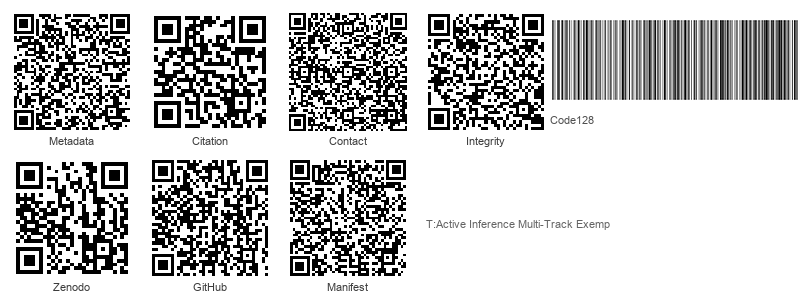
\includegraphics[width=0.98\linewidth,height=0.5\textheight,keepaspectratio,alt={Integrity QR strip}]{../figures/transmission_integrity_strip.png}
\caption{Integrity QR strip}
\end{figure}

Structured manifest: \breaktt{../data/transmission\_manifest.json}

\begin{figure}
\centering
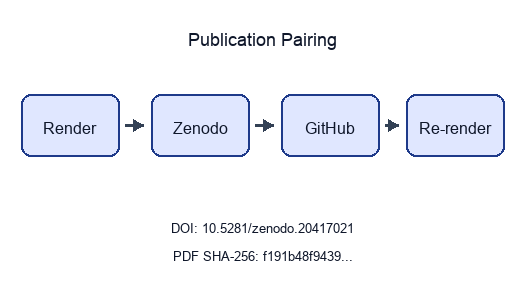
\includegraphics[width=0.35\linewidth,height=0.5\textheight,keepaspectratio,alt={Publication pairing flow}]{../figures/transmission_pairing.png}
\caption{Publication pairing flow}
\end{figure}

\textbf{Stego:} off |{} overlays text |{} barcodes on
|{} XMP on |{} manifest on \texorpdfstring{\ensuremath{\to}}{->} \texttt{./secure\_run.sh}

\end{samepage}
\newpage
\tableofcontents
\newpage


\newpage

\section{Sheaf Track Coverage}\label{sec:sheaf_coverage}

This page summarizes which \textbf{sheaf fragment tracks} are bound for
each IMRAD row in \breaktt{manuscript/sheaf/manifest.yaml}. The matrix is
regenerated at compose time.

\textbf{Totals:} 95 present / 95 bound / 0 missing (gray).

{\def\LTcaptype{none} % do not increment counter
\begin{longtable}[]{@{}ll@{}}
\toprule\noalign{}
Color & Meaning \\
\midrule\noalign{}
\endhead
\bottomrule\noalign{}
\endlastfoot
Black & Track \textbf{present} (bound and fragment exists) \\
White & \textbf{Absent} (not bound for this row) \\
Gray & \textbf{Missing} (bound but fragment file absent) \\
\end{longtable}
}

\subsection{Introduction}\label{introduction}

\begin{itemize}
\item
  \textbf{Introduction} \emph{(group)}
\item
  \textbf{Motivation and scope}
\item
  \textbf{Contributions} \#\# Methods
\item
  \textbf{Methods} \emph{(group)}
\item
  \textbf{Bernoulli--Ising analytical model}
\item
  \textbf{pymdp simulation harness}
\item
  \textbf{Lean formalization boundary}
\item
  \textbf{Sheaf composition} \#\# Results
\item
  \textbf{Results} \emph{(group)}
\item
  \textbf{Mutual-information parameter sweep}
\item
  \textbf{Free-energy decomposition}
\item
  \textbf{T-maze active-inference rollout}
\item
  \textbf{Validation invariants} \#\# Discussion
\item
  \textbf{Discussion} \emph{(group)}
\item
  \textbf{Limitations and outlook} \#\# Appendix
\item
  \textbf{Appendix} \emph{(group)}
\item
  \textbf{Appendix: full track coverage}
\end{itemize}

\begin{figure}
\centering
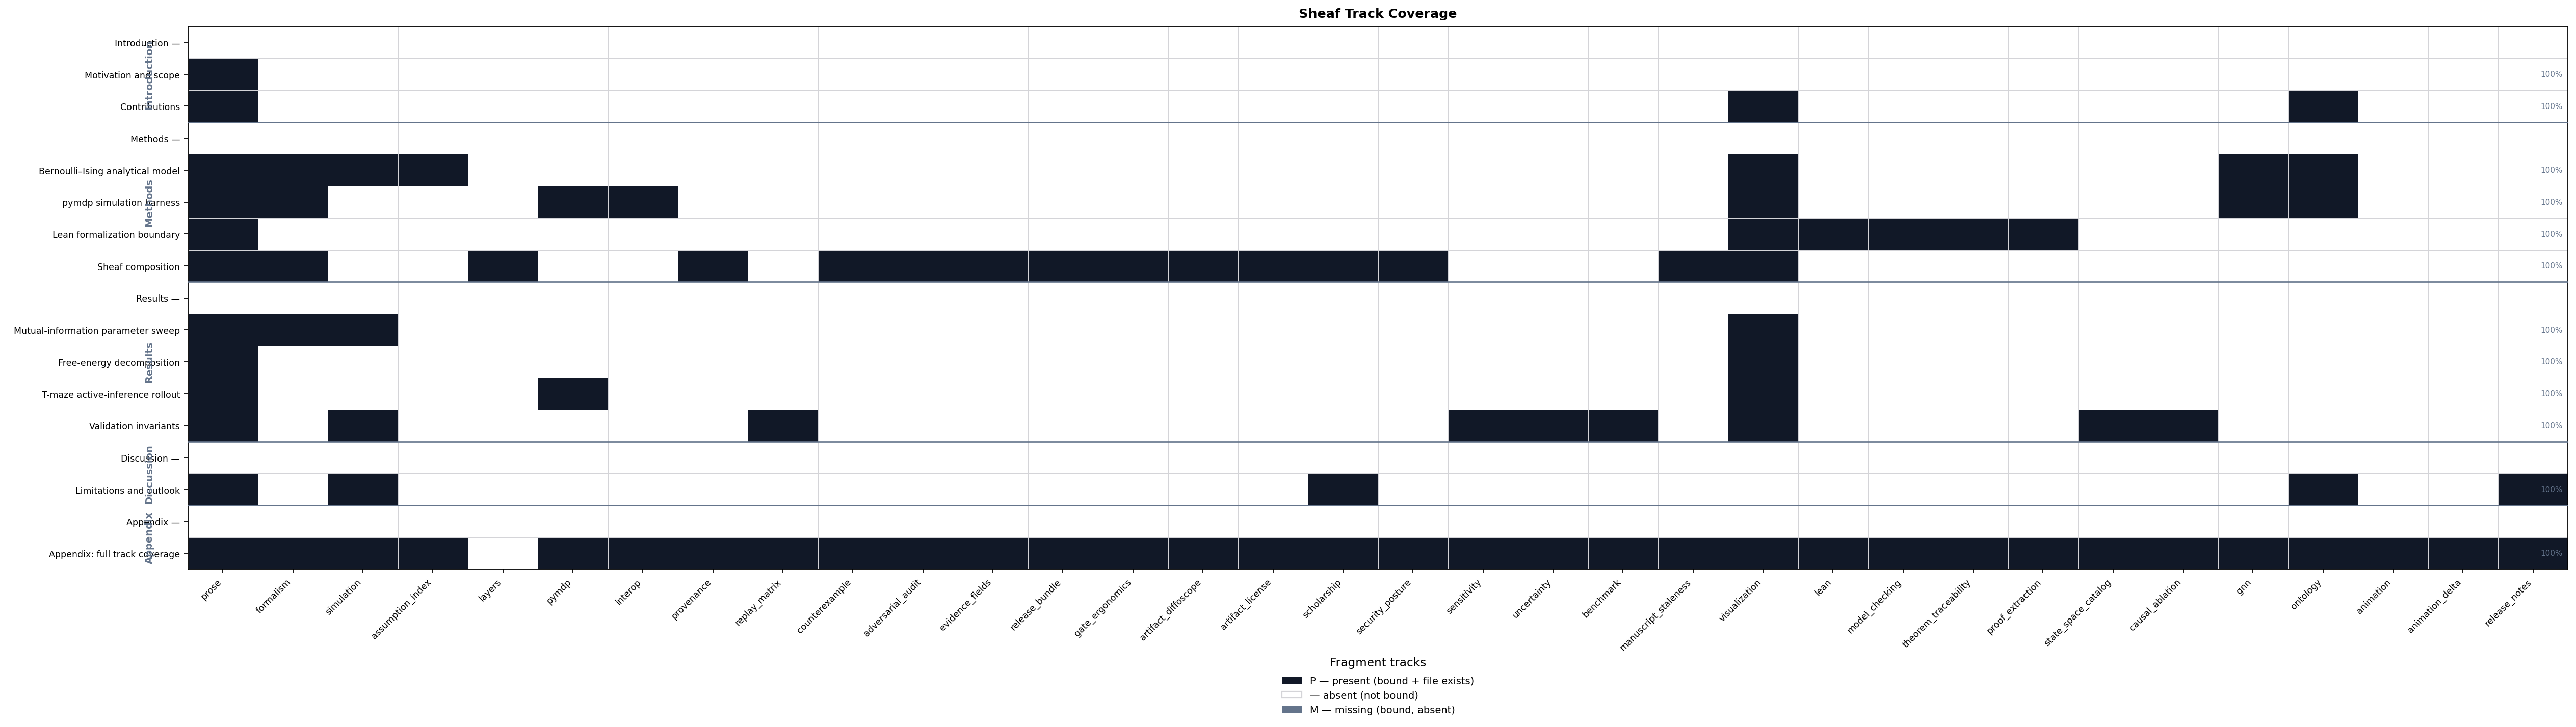
\includegraphics[width=0.95\linewidth,height=0.5\textheight,keepaspectratio,alt={Sheaf track coverage matrix: 17 IMRAD rows \texorpdfstring{\ensuremath{\times}}{x} 34 fragment columns. Black = present (P), white = absent (---), gray = missing (M). Counts: 95 present / 95 bound / 0 missing. Generated from output/data/sheaf\_coverage\_matrix.json.}]{../figures/sheaf_coverage_heatmap.png}
\caption{Sheaf track coverage matrix: 17 IMRAD rows \texorpdfstring{\ensuremath{\times}}{x} 34 fragment
columns. Black = present (P), white = absent (---), gray = missing (M).
Counts: 95 present / 95 bound / 0 missing. Generated from
\protect\breaktt{output/data/sheaf\_coverage\_matrix.json}.}\label{fig:sheaf_coverage_heatmap}
\end{figure}

Appendix row \breaktt{16\_appendix\_full\_sheaf.md} binds 33 fragment
track types as a composability proof (registry defines 34 types;
optional \texttt{layers} is methods-only).

\newpage

\section{Abstract}\label{sec:abstract}

We study a minimal Active Inference stack on toy models: a
Bernoulli--Ising analytical oracle, a pymdp T-maze rollout, and a
sheaf-indexed compose contract that binds 34 fragment tracks into 12
flat IMRAD sections. The methodological contribution is a discipline
rather than a domain finding: every reported number is hydrated from a
generated artifact and every cross-track claim is machine-checked before
rendering, so no figure or statistic can drift from the artifact that
produced it --- 6 sheaf axioms are verified before composition and 25
negative controls keep each failure path live. Claims are limited to
those models and their generated artifacts.

sec.~\ref{sec:sheaf_coverage} reports a 17-row coverage matrix (5 IMRAD
group headers) regenerated from the live manifest at compose time.
sec.~\ref{sec:methods_pymdp} documents the T-maze harness aligned with
\href{https://github.com/infer-actively/pymdp/tree/main/examples/experimental/sophisticated_inference}{pymdp
sophisticated\_inference examples}.

sec.~\ref{sec:results_invariants} records 12 / 12 invariant checks
passed. SI planning horizon: 2 steps. Sweep RMSE 0 nats bounds
analytical--empirical agreement on the coupling grid.

\newpage

\phantomsection
\addcontentsline{toc}{section}{Introduction}
\section*{Introduction}

\section{Motivation and scope}\label{sec:intro_motivation}

\subsection{Scientific scope}\label{scientific-scope}

This manuscript couples three tracks on toy Active Inference models: a
Bernoulli--Ising analytical oracle, a pymdp T-maze rollout, and a
sheaf-indexed assembly contract that binds 34 optional fragment tracks
under an IMRAD outline. The conceptual lineage is the free-energy and
active-inference literature
\citep{friston2010fep, buckley2017mathreview, parr2022active}, with
critical scope pressure from accounts that separate FEP's broad
organizing role from direct empirical brain claims
\citep{gershman2019fepbrain}. Here that distinction is operational: the
scientific claims stay within these models and their generated
artifacts, not biological agents.

\subsection{Manuscript structure}\label{manuscript-structure}

Three \textbf{scientific tracks} (analytical, pymdp, sheaf composition)
map onto 34 \textbf{composable fragment types} and 31 pipeline gates
(fig.~\ref{fig:multi_track_architecture}). sec.~\ref{sec:sheaf_coverage}
summarizes which fragment tracks bind to each manifest row.
sec.~\ref{sec:methods_sheaf} documents the compose pipeline, coverage
semantics (eq.~\ref{eq:coverage_cell}), and strict validation gates.

The pymdp track follows the
\href{https://github.com/infer-actively/pymdp/tree/main/examples/experimental/sophisticated_inference}{pymdp
sophisticated\_inference examples} \citep{pymdp2024} with a minimal
T-maze and planning horizon \breaktt{policy\_len\ =\ 2}. Other sections
cite sec.~\ref{sec:methods_pymdp} instead of repeating that reference.

\newpage

\section{Contributions}\label{sec:intro_contributions}

\subsection{Scientific contributions}\label{scientific-contributions}

\begin{enumerate}
\def\labelenumi{\arabic{enumi}.}
\tightlist
\item
  \textbf{Analytical oracle} (sec.~\ref{sec:methods_analytical}):
  closed-form mutual information and free-energy decomposition on a
  symmetric Bernoulli--Ising toy with an independent exact-recomputation
  cross-check (sec.~\ref{sec:results_mi_sweep},
  sec.~\ref{sec:results_free_energy}).
\item
  \textbf{Active-inference harness} (sec.~\ref{sec:methods_pymdp}):
  deterministic pymdp T-maze rollout --- default
  \texttt{state\_inference} belief filtering, with sophisticated
  expected-free-energy policy inference selectable via
  \breaktt{mode:\ policy\_inference} --- with logged beliefs, actions,
  and merged invariant gates (sec.~\ref{sec:results_si_tmaze},
  sec.~\ref{sec:results_invariants}).
\item
  \textbf{Sheaf-indexed composition} (sec.~\ref{sec:methods_sheaf}): 34
  optional fragment types bind to 17 manifest rows under
  eq.~\ref{eq:coverage_cell}, with a 33-track appendix composability
  proof (sec.~\ref{sec:appendix_full_sheaf}).
\end{enumerate}

fig.~\ref{fig:multi_track_architecture} maps the three scientific tracks
to 31 pipeline gates and 34 composable fragment renderers. Measured
invariant checks: 12 / 12 passed.

Ontology-facing symbols are checked per model: the Bernoulli toy binds
\texttt{pi1}, \texttt{pi2}, \texttt{J}, \texttt{gamma}, and
\texttt{q\_joint}, while the SI T-maze binds \texttt{location},
\texttt{observation}, \texttt{policy}, and \texttt{belief\_entropy} to
\textbf{HiddenState}, \textbf{ObservationLikelihood},
\textbf{PolicyPosterior}, and \textbf{BeliefEntropy}
(fig.~\ref{fig:gnn_ontology_concordance}, sec.~\ref{sec:methods_pymdp}).

\begin{figure}
\centering
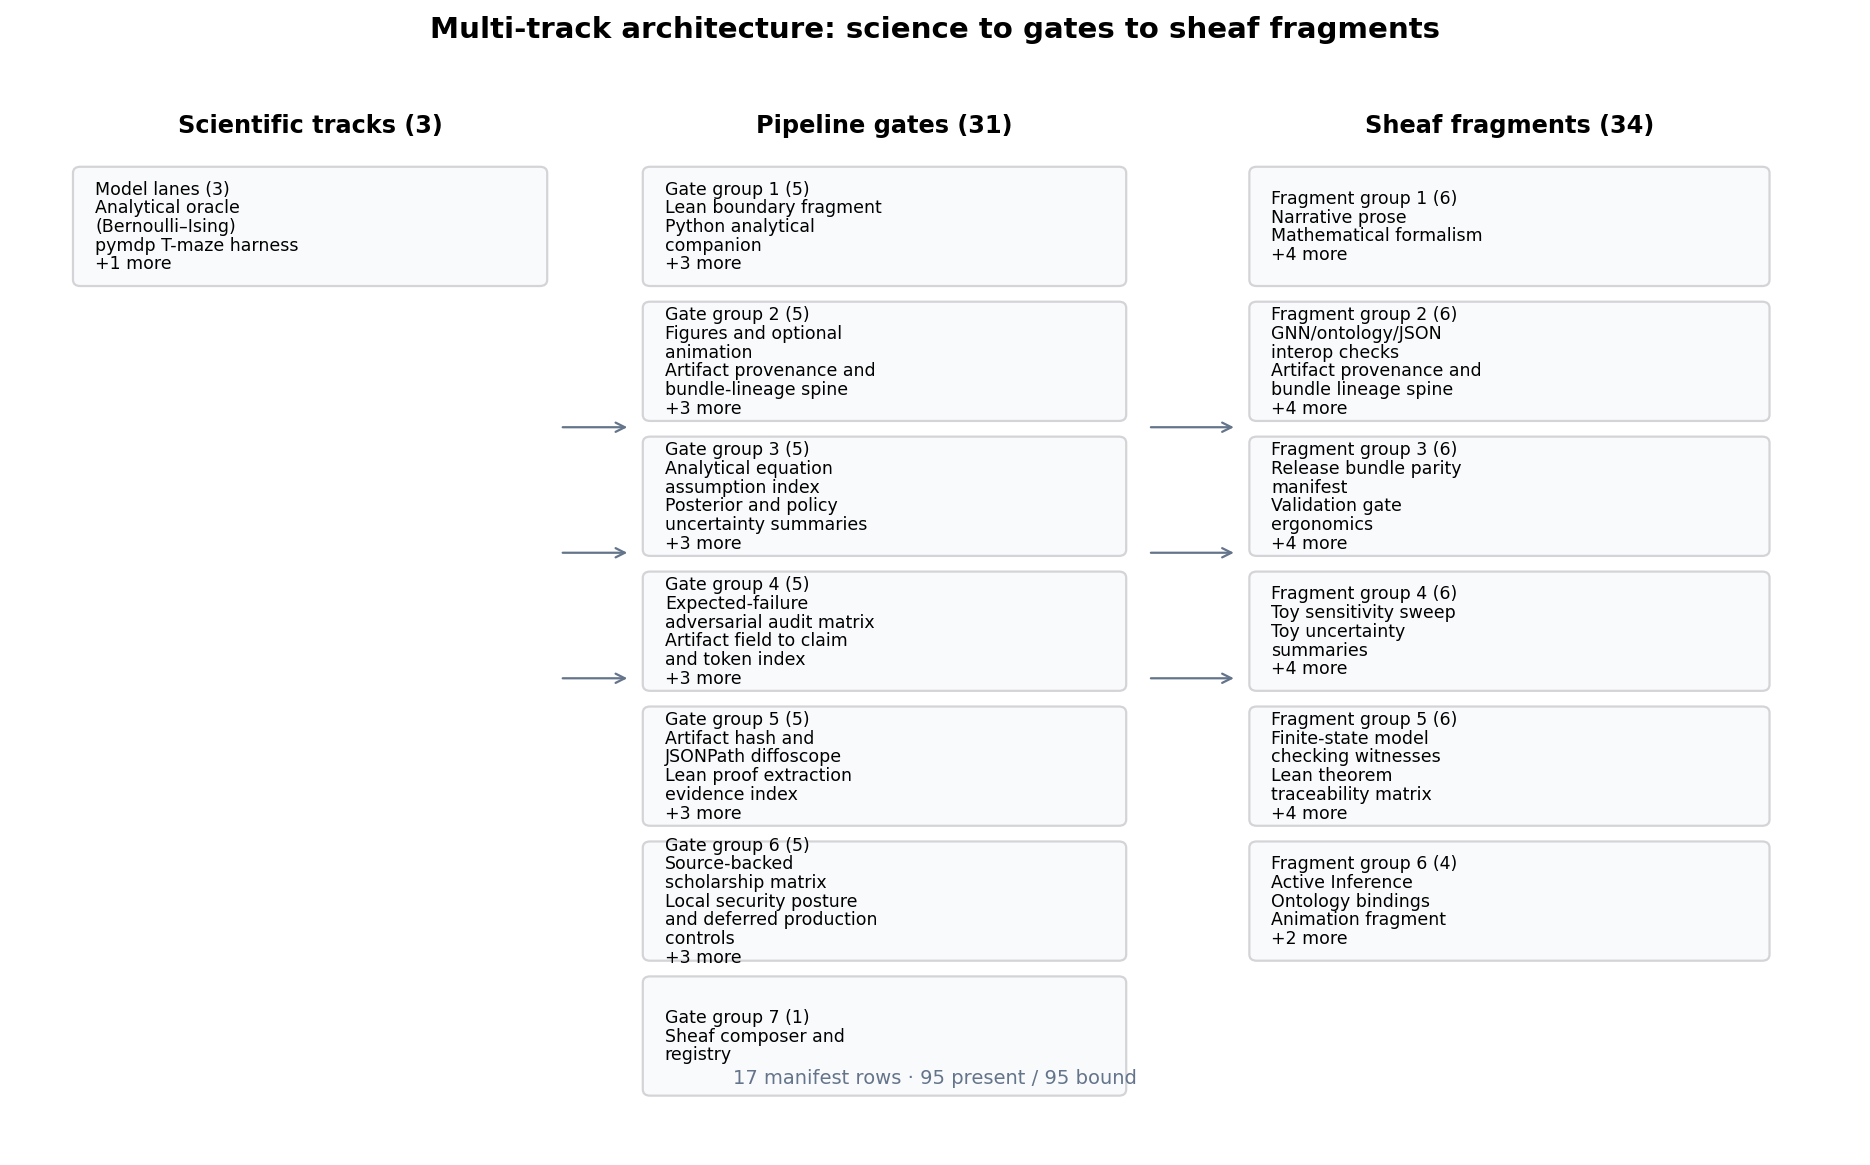
\includegraphics[width=0.95\linewidth,height=0.5\textheight,keepaspectratio,alt={Multi-track architecture: analytical, pymdp, and sheaf composition lanes mapped to 31 pipeline gates and 34 composable fragment types.}]{../figures/multi_track_architecture.png}
\caption{Multi-track architecture: analytical, pymdp, and sheaf
composition lanes mapped to 31 pipeline gates and 34 composable fragment
types.}\label{fig:multi_track_architecture}
\end{figure}

\subsubsection{Ontology bindings}\label{ontology-bindings}

\begin{itemize}
\tightlist
\item
  \breaktt{expected\_free\_energy} \texorpdfstring{\ensuremath{\to}}{->} \textbf{ExpectedFreeEnergy}
\item
  \texttt{location} \texorpdfstring{\ensuremath{\to}}{->} \textbf{HiddenState}
\item
  \texttt{observation} \texorpdfstring{\ensuremath{\to}}{->} \textbf{ObservationLikelihood}
\item
  \texttt{policy} \texorpdfstring{\ensuremath{\to}}{->} \textbf{PolicyPosterior}
\end{itemize}

\newpage

\phantomsection
\addcontentsline{toc}{section}{Methods}
\section*{Methods}

\section{Bernoulli--Ising analytical
model}\label{sec:methods_analytical}

The analytical method is a finite \textbf{K=2 Bernoulli / Ising} oracle.
The entangled joint eq.~\ref{eq:entangled_joint} gives closed-form
mutual information \(I(\lambda)\);
\breaktt{output/data/parameter\_sweep.csv} then checks the same curve by
an independent exact total-correlation recomputation before the value is
used in sec.~\ref{sec:results_mi_sweep}. GNN and ontology rows share the
same symbol surface (fig.~\ref{fig:gnn_ontology_concordance}), so the
derivation, sweep, and model notation are one audited toy contract
rather than parallel descriptions.

The scope is intentionally small: finite variational quantities only, no
sampling, and no empirical generalization. ``Free energy'' here means
exactly computed variational functionals on this tiny discrete
state-space, aligned with mathematical FEP reviews
\citep{buckley2017mathreview}, not continuous-time or biological FEP
dynamics \citep{gershman2019fepbrain}. The generated sweep contains 21
grid points, and the merged invariant report records 12 / 12 passing
checks.

The entangled joint over binary policies satisfies

\begin{equation}\protect\phantomsection\label{eq:entangled_joint}{
q_\lambda(\pi) \propto E(\pi)\,\exp(\lambda J(\pi)),
}\end{equation}

with symmetric Ising coupling \(J\) and deformation parameter
\(\lambda\). Let \(\sigma(\lambda)=q_\lambda(\pi_1=\pi_2)\) be the
probability that the two streams agree (the diagonal mass of the
\(2\times2\) joint); by symmetry both marginals are uniform. With binary
entropy \(H_b(p)=-p\log p-(1-p)\log(1-p)\) in nats, the joint entropy is
\(H(q_\lambda)=\log 2 + H_b(\sigma(\lambda))\) while each marginal
contributes \(\log 2\), so the mutual information is

\[
I(\lambda)=\sum_k H(q_k)-H(q_\lambda)=\log 2 - H_b(\sigma(\lambda)),
\]

vanishing at \(\lambda=0\) (\(\sigma=\tfrac12\), independent streams)
and saturating at \(\log 2\) as \(\lambda\to\infty\) (\(\sigma\to1\),
perfectly entangled). These symbols are the rows of
\breaktt{analytical\_assumption\_index.json}, so the derivation is
auditable rather than asserted.

The analytical track writes a parameter sweep comparing closed-form
mutual information with an independent exact recomputation of it (via
total correlation) across \(\lambda \in [0, 4]\) on 21 grid points
(sec.~\ref{sec:results_mi_sweep}, fig.~\ref{fig:ising_mi_curve}).

The \breaktt{assumption\_index} fragment makes the analytical equations
inspectable as a generated artifact instead of relying on prose labels.
\breaktt{output/data/analytical\_assumption\_index.json} indexes 7
finite-model equation identifiers and 7 rows; the hydrated pass flag is
\texttt{true}.

The index is deliberately narrow. It covers the Bernoulli-Ising toy
equations, their finite binary state assumptions, and the generated
artifacts that test the same symbols. Any missing equation identifier or
empty assumption list fails the toy-sweep validation gate.

\begin{figure}
\centering
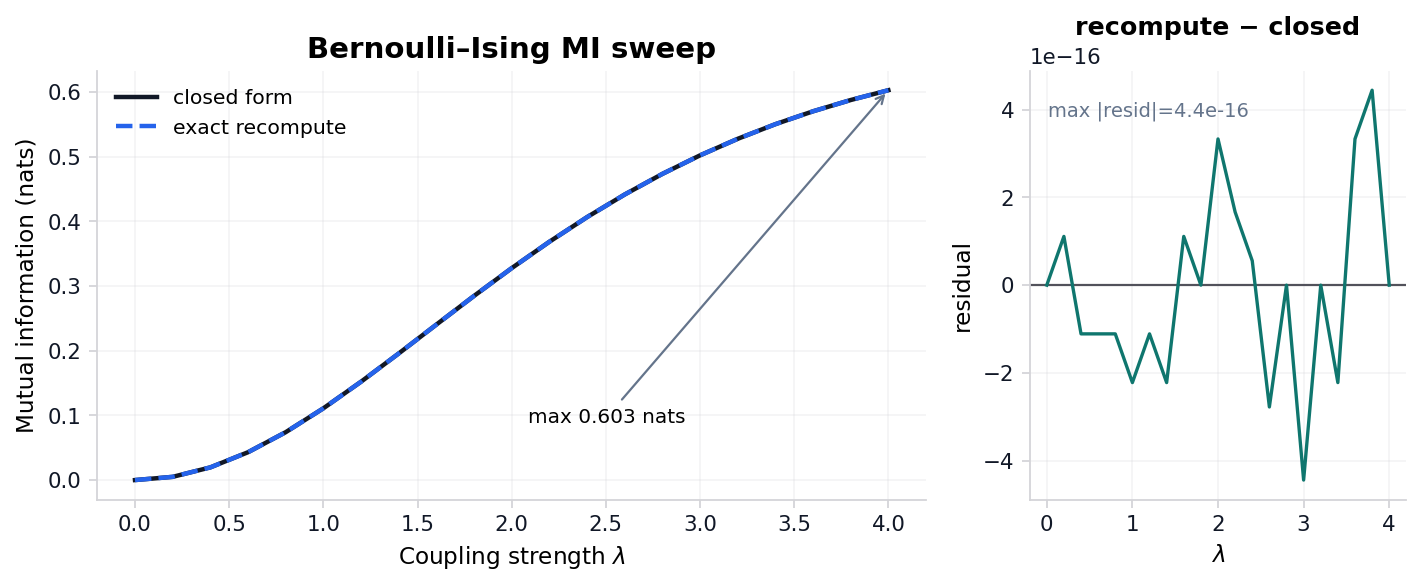
\includegraphics[width=0.9\linewidth,height=0.5\textheight,keepaspectratio,alt={Closed-form I(\textbackslash lambda) and an independent exact recomputation via total correlation for the symmetric Bernoulli-Ising toy across 21 grid points up to \textbackslash lambda\_\{\textbackslash max\} = 4; grid maximum 0.6031 nats. Both estimators are deterministic (no sampling), so the right panel is a cross-implementation agreement check (max residual 0 nats), not a sampling residual.}]{../figures/ising_mi_curve.png}
\caption{Closed-form \(I(\lambda)\) and an independent exact
recomputation via total correlation for the symmetric Bernoulli-Ising
toy across 21 grid points up to \(\lambda_{\max}\) = 4; grid maximum
0.6031 nats. Both estimators are deterministic (no sampling), so the
right panel is a cross-implementation agreement check (max residual 0
nats), not a sampling residual.}\label{fig:ising_mi_curve}
\end{figure}

\begin{figure}
\centering
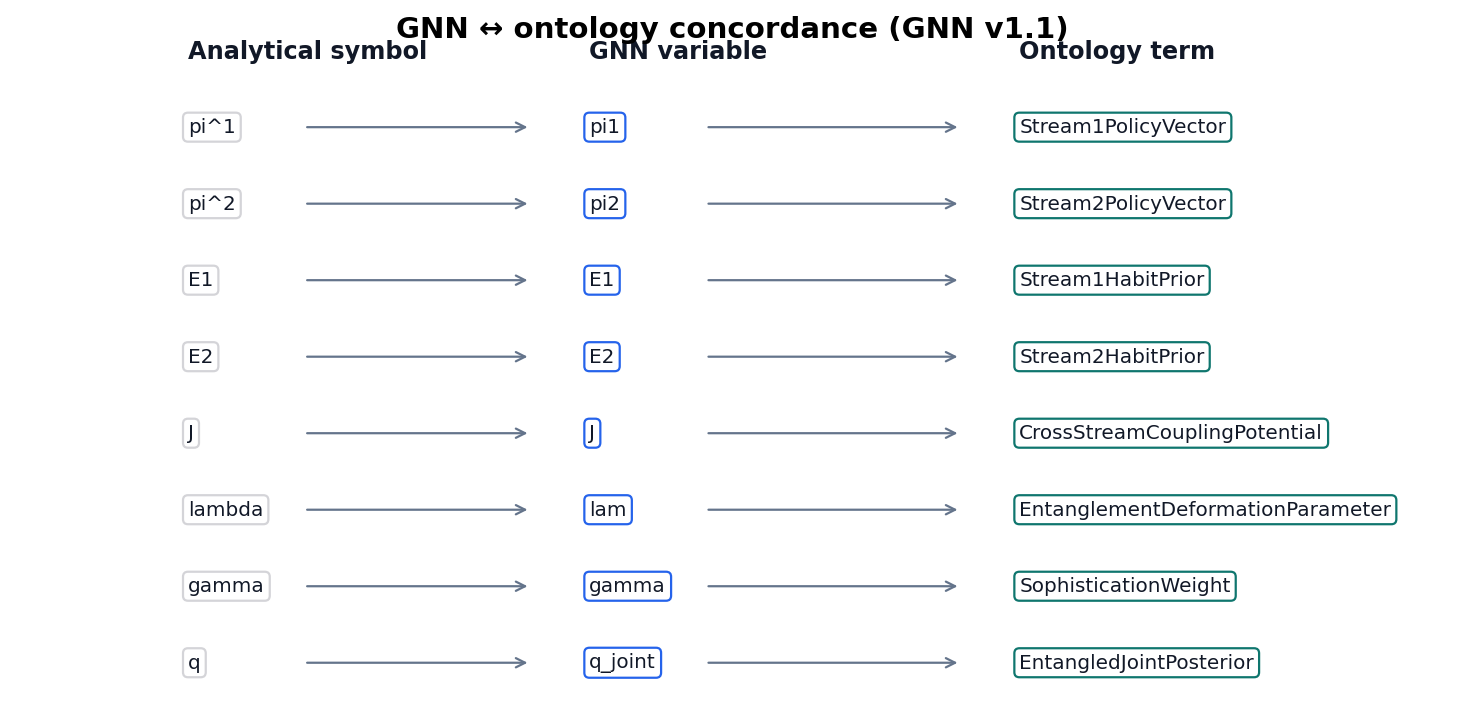
\includegraphics[width=0.9\linewidth,height=0.5\textheight,keepaspectratio,alt={GNN \textbackslash leftrightarrow ontology concordance for the Bernoulli--Ising toy (GNN v1.1).}]{../figures/gnn_ontology_concordance.png}
\caption{GNN \(\leftrightarrow\) ontology concordance for the
Bernoulli--Ising toy (GNN v1.1).}\label{fig:gnn_ontology_concordance}
\end{figure}

The Bernoulli toy is declared in \breaktt{gnn/bernoulli\_toy.gnn.md} (GNN
v1.1), following the GNN notation role described by Smekal and Friedman
\citep{gnn2023}. fig.~\ref{fig:gnn_ontology_concordance} links GNN
variables to Active Inference Ontology terms bound in the analytical
ontology fragment; round-trip parity is checked before render.

Measured MI and sweep artifacts in sec.~\ref{sec:results_mi_sweep}
ground the same symbol map used in the concordance diagram.

\subsubsection{Ontology bindings}\label{ontology-bindings-1}

\begin{itemize}
\tightlist
\item
  \texttt{E1} \texorpdfstring{\ensuremath{\to}}{->} \textbf{Stream1HabitPrior}
\item
  \texttt{E2} \texorpdfstring{\ensuremath{\to}}{->} \textbf{Stream2HabitPrior}
\item
  \texttt{J} \texorpdfstring{\ensuremath{\to}}{->} \textbf{CrossStreamCouplingPotential}
\item
  \texttt{gamma} \texorpdfstring{\ensuremath{\to}}{->} \textbf{SophisticationWeight}
\item
  \texttt{lam} \texorpdfstring{\ensuremath{\to}}{->} \textbf{EntanglementDeformationParameter}
\item
  \texttt{pi1} \texorpdfstring{\ensuremath{\to}}{->} \textbf{Stream1PolicyVector}
\item
  \texttt{pi2} \texorpdfstring{\ensuremath{\to}}{->} \textbf{Stream2PolicyVector}
\item
  \texttt{q\_joint} \texorpdfstring{\ensuremath{\to}}{->} \textbf{EntangledJointPosterior}
\end{itemize}

\newpage

\section{pymdp simulation harness}\label{sec:methods_pymdp}

\textbf{Sophisticated inference (planning horizon).} The pymdp method is
a deterministic state-inference harness on a minimal T-maze
(fig.~\ref{fig:tmaze_schematic}) with planning horizon
\breaktt{policy\_len\ =\ 2}. The discrete-state framing follows finite
POMDP active-inference treatments and sophisticated-inference analyses
\citep{dacosta2020discrete, smith2022tutorial, friston2021sophisticated, dacosta2023reward},
and the implementation anchor is the pymdp software paper
\citep{pymdp2024}. The default \texttt{state\_inference} rollout writes
the summary/trace artifacts used in sec.~\ref{sec:results_si_tmaze};
mean belief entropy is 0.3251.

The method keeps runtime, posterior, and extension evidence separate.
\breaktt{output/data/si\_policy\_comparison.json} compares
\texttt{state\_inference} and \breaktt{policy\_inference} over declared
toy horizons and seeds without replacing the default rollout (4 rows;
complete-grid flag 1). Agent construction and backend warnings live in
\breaktt{output/reports/pymdp\_runtime\_diagnostics.json} (4
constructions, 4 known third-party warnings, 0 unexpected warnings).
Posterior rows live in
\breaktt{output/data/pymdp\_policy\_posterior\_grid.json} and must remain
normalized (\texttt{1}).

Graph-world artifacts are deterministic extension outputs declared in
\texttt{tracks.yaml} rather than new empirical claims.
\breaktt{simulate\_si\_graph\_world.py} writes summary and trace
artifacts for the finite graph path; the regenerated summary reports 4
nodes, 4 steps, and goal-reached flag 1. The topology-trace extension
records 4 toy topology traces with agreement flag 1.

Given generative matrices \(A,B,C,D\), pymdp computes state beliefs
\(q(s)\) via variational inference (\texttt{infer\_states}). The Agent
is configured with planning horizon \(H =\) 2, which defines the
\textbf{policy depth} used when constructing candidate policies (logged
as \texttt{num\_policies} in the SI summary artifact; see
sec.~\ref{sec:results_si_tmaze}).

The default harness records belief entropy per step; extending to full
expected-free-energy policy selection (\texttt{infer\_policies}) is
documented as a follow-on track in sec.~\ref{sec:discussion_outlook}.

SI artifacts (summary, trace, optional JSONL log) record step count,
actions, observations, and belief entropy for
sec.~\ref{sec:results_si_tmaze}. Steps recorded: 2. Branching-time and
variational formulations of active inference planning are treated here
as related planning context
\citep{champion2021branching, nuijten2026efeplanning}; the live evidence
remains the finite local artifacts \breaktt{si\_policy\_grid.json},
\breaktt{si\_efe\_terms.json}, and
\breaktt{model\_checking\_witnesses.json}, not a claim about scalable
planning performance.

The \texttt{interop} fragment treats the GNN files, JSON views, and
ontology bindings as a round-trip contract rather than parallel
documentation. \breaktt{output/data/interop\_roundtrip\_report.json}
records 2 deterministic checks; the manuscript only claims losslessness
when \texttt{true} is true.

The stricter lint artifacts are adjacent evidence, not new model claims:
\breaktt{output/data/gnn\_roundtrip\_report.json},
\breaktt{output/reports/gnn\_lint\_report.json},
\breaktt{output/data/ontology\_alias\_index.json}, and
\breaktt{output/data/ontology\_profile\_matrix.json} must agree before
the interop row passes. A missing GNN variable, duplicate ontology
alias, dropped JSON field, shape diff, or dtype diff is therefore a
validation failure before rendering.

\begin{figure}
\centering
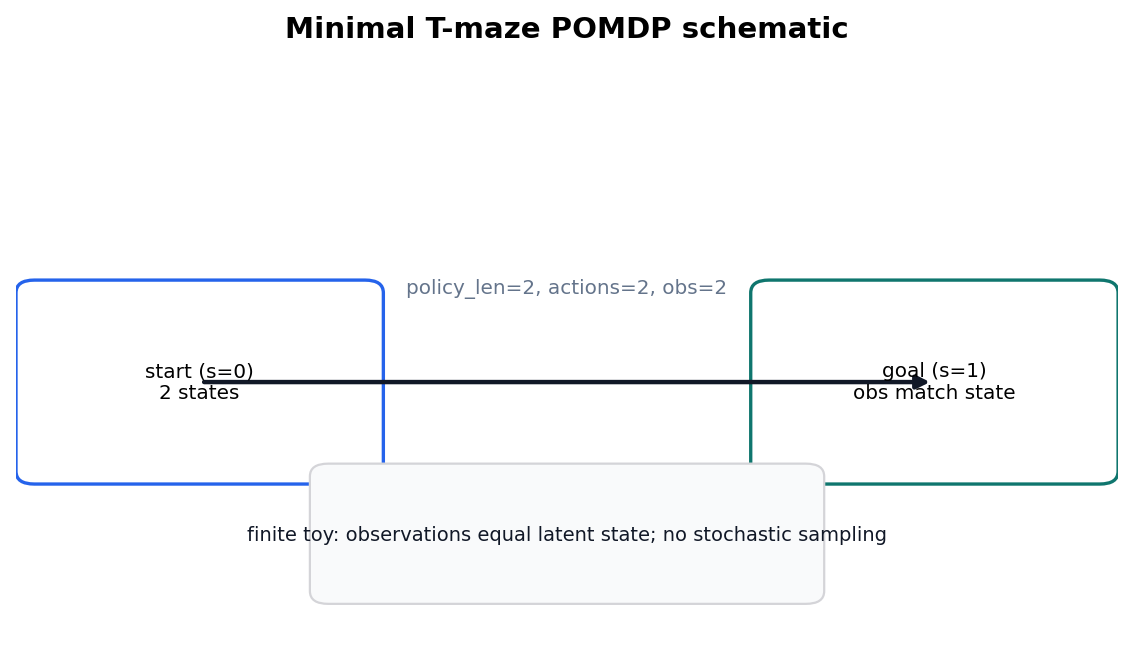
\includegraphics[width=0.85\linewidth,height=0.5\textheight,keepaspectratio,alt={T-maze generative model schematic (2-step policy horizon, state\_inference mode).}]{../figures/tmaze_schematic.png}
\caption{T-maze generative model schematic (2-step policy horizon,
state\_inference mode).}\label{fig:tmaze_schematic}
\end{figure}

See \breaktt{gnn/si\_tmaze.gnn.md} for a GNN view of the T-maze hidden
state, observation, and policy variables with ontology bindings.

\subsubsection{Ontology bindings}\label{ontology-bindings-2}

\begin{itemize}
\tightlist
\item
  \texttt{belief\_entropy} \texorpdfstring{\ensuremath{\to}}{->} \textbf{BeliefEntropy}
\item
  \texttt{loc} \texorpdfstring{\ensuremath{\to}}{->} \textbf{HiddenState}
\item
  \texttt{obs} \texorpdfstring{\ensuremath{\to}}{->} \textbf{ObservationLikelihood}
\item
  \texttt{pi} \texorpdfstring{\ensuremath{\to}}{->} \textbf{PolicyPosterior}
\end{itemize}

\newpage

\section{Lean formalization boundary}\label{sec:methods_lean}

The Lean method is a boundary witness track, not a broad formalization
of active inference. \texttt{lake\ build} checks declarations under
\breaktt{lean/TemplateActiveInference/};
fig.~\ref{fig:lean_boundary_status} renders the proved/deferred surface,
while generated inventories carry theorem names, constructive-token
status, and axiom checks.

The theorem set links back to the finite analytical and pymdp toys.
Horizon witnesses constrain the planning-depth examples, and
\breaktt{efe\_additive\_identity\_from\_relations} proves
\breaktt{(risk\ +\ ambiguity)\ +\ (pragmatic\ +\ epistemic)\ =\ 0} from
the definitional relations using core integer arithmetic
(\texttt{omega}). These rows join 17 linked theorem-traceability entries
with all-linked flag \texttt{true}; no prose claim is promoted unless
the generated theorem, witness, and evidence-field rows agree.

\begin{figure}
\centering
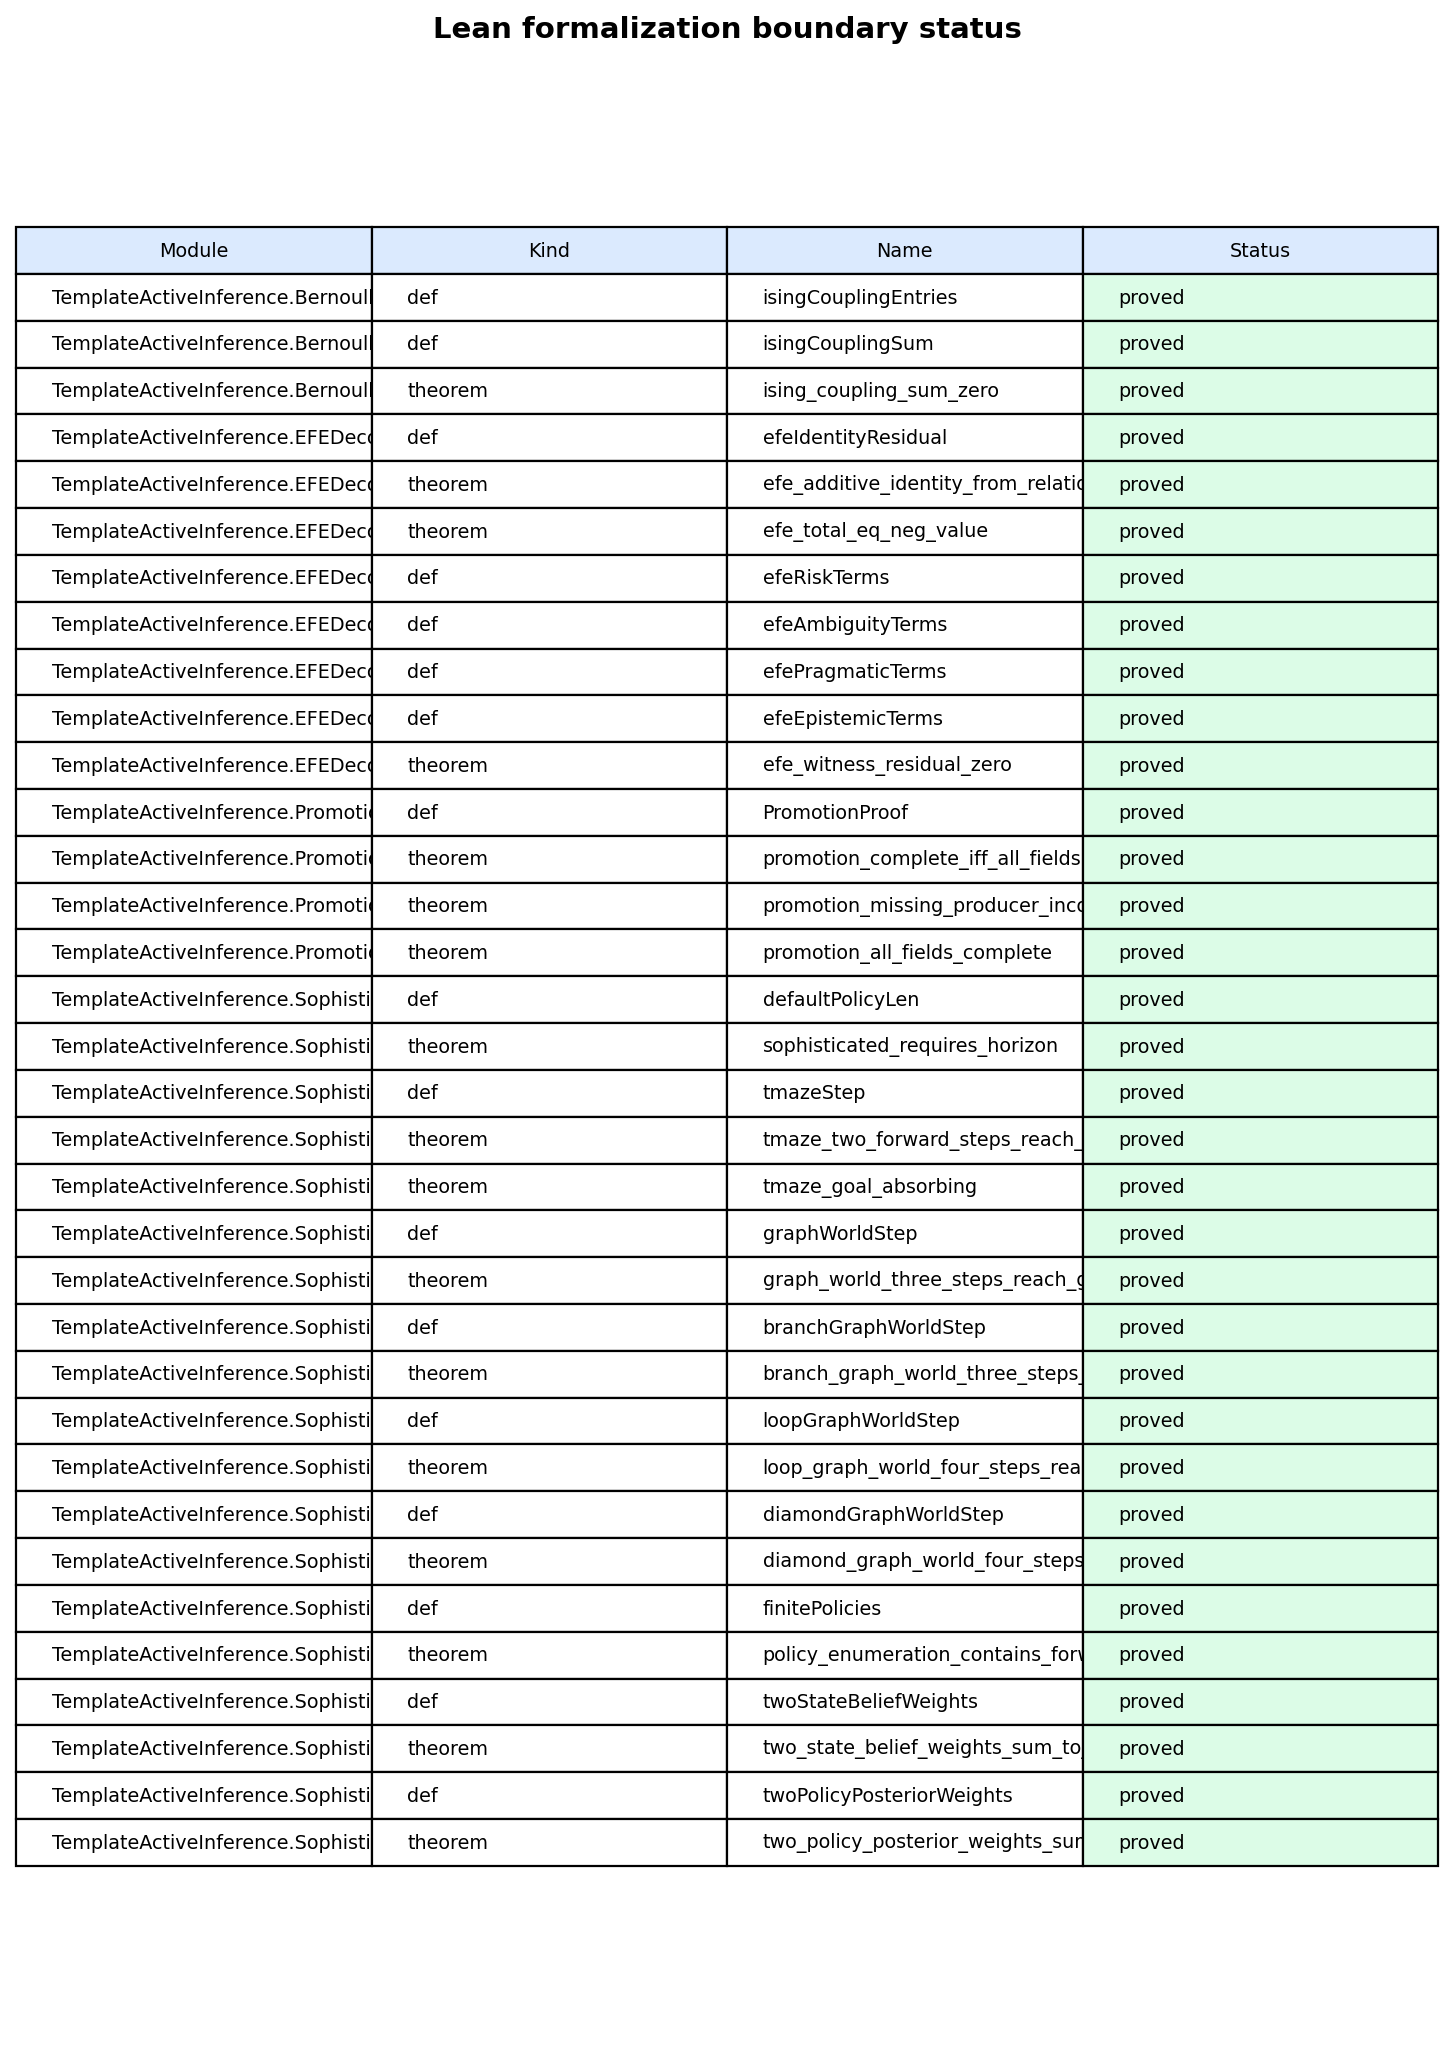
\includegraphics[width=0.9\linewidth,height=0.5\textheight,keepaspectratio,alt={Lean formalization boundary: module witnesses checked by lake build.}]{../figures/lean_boundary_status.png}
\caption{Lean formalization boundary: module witnesses checked by lake
build.}\label{fig:lean_boundary_status}
\end{figure}

Lean module \breaktt{TemplateActiveInference.SophisticatedInference}
declares the planning-horizon parameter \breaktt{defaultPolicyLen} and
finite T-maze boundary witnesses:
\texttt{sophisticated\_requires\_horizon\ :\ defaultPolicyLen\ \textgreater{}\ 1},
\breaktt{tmaze\_two\_forward\_steps\_reach\_goal}, and
\breaktt{tmaze\_goal\_absorbing}. It also contains constructive finite
witnesses for graph-world reachability, finite policy enumeration,
two-state belief weights, and two-policy posterior weights. These
theorems formalize small finite boundaries shared with generated
artifacts; they do \emph{not} prove that the toy policy posterior is a
general model of sophisticated inference. Axioms are audited with
\texttt{\#print\ axioms} (the gate whitelists only \texttt{propext},
\breaktt{Classical.choice}, \texttt{Quot.sound}); see the Lean track
gate.

Build via \texttt{lake\ build} under \texttt{lean/}.

The \texttt{model\_checking} fragment complements Lean with finite
exhaustive witnesses.
\breaktt{output/reports/model\_checking\_witnesses.json} records 12
toy-state witnesses and reports \texttt{true} only when no
counterexample is found in the enumerated state/action space.

This is deliberately narrower than a semantic proof of all Active
Inference programs. It checks the finite T-maze and graph-world boundary
objects used by this manuscript and exposes the witness inventory to the
same artifact and claim gates as the Lean theorem inventory. The Lean
graph-world inventory witnesses 4 generated toy topology ids, with
all-topologies-witnessed flag \texttt{true}; theorem traceability
contributes 17 linked rows.

The \breaktt{theorem\_traceability} fragment binds Lean theorem inventory
rows to finite model-checking witnesses, manuscript claims, and evidence
fields. \breaktt{output/data/theorem\_traceability\_matrix.json} records
17 traceability rows and passes only when every theorem row is linked
(\texttt{true}).

\subsubsection{Proof extraction track}\label{proof-extraction-track}

The \breaktt{proof\_extraction} track extracts Lean theorem statements
and proof-source metadata into
\breaktt{output/data/proof\_extraction\_index.json}. The index currently
contains 12 extracted theorem rows, with constructive-token status
\texttt{true}.

\newpage

\section{Sheaf composition}\label{sec:methods_sheaf}

\subsection{Compose contract}\label{compose-contract}

Each manifest row in \breaktt{manuscript/sheaf/manifest.yaml} binds
fragment tracks from \breaktt{manuscript/sheaf/tracks.yaml}. A track
supplies a renderer, compose order, label, optional flag, general paper
role, and paper-specific use statement; the composer then flattens the
binding set into one Markdown section for PDF and web output.

The operational claim is auditable binding. Analytical, simulation,
pymdp, visualization, Lean, GNN, ontology, scholarship, and optional
media fragments attach to IMRAD rows under eq.~\ref{eq:coverage_cell}
(\textbf{P} present, \textbf{---} unbound, \textbf{M} missing). This is
an applied local-to-global consistency contract in the spirit of
cellular sheaf and sheaf-signal-processing work
\citep{curry2014sheaves, robinson2014topological}, instantiated here as
a finite artifact gate rather than a cohomology claim.

\subsection{Coverage and figures}\label{coverage-and-figures}

fig.~\ref{fig:sheaf_layers_overview} summarizes 34 fragment types and
their IMRAD bindings. Generated tables below list every track definition
and section\texorpdfstring{\ensuremath{\times}}{x}track binding at compose time. The visualization track is
gated by \breaktt{output/reports/visualization\_quality\_audit.json}: 23
/ 23 registered figures render, 23 are source-mapped, and 23 have
sufficient alt/caption metadata; the all-quality flag is \texttt{true}.

The visualization gate is deliberately row-level. It requires declared
visual/evidence roles (\texttt{true}), artifact-backed paper claims
(\texttt{true}), section bindings (\texttt{true}), RGB nonblank image
renders, hashes, and source-map agreement. The statistical bridge then
expands 7 statistically backed figures into 7 figure-source-scholarship
rows with connected status \texttt{true}, manuscript-reference status
\texttt{true}, and visualization-bound reference status \texttt{true}.

The claim ledger is also checked at row level rather than as prose
metadata. \breaktt{claim\_evidence\_audit.json} resolves 97 claim rows to
live artifacts (\texttt{true}) and replays their typed predicates
(\texttt{true}), yielding the promoted completeness flag \texttt{true}.

\subsection{Compose commands}\label{compose-commands}

\begin{Shaded}
\begin{Highlighting}[]
\ExtensionTok{uv}\NormalTok{ run python scripts/compose\_manuscript.py}
\ExtensionTok{uv}\NormalTok{ run python scripts/compose\_manuscript.py }\AttributeTok{{-}{-}validate{-}only} \AttributeTok{{-}{-}strict}
\end{Highlighting}
\end{Shaded}

Each run emits \breaktt{output/data/sheaf\_coverage\_matrix.json} and
regenerates coverage artifacts. Partial compose (\texttt{-\/-section})
is draft-only; the matrix always reflects the full manifest. Coverage
totals appear on sec.~\ref{sec:sheaf_coverage}; discussion scope is in
sec.~\ref{sec:discussion_outlook}.

\subsection{Law verification}\label{law-verification}

\breaktt{-\/-validate-only\ -\/-strict} runs the structural gate before
any fragment is glued. Beyond per-cell coverage, it invokes the
sheaf-law oracle (\breaktt{verify\_sheaf\_laws},
\breaktt{src/manuscript/sheaf/laws.py}), which checks 6 axioms --- poset,
presheaf functoriality, separation, gluing, typing, and compositionality
--- and reports 6/6 satisfied for the current manifest. A violation is
raised as an error-level issue and aborts the build, so a malformed
manifest (a section colliding on an output file, an off-chain block, a
mistyped fragment, a fragment shared between sections) can never
compose. The formal statements are in the formalism block below; the
negative-control suite (\breaktt{tests/test\_sheaf\_laws.py}) proves each
check is falsifiable.

The semantic layer is separate from those structural laws.
\breaktt{output/data/sheaf\_gluing\_certificate.json} records cross-track
symbols, typed claim evidence, artifact sources, and manuscript-variable
restrictions; validation fails when the analytical, pymdp, GNN,
ontology, Lean, visualization, or manuscript tracks disagree about a
shared symbol or measured claim. The visualization-quality audit is one
of those restrictions, so a missing source map, missing statistical
bridge source, missing hash, blank render, non-RGB render, undersized
figure, or unbound section breaks the same semantic contract that checks
statistics and theorem witnesses. fig.~\ref{fig:semantic_gluing_graph}
renders the configured producers, generated evidence artifacts, and
validation consumers that read each shared symbol.

\subsubsection{Base poset and presheaf}\label{base-poset-and-presheaf}

The manuscript is modelled as a coverage sheaf over a finite base poset.
Let the \textbf{base} \(P\) be the IMRAD blocks ordered as a chain,

\begin{equation}\protect\phantomsection\label{eq:imrad_chain}{
\mathsf{Introduction} \prec \mathsf{Methods} \prec \mathsf{Results} \prec \mathsf{Discussion} \prec \mathsf{Appendix},
}\end{equation}

with, in each block, a \emph{group} node above its \emph{section} nodes
(written \(G \sqsupseteq s\)). \(P\) is therefore a finite poset
(equivalently a finite Alexandrov space). Let \(\mathcal{T}\) be the
registered fragment-track set from
\breaktt{manuscript/sheaf/tracks.yaml}; each track \(t \in \mathcal{T}\)
carries a renderer \(R(t)\), label \(L(t)\), optional flag \(O(t)\), a
general paper role \(U(t)\), a section-use statement \(V(t)\), and a
strict compose-order index \(\pi(t)\).

The \textbf{presheaf} \(\mathcal{F}\) is a contravariant functor on
\(P\) --- \(\mathcal{F}\colon P \to \mathbf{Set}\) with restriction maps
along \(\sqsupseteq\) --- assigning to each composing section \(s\) its
bound fragment set
\(\mathcal{F}(s) = \{\,(t, F_s(t)) : t \text{ bound in } s\,\}\), where
\(F_s : \mathcal{T} \rightharpoonup \mathbf{Path}\) is the section's
partial binding map. Restriction along \(G \sqsupseteq s\) is projection
onto a section's own bindings; group nodes carry the empty assignment
and do not compose.

The coverage cell is

\begin{equation}\protect\phantomsection\label{eq:coverage_cell}{
B(s,t) \in \{\mathrm{P}, \mathrm{—}, \mathrm{M}\}
}\end{equation}

derived from \(F_s(t)\) and filesystem existence at compose time:
\textbf{P} when a bound fragment exists, \textbf{---} when the track is
unbound for that row, and \textbf{M} when a bound path is missing. The
current regenerated matrix reports 95 present / 95 bound / 0 missing
cells. Registry size: \(|\mathcal{T}| = 34\) types across 17 IMRAD
manifest rows (5 group rows, 12 composing sections).

\subsubsection{Verified sheaf laws}\label{verified-sheaf-laws}

What makes this presheaf a \emph{sheaf} --- rather than a bare incidence
table --- is that the composer's structural axioms are machine-checked.
The oracle \breaktt{verify\_sheaf\_laws}
(\breaktt{src/manuscript/sheaf/laws.py}) verifies 6 laws, and the
regenerated build reports 6/6 satisfied:

\begin{enumerate}
\def\labelenumi{\arabic{enumi}.}
\tightlist
\item
  \textbf{Poset.} The IMRAD blocks form the chain of
  eq.~\ref{eq:imrad_chain}; compose order is monotone in block rank and
  every composing section's block carries a group row.
\item
  \textbf{Presheaf (functoriality).} Every bound track lies in
  \(\mathcal{T}\); \(\pi\) is a strict total order; and each section's
  resolved track order is the monotone restriction of \(\pi\) (an
  explicit \texttt{track\_order} override must be a permutation of the
  section's bound tracks).
\item
  \textbf{Separation (locality).} The map
  \(s \mapsto \mathrm{output\_name}(s)\) is injective over composing
  sections: distinct locals glue to distinct global positions, so the
  global section is unique.
\item
  \textbf{Gluing.} Compose order is a linear extension of \(P\) --- each
  block's rows are contiguous and strictly increasing in order --- so
  the local fragments glue to a unique global manuscript in which every
  composing section appears exactly once.
\item
  \textbf{Typing.} Each binding \((t, F_s(t))\) is well-typed: \(R(t)\)
  is a registered renderer and the fragment suffix lies in \(R(t)\)'s
  accepted suffix set. Generated renderers (\texttt{section\_figures},
  \texttt{layers\_report}) synthesize their body and are explicitly
  type-exempt.
\item
  \textbf{Compositionality.} Every fragment file is private to one
  section (no path is bound twice), so global composition is the
  coproduct of the per-section bodies and is independent of inclusion
  order.
\end{enumerate}

Each law is paired with a negative control in
\breaktt{tests/test\_sheaf\_laws.py} --- a single mutation that breaks
the law and is proven to be caught --- so the gate binds the laws'
\emph{content}, not merely their shape. Under \texttt{-\/-strict}, any
violation is surfaced as an error-level manifest issue and aborts
composition.

\subsubsection{Scope (what is and is not
claimed)}\label{scope-what-is-and-is-not-claimed}

These laws verify the sheaf \emph{axioms} on a finite base poset. They
do \textbf{not} compute sheaf \emph{cohomology} (\(H^0\)/\(H^1\), Čech
complexes, derived functors); ``sheaf'' here names the verified
separation-and-gluing structure of a multi-track coverage assignment,
not a cohomological invariant. Formal track definitions and
section\texorpdfstring{\ensuremath{\times}}{x}track bindings appear in the generated tables below.

Semantic gluing then checks agreement of the glued content: coverage
counts, manuscript variables, typed claim predicates, pymdp mode/hash,
Bernoulli GNN ontology, and SI T-maze GNN ontology. This certificate is
a content-level audit over the same base, not an additional topological
law.

\begin{figure}
\centering
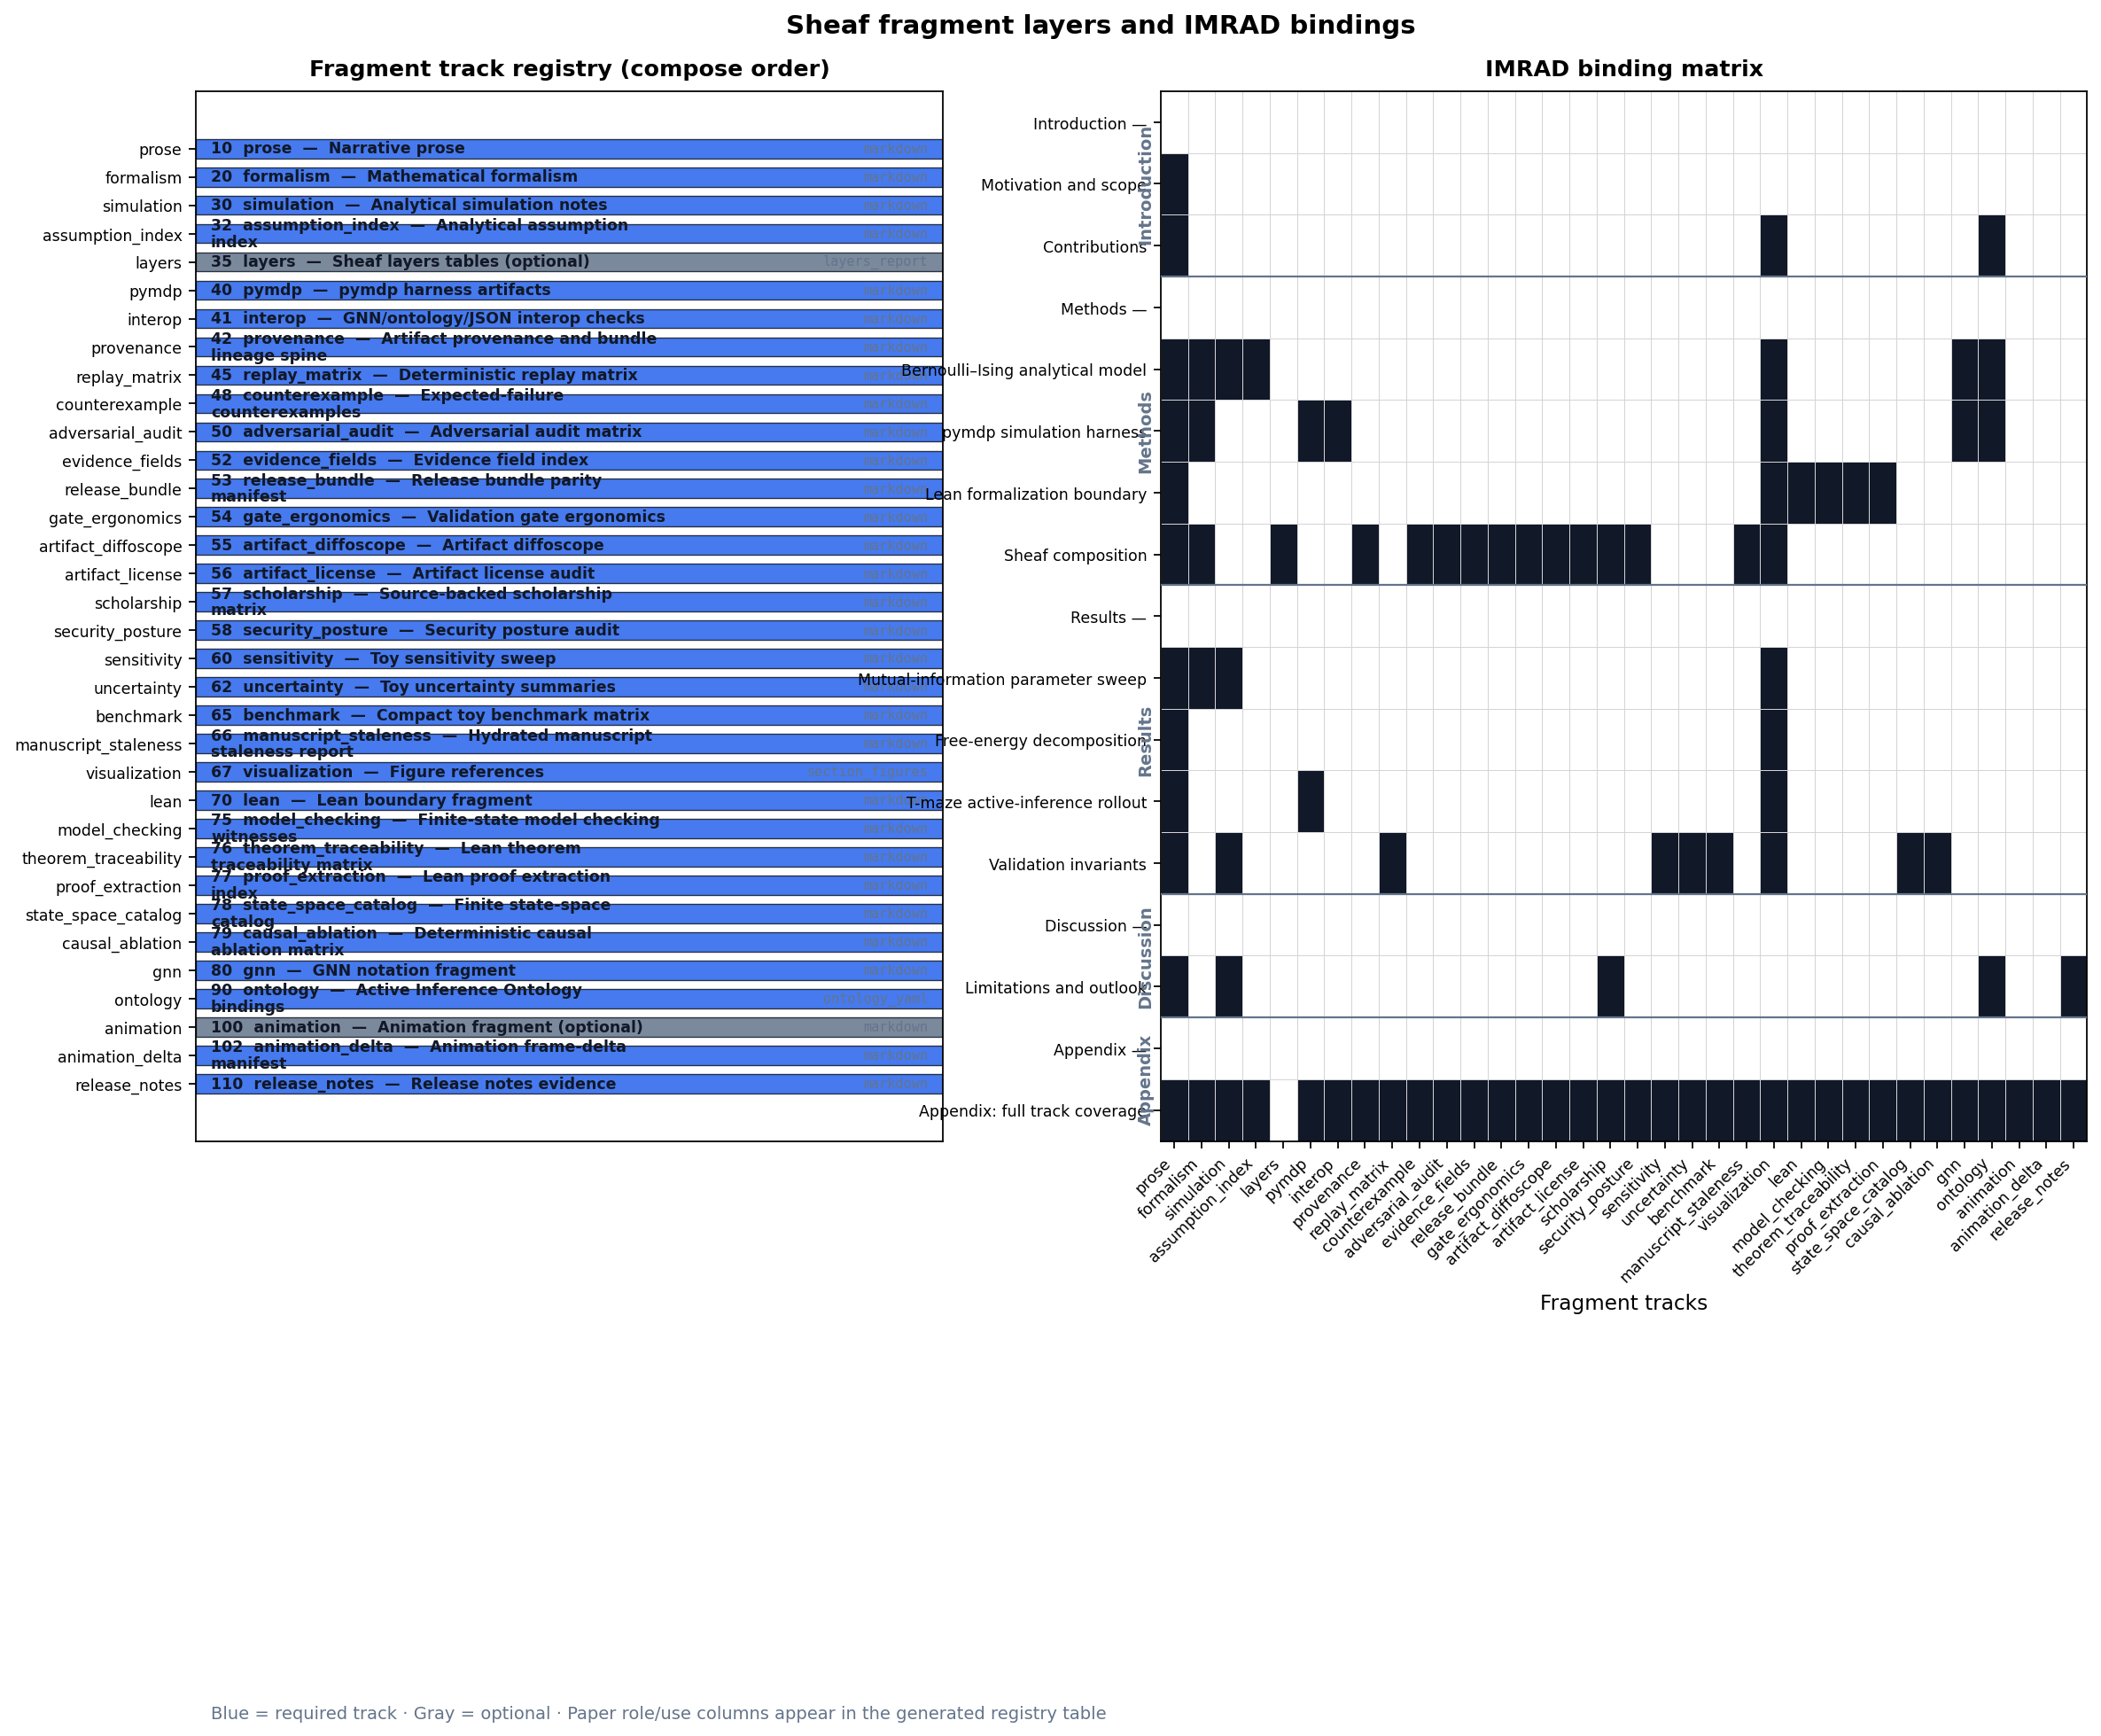
\includegraphics[width=0.98\linewidth,height=0.5\textheight,keepaspectratio,alt={Sheaf layers overview: registry stack (compose order, renderer ids) and IMRAD binding heatmap for 34 fragment types across 17 manifest rows (95 present / 95 bound / 0 missing), generated from output/data/sheaf\_coverage\_matrix.json.}]{../figures/sheaf_layers_overview.png}
\caption{Sheaf layers overview: registry stack (compose order, renderer
ids) and IMRAD binding heatmap for 34 fragment types across 17 manifest
rows (95 present / 95 bound / 0 missing), generated from
\protect\breaktt{output/data/sheaf\_coverage\_matrix.json}.}\label{fig:sheaf_layers_overview}
\end{figure}

\begin{figure}
\centering
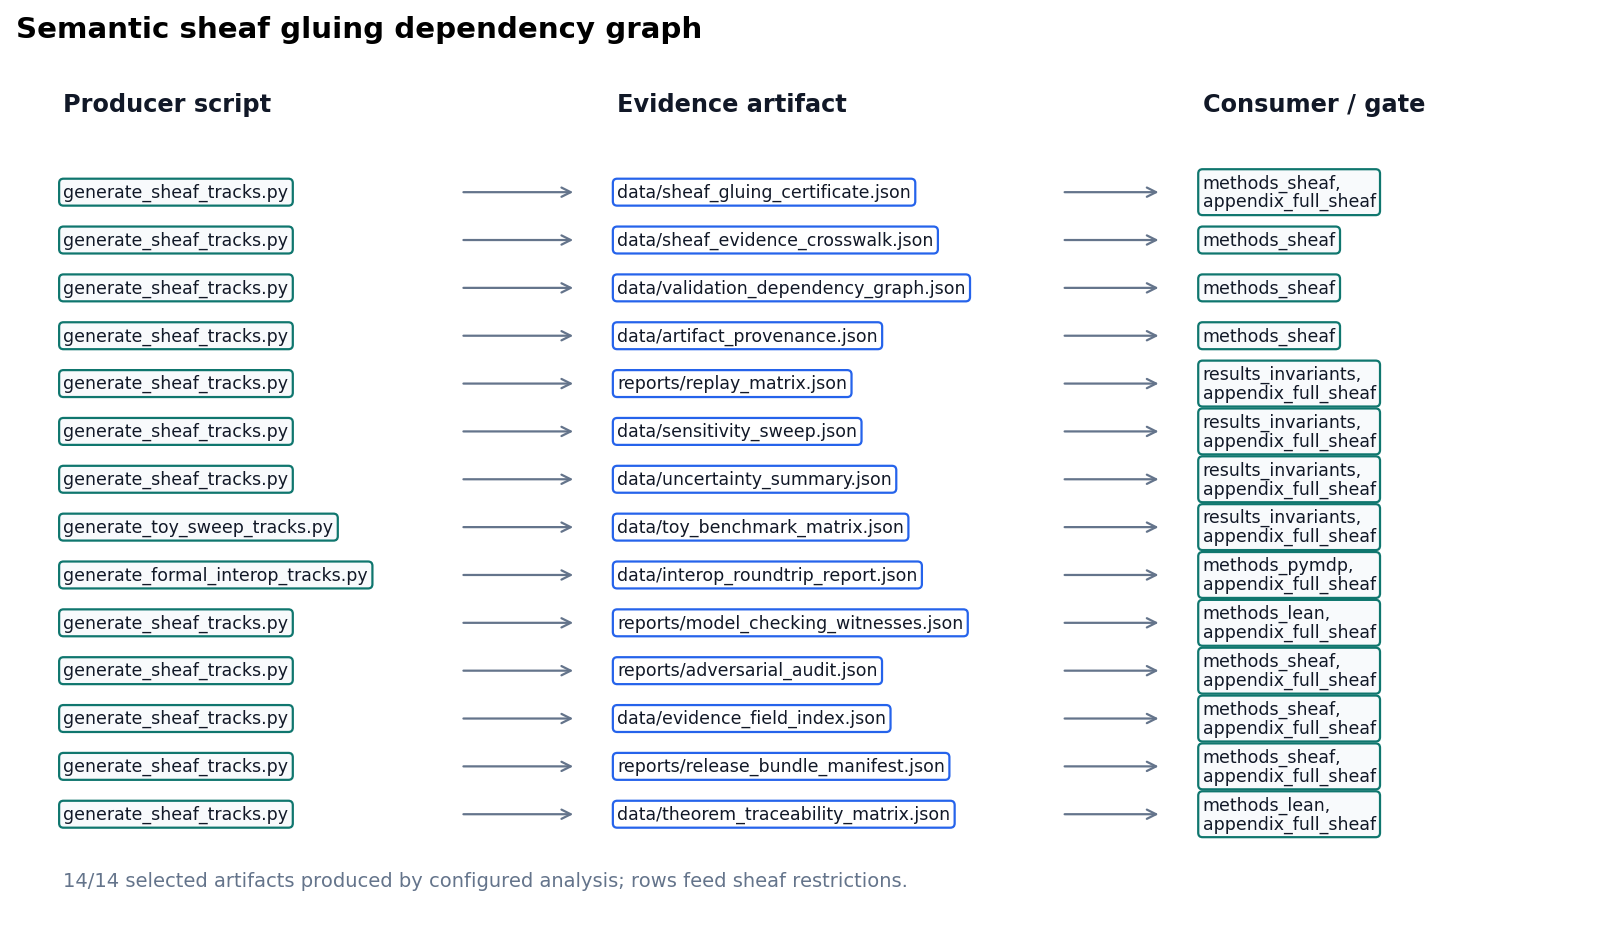
\includegraphics[width=0.95\linewidth,height=0.5\textheight,keepaspectratio,alt={Semantic gluing graph: configured producers, generated evidence artifacts, and validation consumers for the multi-track sheaf certificate.}]{../figures/semantic_gluing_graph.png}
\caption{Semantic gluing graph: configured producers, generated evidence
artifacts, and validation consumers for the multi-track sheaf
certificate.}\label{fig:semantic_gluing_graph}
\end{figure}

\begin{figure}
\centering
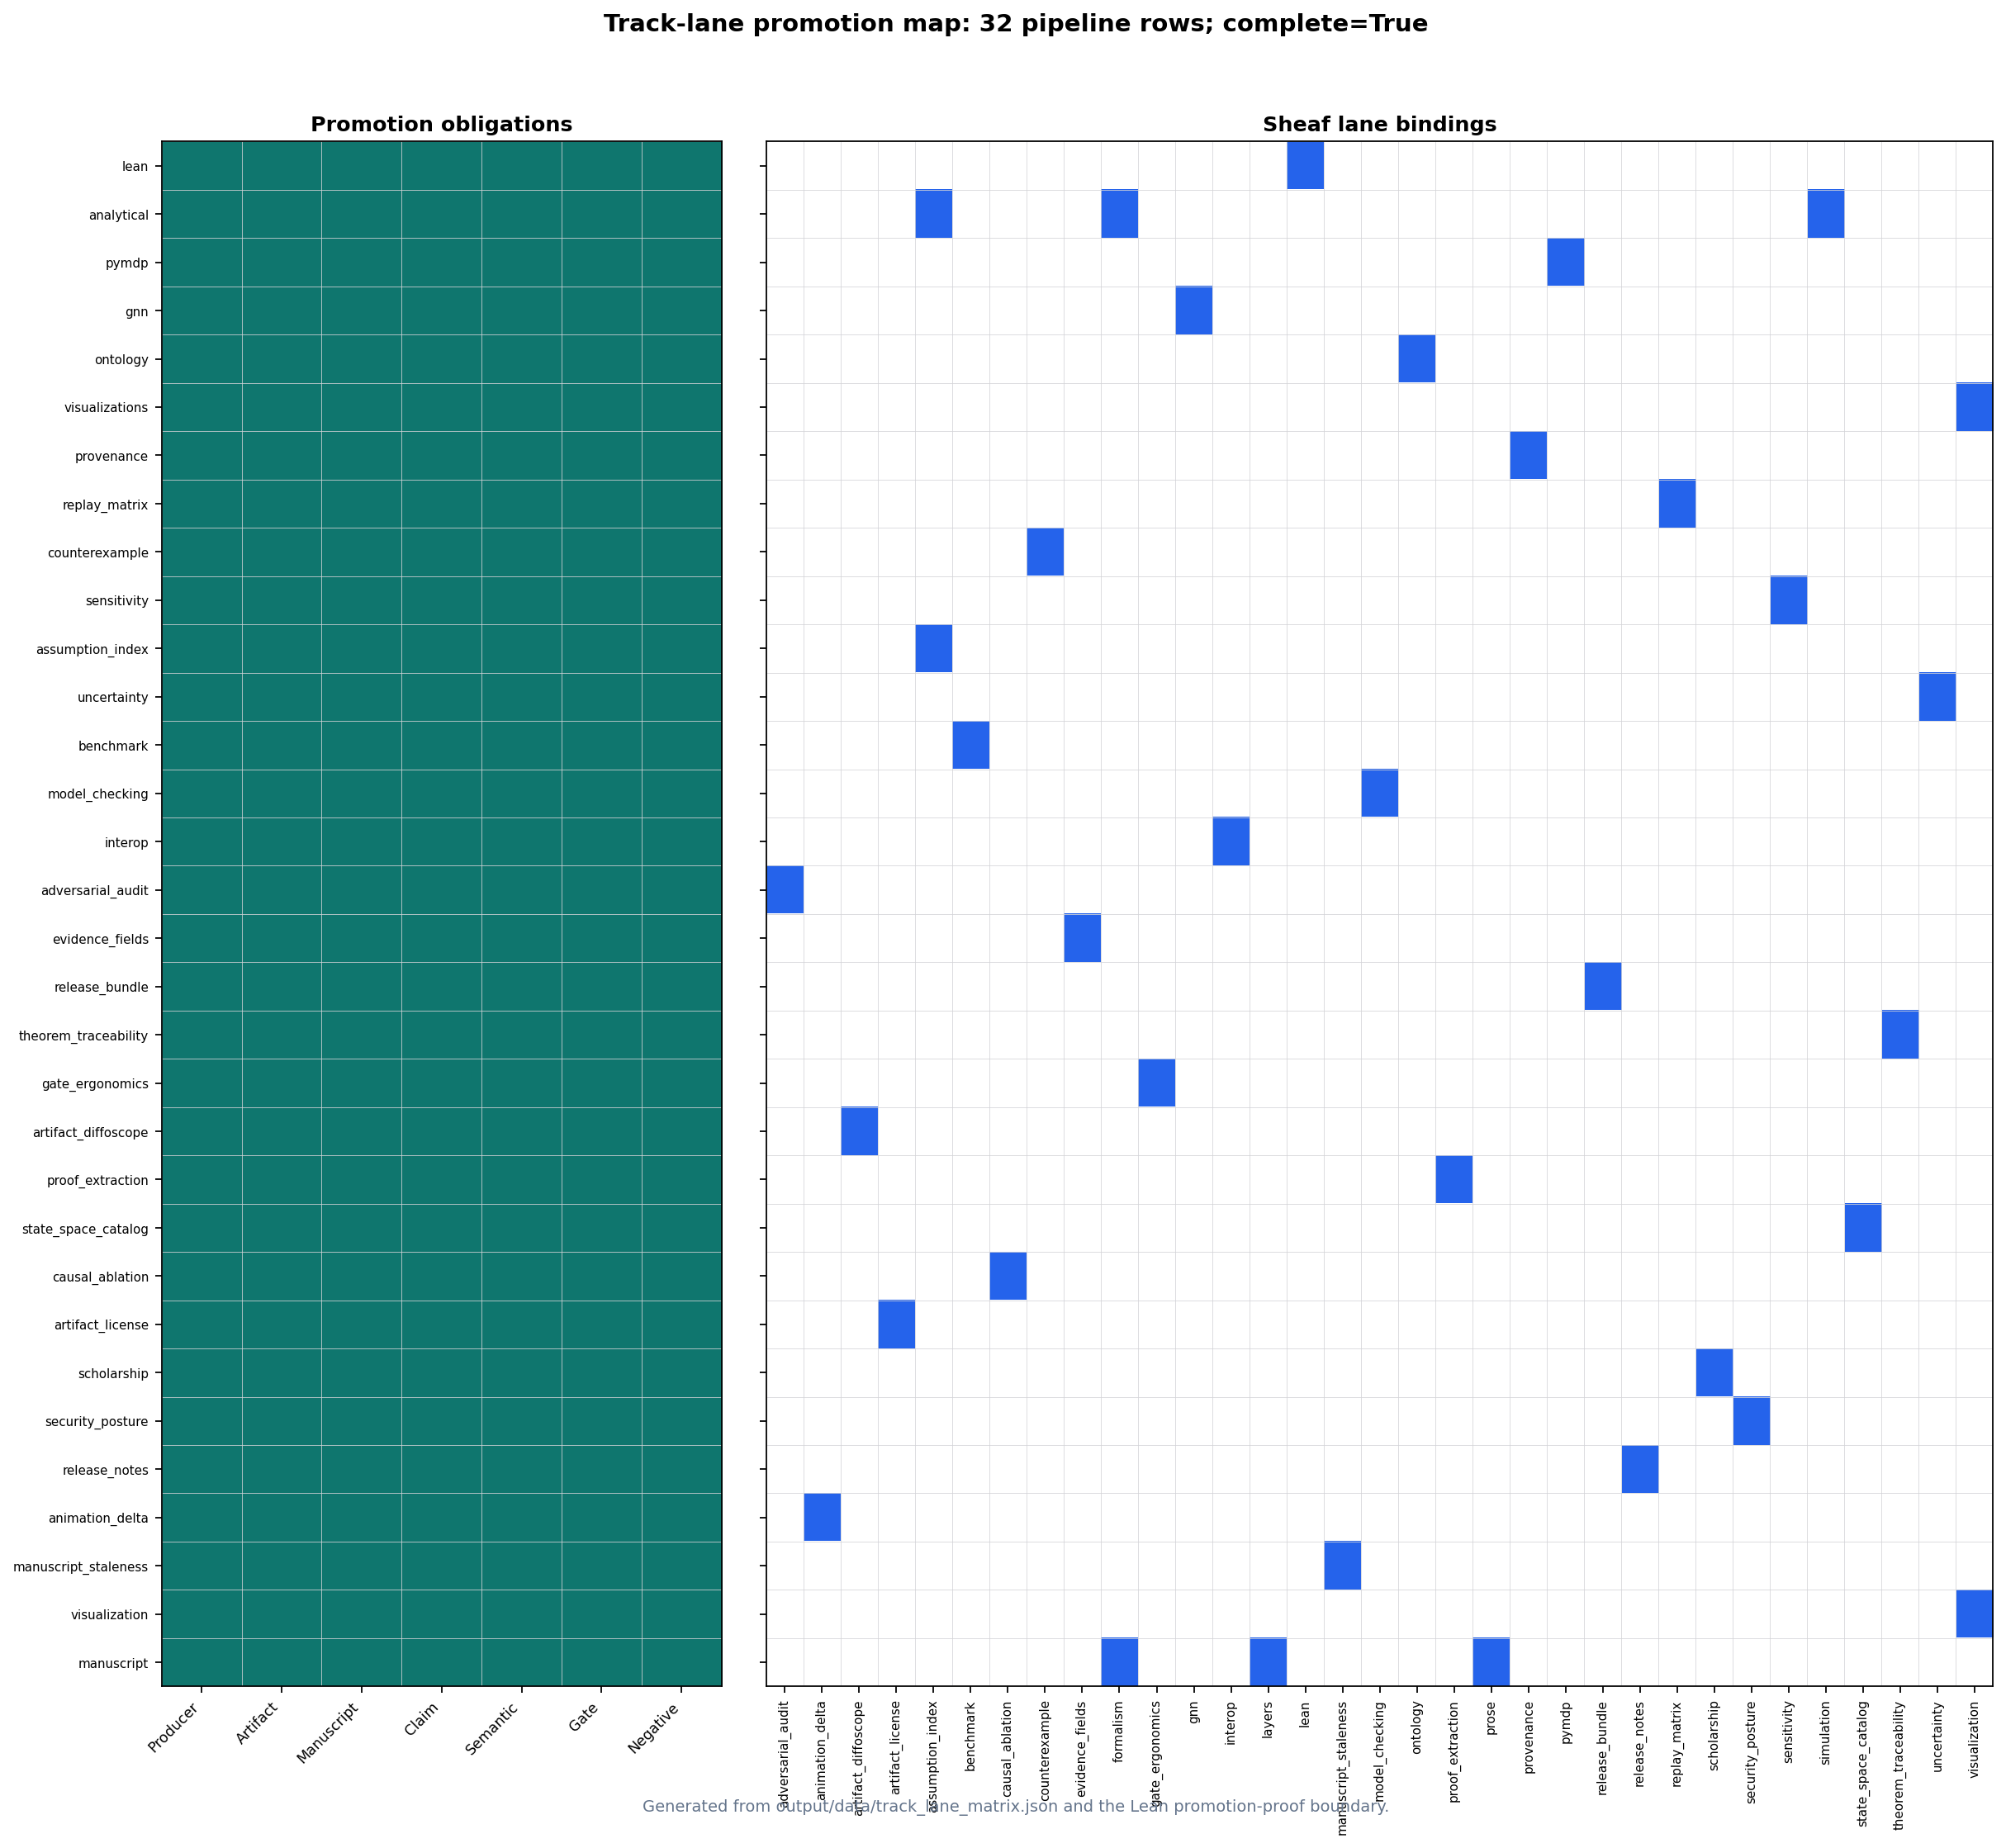
\includegraphics[width=0.98\linewidth,height=0.5\textheight,keepaspectratio,alt={Track-lane promotion map: 32 pipeline-to-sheaf rows with complete promotion status true. Left: seven promotion-rule obligations; right: sheaf fragment bindings.}]{../figures/track_lane_promotion_map.png}
\caption{Track-lane promotion map: 32 pipeline-to-sheaf rows with
complete promotion status true. Left: seven promotion-rule obligations;
right: sheaf fragment bindings.}\label{fig:track_lane_promotion_map}
\end{figure}

\begin{figure}
\centering
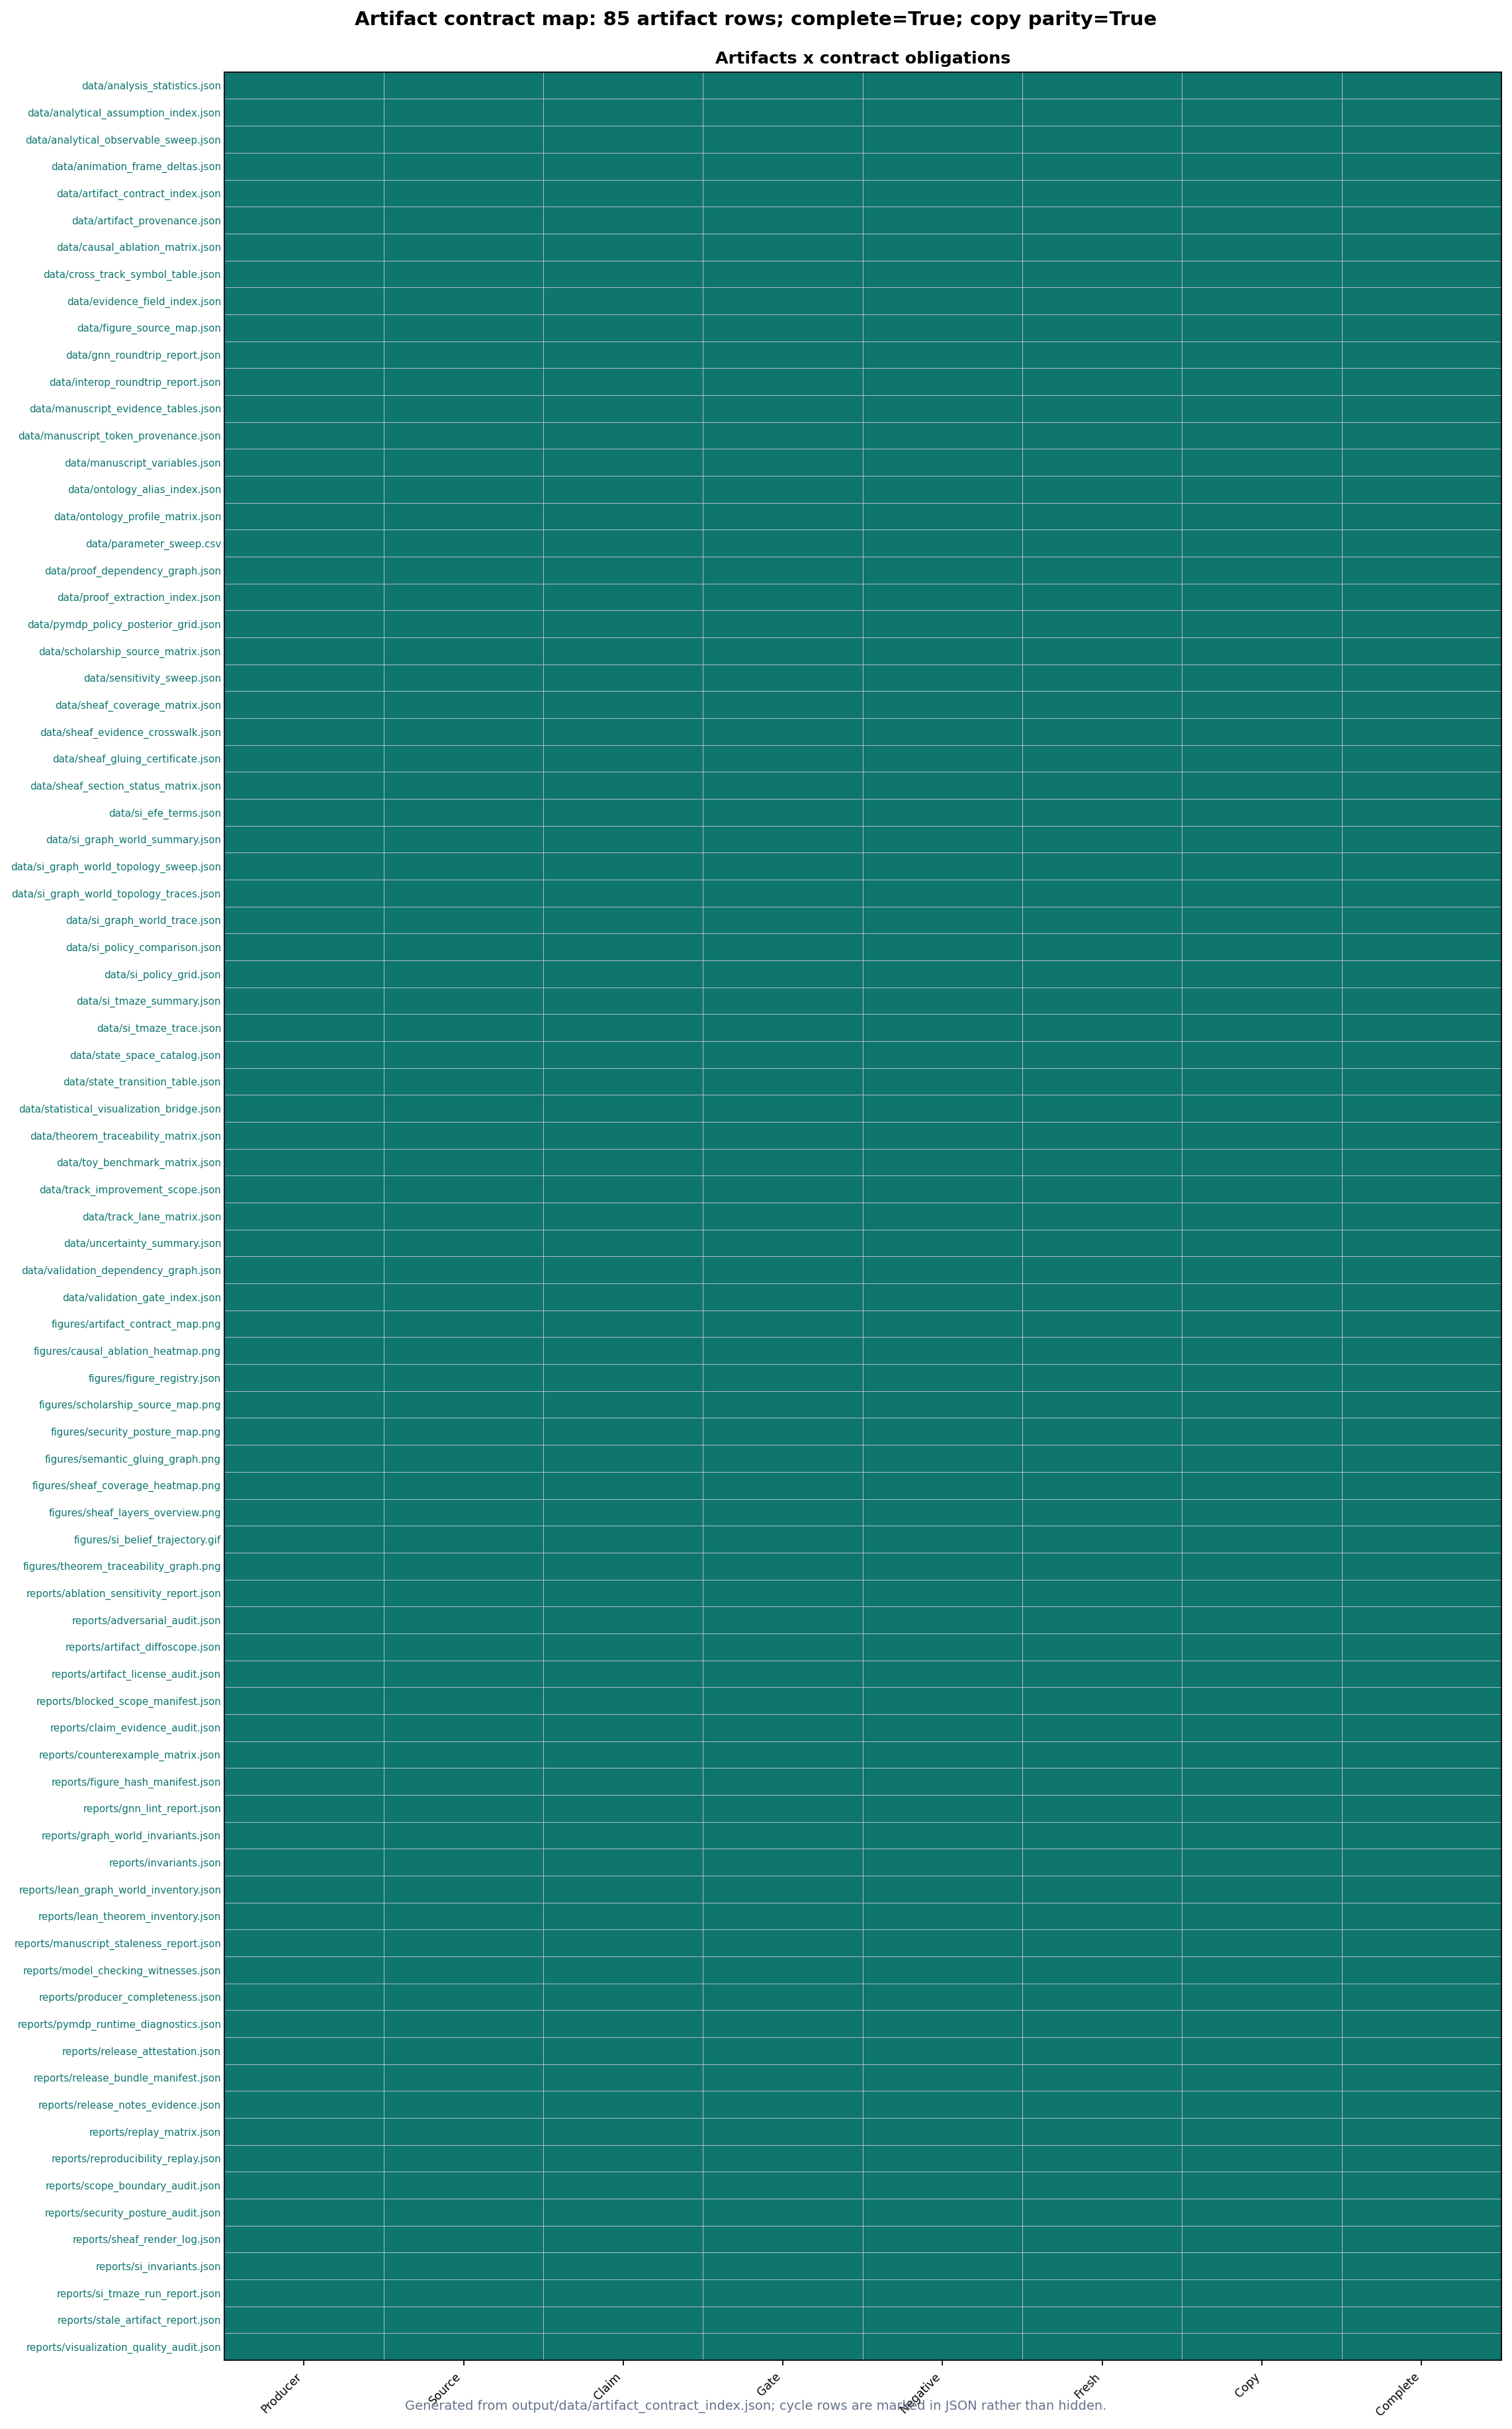
\includegraphics[width=0.98\linewidth,height=0.5\textheight,keepaspectratio,alt={Artifact contract map: 85 generated artifact rows with complete contract status true and copied-output parity complete true. Cycle rows are explicit in output/data/artifact\_contract\_index.json.}]{../figures/artifact_contract_map.png}
\caption{Artifact contract map: 85 generated artifact rows with complete
contract status true and copied-output parity complete true. Cycle rows
are explicit in
\protect\breaktt{output/data/artifact\_contract\_index.json}.}\label{fig:artifact_contract_map}
\end{figure}

\begin{figure}
\centering
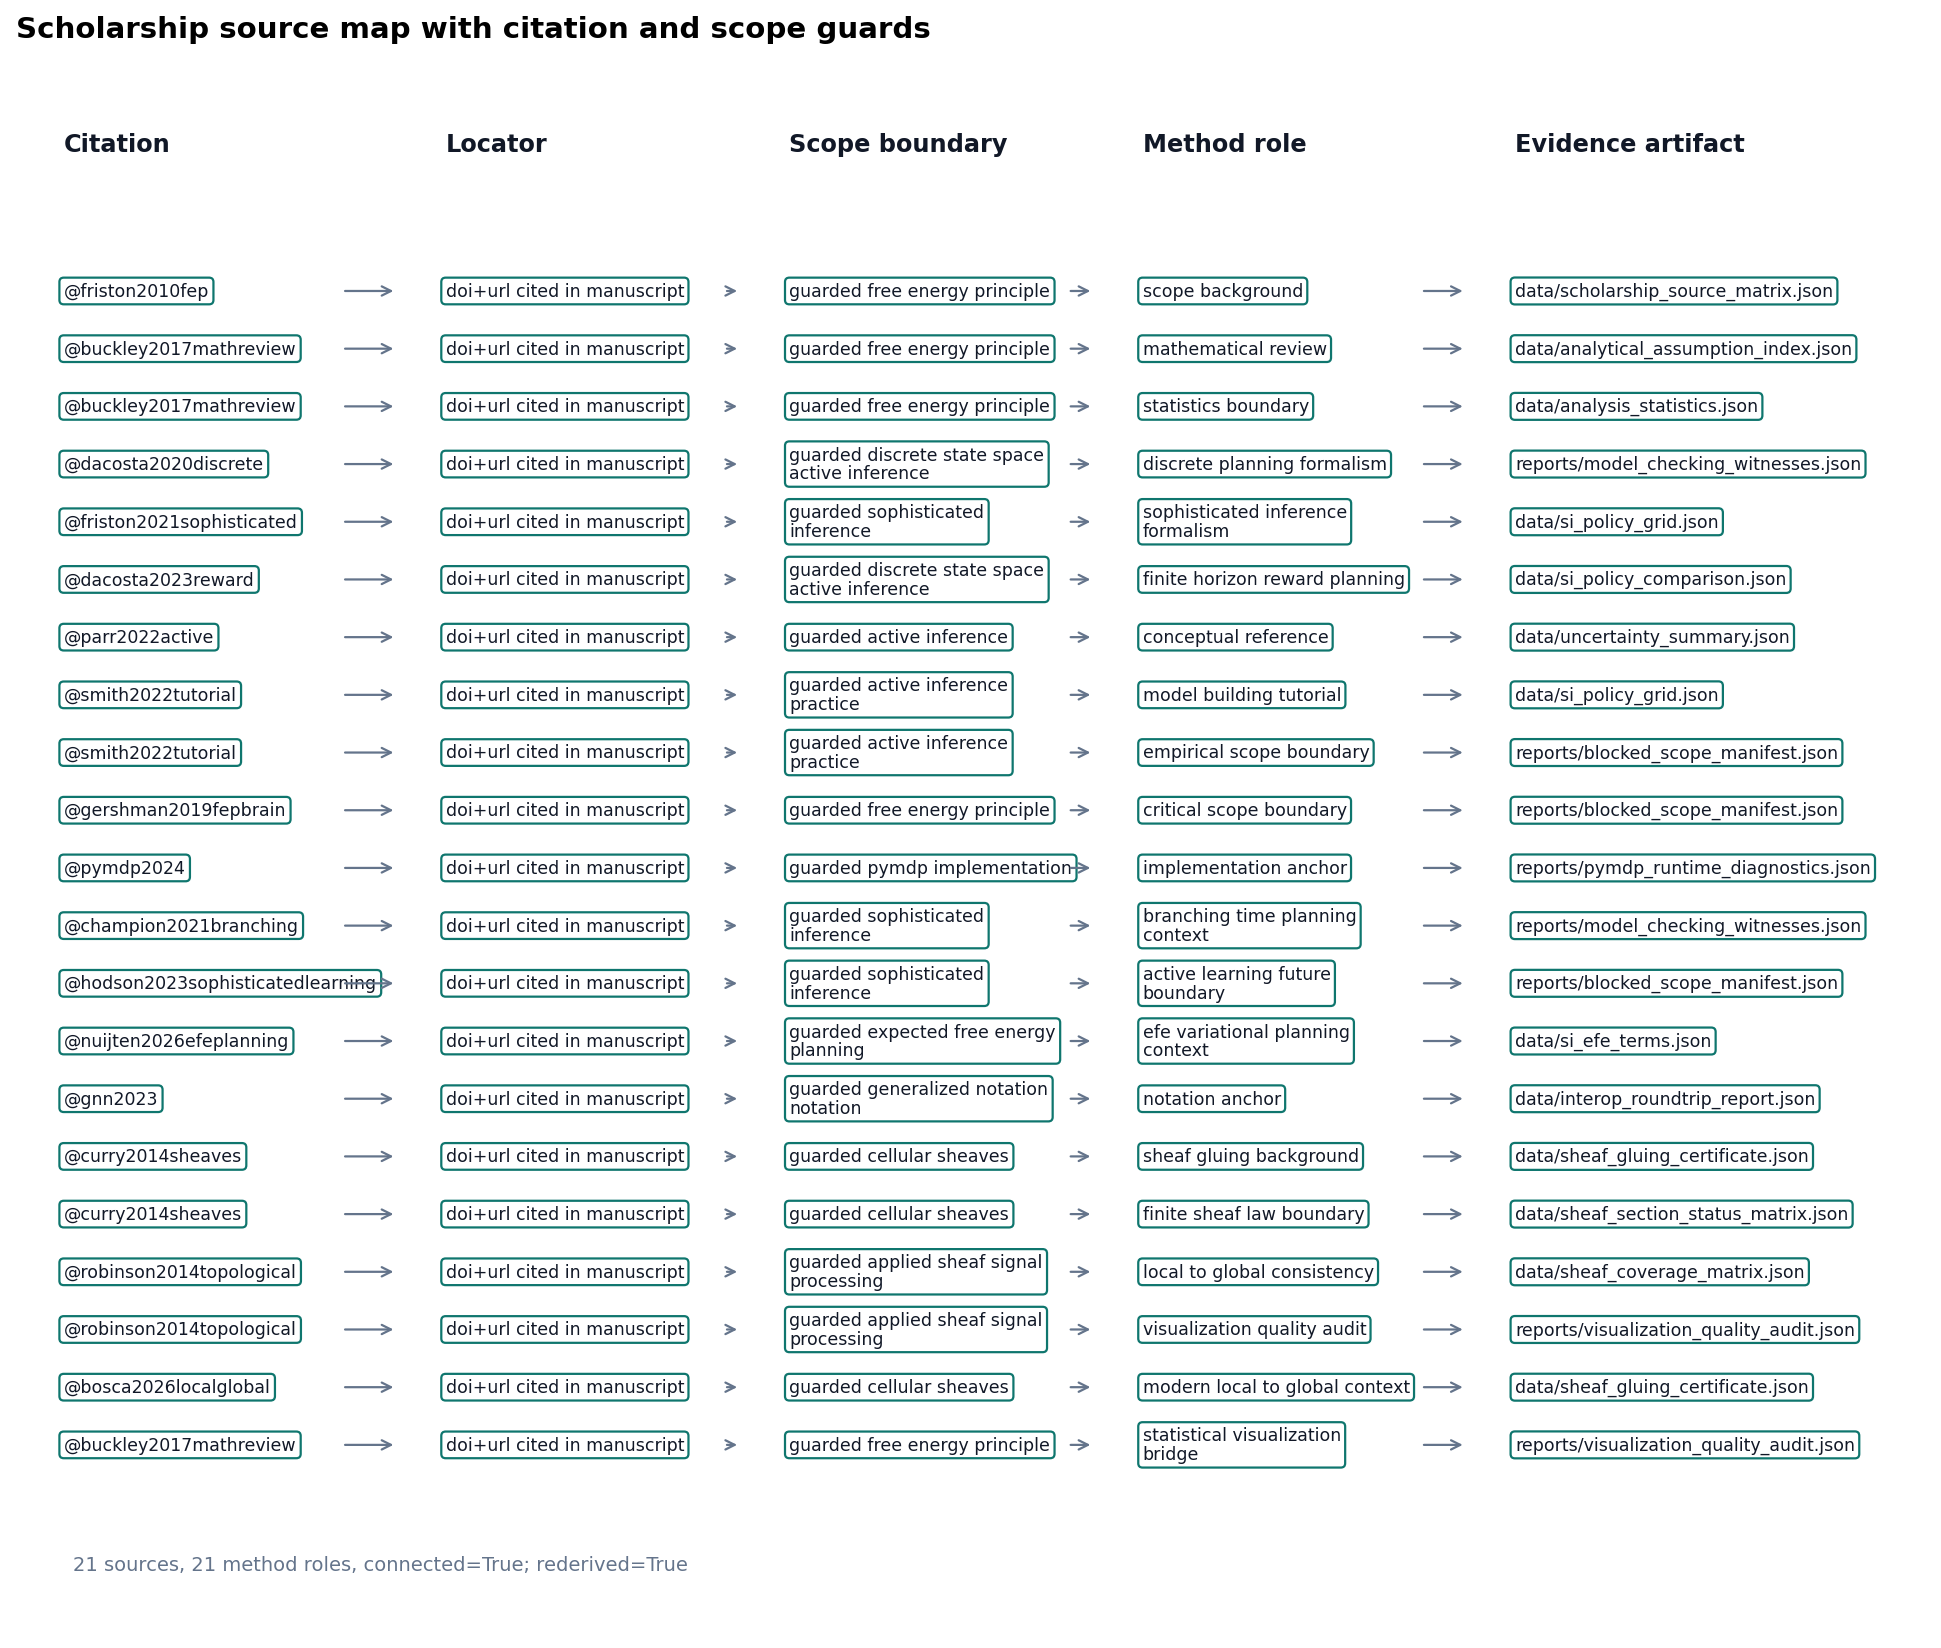
\includegraphics[width=0.95\linewidth,height=0.5\textheight,keepaspectratio,alt={Scholarship source map: 21 source rows across 21 method roles and 10 source families. Connected status: true; row evidence rederived: true.}]{../figures/scholarship_source_map.png}
\caption{Scholarship source map: 21 source rows across 21 method roles
and 10 source families. Connected status: true; row evidence rederived:
true.}\label{fig:scholarship_source_map}
\end{figure}

\begin{figure}
\centering
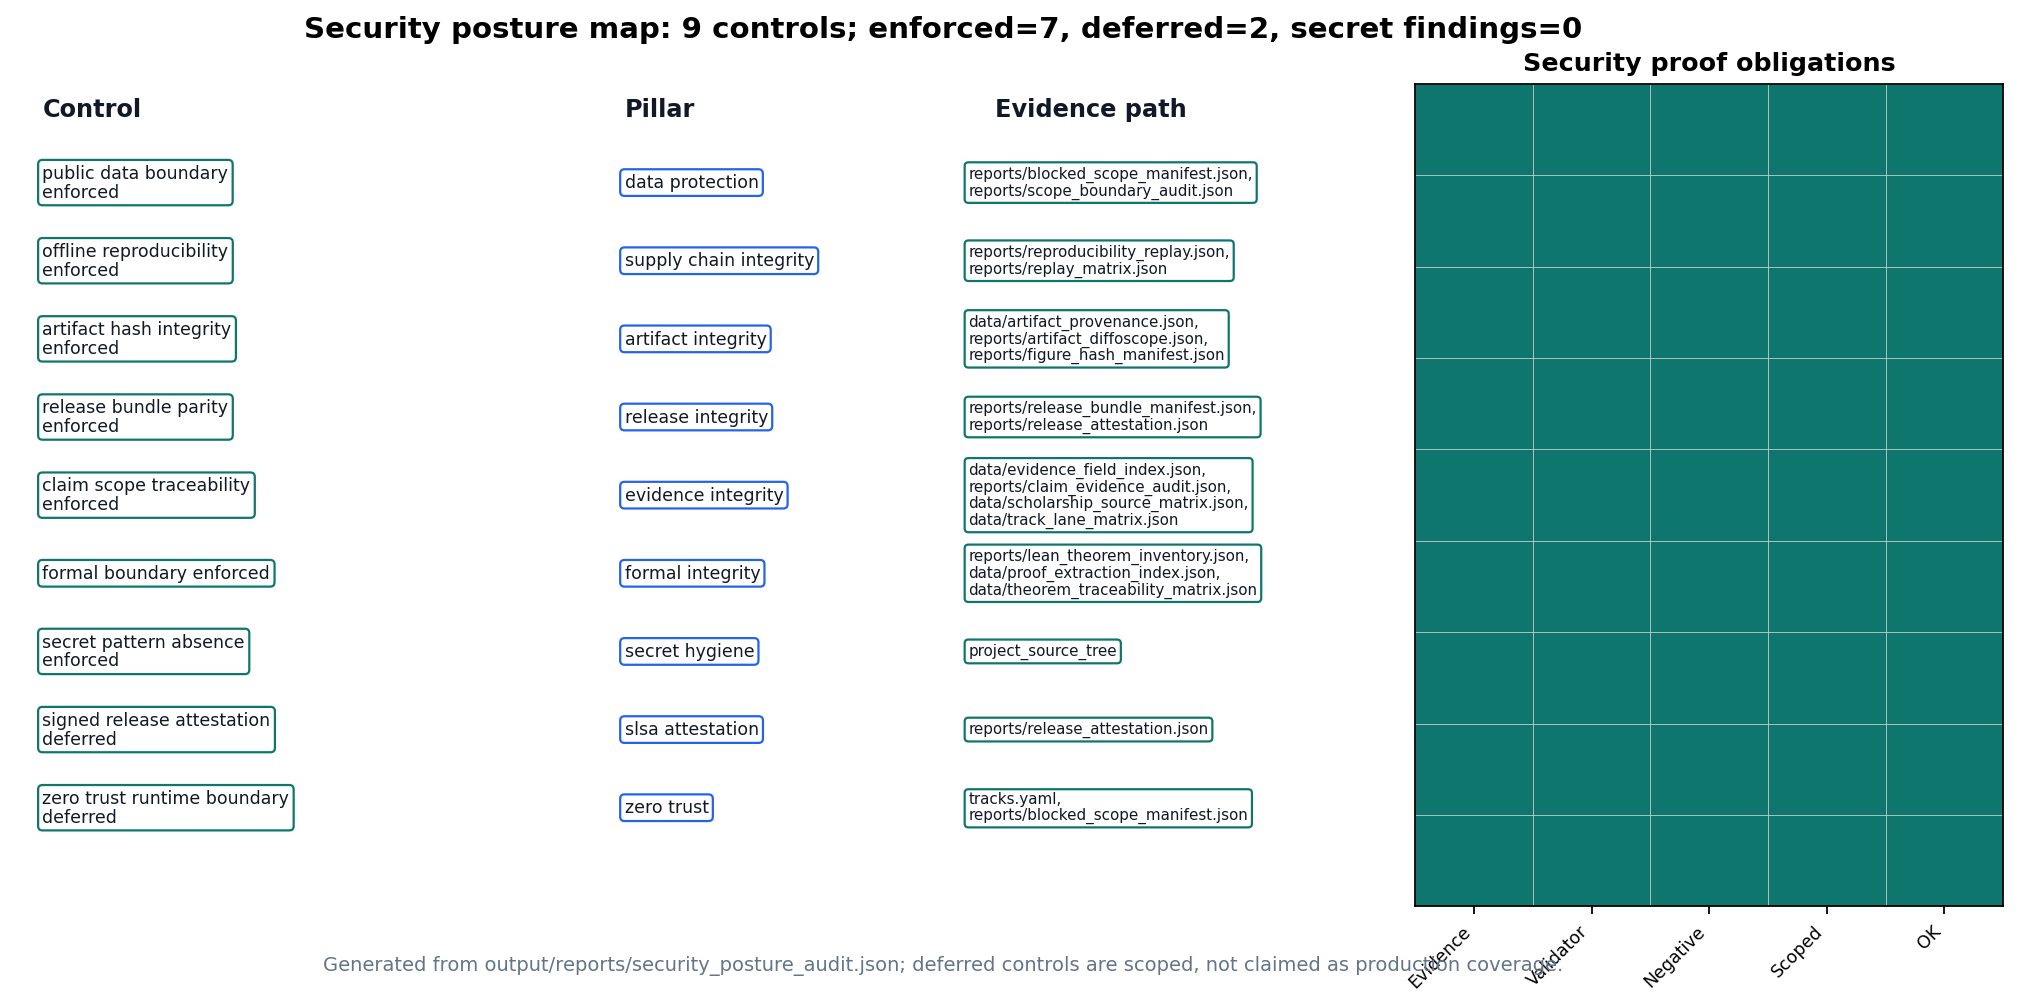
\includegraphics[width=0.96\linewidth,height=0.5\textheight,keepaspectratio,alt={Security posture map: 9 controls, 7 enforced and 2 scoped as deferred; secret findings: 0; high-risk gaps: 0.}]{../figures/security_posture_map.png}
\caption{Security posture map: 9 controls, 7 enforced and 2 scoped as
deferred; secret findings: 0; high-risk gaps:
0.}\label{fig:security_posture_map}
\end{figure}

The \texttt{provenance} fragment makes artifact lineage a live canonical
sheaf track. The configured producer \breaktt{generate\_sheaf\_tracks.py}
writes \breaktt{output/data/artifact\_provenance.json}, which hashes 85
required toy artifacts and records producer scripts, source commit,
deterministic seed fields, config digests, and 5 artifact bundles.
Publication claims that depend on generated files must be traceable to
this lineage table or to a narrower artifact-specific certificate.

The provenance claim is intentionally limited: every listed artifact
exists, has a SHA-256 digest or an explicit cycle exclusion, is produced
by a configured analysis script, and carries seed/config provenance
(\texttt{85} seeded rows; all seeded flag \texttt{true}; bundle-complete
flag \texttt{true}). A changed file, missing producer, or stale saved
digest is a validation failure, not a prose warning.

The \texttt{counterexample} fragment records expected-failure fixtures
as first-class evidence.
\breaktt{output/reports/counterexample\_matrix.json} lists 25 negative
controls that intentionally mutate ontology mappings, semantic
certificates, graph-world trace agreement, typed claim evidence, replay
rows, release parity, and provenance hashes.

The matrix is not an empirical result. It is a falsifiability ledger:
each row names the gate that must fail and the test that proves the
failure path remains live.

The \breaktt{adversarial\_audit} fragment makes expected failures part of
the sheaf rather than an informal test note.
\breaktt{output/reports/adversarial\_audit.json} records 25 known-bad
rows and 0 known-bad rows passing; publication proceeds only when every
row is documented as an expected failure and mapped to a gate.

The audit rows target the same failure modes as the semantic
certificate: incomplete sweep cells, unnormalized uncertainty rows,
interop field loss, stale certificate state, and empirical-scope
leakage. The scope boundary remains toy-only: \texttt{toy\_only\_pass}.

The \texttt{evidence\_fields} fragment indexes the exact artifact fields
that support typed claims and hydrated manuscript tokens.
\breaktt{output/data/evidence\_field\_index.json} records 97 field rows,
and the track passes only when every referenced JSONPath or dotted field
is present (\texttt{true}).

The \texttt{release\_bundle} fragment records whether the canonical
deliverables exist before copying and whether copied root outputs match
or are explicitly deferred until the copy stage.
\breaktt{output/reports/release\_bundle\_manifest.json} tracks 38
required deliverables with source-present flag \texttt{true}.

The bundle contract is now indexed artifact-by-artifact rather than
inferred from isolated reports.
\breaktt{output/data/artifact\_contract\_index.json} contains 85
generated artifact rows; each row binds its producer, configured script,
pipeline/sheaf lanes, manuscript consumers, claim predicates,
validators, negative control, freshness status, and copied-output
parity. The aggregate row-complete flag is \texttt{true}, and
copied-root parity completeness is \texttt{true}.

The \texttt{gate\_ergonomics} fragment turns validation commands into
evidence rows. \breaktt{output/data/validation\_gate\_index.json} records
26 gate rows, each naming required inputs and the negative-control
surface that should fail closed.

\breaktt{output/data/track\_lane\_matrix.json} is the cross-track audit
table for the same gate surface: 32 pipeline rows map to sheaf
fragments, producer scripts, primary artifacts, validation gates, and
manuscript consumers, with completion flag \texttt{true}.

\subsubsection{Artifact diffoscope
track}\label{artifact-diffoscope-track}

The \breaktt{artifact\_diffoscope} track compares saved provenance hashes
against live artifact hashes at the artifact root JSONPath. Its proof
artifact is \breaktt{output/reports/artifact\_diffoscope.json}: it
currently records 41 comparison rows, with equality status
\texttt{true}.

\subsubsection{Artifact license track}\label{artifact-license-track}

The \breaktt{artifact\_license} track classifies generated and
project-source artifacts under the public project license boundary. Its
audit artifact is \breaktt{output/reports/artifact\_license\_audit.json}:
it currently records 85 rows, with license-safe status \texttt{true}.

The \texttt{scholarship} fragment turns citations into an audited method
surface rather than decorative bibliography.
\breaktt{output/data/scholarship\_source\_matrix.json} records 21 source
rows across 21 method roles and 10 source families, including 3
quantitative/statistical or visualization-quality method roles;
fig.~\ref{fig:scholarship_source_map} renders the resulting
source-to-artifact map with 1 locator kinds. The row set connects
foundational free-energy and active-inference references
\citep{friston2010fep, buckley2017mathreview, dacosta2020discrete, parr2022active, smith2022tutorial},
planning context \citep{champion2021branching, nuijten2026efeplanning},
implementation and notation anchors \citep{pymdp2024, gnn2023}, and
applied sheaf/local-to-global sources
\citep{curry2014sheaves, robinson2014topological, bosca2026localglobal}
to the exact artifact or method role they support.

The validation claim is deliberately narrow: every row must have a
bibliography entry with a DOI or URL, a manuscript citation, registered
sheaf tracks, bound manifest consumer sections, an existing evidence
artifact, and a scope-guarded claim-boundary statement. The saved matrix
is then rederived from live bibliography, manuscript, registry,
manifest, and artifact evidence before validation accepts it
(\texttt{true}), so a forged row-level boolean cannot launder a
disconnected source. The added statistics and visualization rows point
to \breaktt{analysis\_statistics.json} and
\breaktt{visualization\_quality\_audit.json}, including a
statistical-visualization bridge row, so the scholarship track now
distinguishes method lineage from the generated numerical,
figure-quality, and figure-provenance evidence. The hydrated flags
\texttt{true}, \texttt{true}, and \texttt{true} are therefore
source-traceability and scope-control claims, not claims that the toy
results inherit empirical support from the cited literature.

The newer arXiv rows are intentionally constrained. They situate the toy
EFE and planning artifacts against branching-time and
variational-planning work, and they situate the finite manuscript sheaf
against modern local-to-global computation framing, but none of those
citations promotes empirical, neural network, or scalable-agent
performance claims for this exemplar.

The security-posture track treats the public exemplar itself as the
defended asset. \breaktt{output/reports/security\_posture\_audit.json}
records 9 controls: 7 enforced local controls and 2 production-security
obligations that are explicitly deferred rather than claimed. The
enforced rows cover public-data boundaries, offline reproducibility,
artifact hashes, copied-output parity, claim/scope traceability, the
Lean boundary, and a source/config secret-pattern scan.

The audit is intentionally not a production certification. It records 0
high-risk local gaps and 0 high-risk secret-pattern findings; the
all-controls flag is \texttt{true}, and all listed evidence is present:
\texttt{true}. Deferred rows cover signed provenance/SBOM release
attestation and zero-trust runtime controls, which require
deployment-specific identity, device posture, logging, and signing
infrastructure outside this toy-only manuscript.

The \breaktt{manuscript\_staleness} fragment closes the hydration loop.
\breaktt{output/reports/manuscript\_staleness\_report.json} checks 322
manuscript token bindings against the current generated variables after
resolved markdown is written; the pass flag is \texttt{true}.

This is a publication-systems claim, not a domain result. A stale
hydrated value, unresolved token, or missing resolved section becomes a
validation failure before PDF or web outputs are accepted.

\subsection{Sheaf fragment track
registry}\label{sheaf-fragment-track-registry}

Compose order and renderer bindings from
\breaktt{manuscript/sheaf/tracks.yaml}.

{\def\LTcaptype{none} % do not increment counter
\begin{longtable}[]{@{}
  >{\raggedleft\arraybackslash}p{(\linewidth - 12\tabcolsep) * \real{0.1818}}
  >{\raggedright\arraybackslash}p{(\linewidth - 12\tabcolsep) * \real{0.1364}}
  >{\raggedright\arraybackslash}p{(\linewidth - 12\tabcolsep) * \real{0.1364}}
  >{\raggedright\arraybackslash}p{(\linewidth - 12\tabcolsep) * \real{0.1364}}
  >{\raggedright\arraybackslash}p{(\linewidth - 12\tabcolsep) * \real{0.1364}}
  >{\raggedright\arraybackslash}p{(\linewidth - 12\tabcolsep) * \real{0.1364}}
  >{\raggedright\arraybackslash}p{(\linewidth - 12\tabcolsep) * \real{0.1364}}@{}}
\toprule\noalign{}
\begin{minipage}[b]{\linewidth}\raggedleft
Order
\end{minipage} & \begin{minipage}[b]{\linewidth}\raggedright
Track id
\end{minipage} & \begin{minipage}[b]{\linewidth}\raggedright
Label
\end{minipage} & \begin{minipage}[b]{\linewidth}\raggedright
Renderer
\end{minipage} & \begin{minipage}[b]{\linewidth}\raggedright
Paper role
\end{minipage} & \begin{minipage}[b]{\linewidth}\raggedright
Paper use
\end{minipage} & \begin{minipage}[b]{\linewidth}\raggedright
Optional
\end{minipage} \\
\midrule\noalign{}
\endhead
\bottomrule\noalign{}
\endlastfoot
10 & \texttt{prose} & Narrative prose & \texttt{markdown} & Narrative
framing and argument flow & Supports the narrative spine for each
composed paper section. & No \\
20 & \texttt{formalism} & Mathematical formalism & \texttt{markdown} &
Mathematical definitions and equations & States the finite equations,
laws, and boundary assumptions used by prose claims. & No \\
30 & \texttt{simulation} & Analytical simulation notes &
\texttt{markdown} & Deterministic toy analysis evidence & Connects
analytical sweeps and toy simulations to results claims. & No \\
32 & \breaktt{assumption\_index} & Analytical assumption index &
\texttt{markdown} & Assumption boundary ledger & Lists finite-model
assumptions so analytical claims stay scoped. & No \\
35 & \texttt{layers} & Sheaf layers tables & \texttt{layers\_report} &
Registry and binding disclosure & Generates the track registry, binding
matrix, and evidence crosswalk tables. & Yes \\
40 & \texttt{pymdp} & pymdp harness artifacts & \texttt{markdown} &
Active-inference implementation evidence & Binds pymdp traces, runtime
diagnostics, and policy comparisons to methods and results. & No \\
41 & \texttt{interop} & GNN/ontology/JSON interop checks &
\texttt{markdown} & Cross-format compatibility evidence & Shows that
GNN, ontology, and JSON artifacts preserve model meaning. & No \\
42 & \texttt{provenance} & Artifact provenance and bundle lineage spine
& \texttt{markdown} & Artifact lineage evidence & Documents producers,
hashes, seeds, and bundle lineage for generated claims. & No \\
45 & \texttt{replay\_matrix} & Deterministic replay matrix &
\texttt{markdown} & Reproducibility replay evidence & Shows configured
producers replay and match their expected artifacts. & No \\
48 & \texttt{counterexample} & Expected-failure counterexamples &
\texttt{markdown} & Falsifiability negative controls & Records known-bad
fixtures that must fail validation gates. & No \\
50 & \breaktt{adversarial\_audit} & Adversarial audit matrix &
\texttt{markdown} & Adversarial robustness evidence & Documents stress
cases and expected failures for sheaf-track claims. & No \\
52 & \texttt{evidence\_fields} & Evidence field index &
\texttt{markdown} & Claim field traceability & Maps evidence fields to
sections and artifacts for claim hydration. & No \\
53 & \texttt{release\_bundle} & Release bundle parity manifest &
\texttt{markdown} & Release artifact parity evidence & Checks that
required deliverables exist and copied outputs match or defer
explicitly. & No \\
54 & \texttt{gate\_ergonomics} & Validation gate ergonomics &
\texttt{markdown} & Validation workflow index & Explains the gates a
reader or maintainer can rerun locally. & No \\
55 & \breaktt{artifact\_diffoscope} & Artifact diffoscope &
\texttt{markdown} & Artifact equality evidence & Compares generated and
copied artifacts to surface publication drift. & No \\
56 & \breaktt{artifact\_license} & Artifact license audit &
\texttt{markdown} & License safety evidence & Records license status for
artifacts included in release surfaces. & No \\
57 & \texttt{scholarship} & Source-backed scholarship matrix &
\texttt{markdown} & Scholarship and method-source lineage & Connects
cited sources to method roles, sections, and generated evidence. & No \\
58 & \breaktt{security\_posture} & Security posture audit &
\texttt{markdown} & Public release security boundary evidence &
Separates enforced local controls from deferred production-security
obligations. & No \\
60 & \texttt{sensitivity} & Toy sensitivity sweep & \texttt{markdown} &
Parameter sensitivity evidence & Summarizes deterministic toy
perturbations behind robustness claims. & No \\
62 & \texttt{uncertainty} & Toy uncertainty summaries &
\texttt{markdown} & Uncertainty summary evidence & Reports normalized
uncertainty bins and summaries for finite toy analyses. & No \\
65 & \texttt{benchmark} & Compact toy benchmark matrix &
\texttt{markdown} & Toy benchmark comparison evidence & Shows compact
model comparisons used to bound toy-only claims. & No \\
66 & \breaktt{manuscript\_staleness} & Hydrated manuscript staleness
report & \texttt{markdown} & Manuscript freshness evidence & Checks
hydrated sections against current generated artifacts and variables. &
No \\
67 & \texttt{visualization} & Figure references &
\texttt{section\_figures} & Figure evidence and communication & Injects
registry figures into section-specific evidence blocks. & No \\
70 & \texttt{lean} & Lean boundary fragment & \texttt{markdown} & Formal
proof boundary evidence & Separates proved Lean witnesses from
intentionally scoped formal boundaries. & No \\
75 & \texttt{model\_checking} & Finite-state model checking witnesses &
\texttt{markdown} & Exhaustive finite-model evidence & Lists
model-checking witnesses for finite state-space claims. & No \\
76 & \breaktt{theorem\_traceability} & Lean theorem traceability matrix &
\texttt{markdown} & Theorem dependency traceability & Links theorem rows
to proof dependencies and finite model witnesses. & No \\
77 & \breaktt{proof\_extraction} & Lean proof extraction index &
\texttt{markdown} & Constructive proof extraction evidence & Shows
extracted theorem artifacts remain constructive and available. & No \\
78 & \breaktt{state\_space\_catalog} & Finite state-space catalog &
\texttt{markdown} & Finite model catalog evidence & Enumerates reachable
states so toy models remain explicitly finite. & No \\
79 & \texttt{causal\_ablation} & Deterministic causal ablation matrix &
\texttt{markdown} & Causal ablation evidence & Summarizes deterministic
perturbation effects across toy topologies. & No \\
80 & \texttt{gnn} & GNN notation fragment & \texttt{markdown} & GNN
notation evidence & Documents notation and round-trip status for the
analytical model. & No \\
90 & \texttt{ontology} & Active Inference Ontology bindings &
\texttt{ontology\_yaml} & Ontology binding evidence & Maps local
variables to ontology terms for semantic consistency. & No \\
100 & \texttt{animation} & Animation fragment & \texttt{markdown} &
Dynamic trace visualization & Provides a deterministic GIF trace as
optional appendix evidence. & Yes \\
102 & \texttt{animation\_delta} & Animation frame-delta manifest &
\texttt{markdown} & Animation integrity evidence & Confirms animation
frames change and support the visual trace. & No \\
110 & \texttt{release\_notes} & Release notes evidence &
\texttt{markdown} & Release narrative evidence & Binds release-note
statements to source-backed artifacts. & No \\
\end{longtable}
}

\textbf{Track count:} 34 registered fragment types.

\subsection{IMRAD binding matrix}\label{imrad-binding-matrix}

Section rows versus fragment track columns. \textbf{P} = present (bound
and file exists); \textbf{---} = absent (not bound); \textbf{M} =
missing (bound, file absent).

{\def\LTcaptype{none} % do not increment counter
\begin{longtable}[]{@{}
  >{\raggedright\arraybackslash}p{(\linewidth - 68\tabcolsep) * \real{0.0286}}
  >{\raggedright\arraybackslash}p{(\linewidth - 68\tabcolsep) * \real{0.0286}}
  >{\raggedright\arraybackslash}p{(\linewidth - 68\tabcolsep) * \real{0.0286}}
  >{\raggedright\arraybackslash}p{(\linewidth - 68\tabcolsep) * \real{0.0286}}
  >{\raggedright\arraybackslash}p{(\linewidth - 68\tabcolsep) * \real{0.0286}}
  >{\raggedright\arraybackslash}p{(\linewidth - 68\tabcolsep) * \real{0.0286}}
  >{\raggedright\arraybackslash}p{(\linewidth - 68\tabcolsep) * \real{0.0286}}
  >{\raggedright\arraybackslash}p{(\linewidth - 68\tabcolsep) * \real{0.0286}}
  >{\raggedright\arraybackslash}p{(\linewidth - 68\tabcolsep) * \real{0.0286}}
  >{\raggedright\arraybackslash}p{(\linewidth - 68\tabcolsep) * \real{0.0286}}
  >{\raggedright\arraybackslash}p{(\linewidth - 68\tabcolsep) * \real{0.0286}}
  >{\raggedright\arraybackslash}p{(\linewidth - 68\tabcolsep) * \real{0.0286}}
  >{\raggedright\arraybackslash}p{(\linewidth - 68\tabcolsep) * \real{0.0286}}
  >{\raggedright\arraybackslash}p{(\linewidth - 68\tabcolsep) * \real{0.0286}}
  >{\raggedright\arraybackslash}p{(\linewidth - 68\tabcolsep) * \real{0.0286}}
  >{\raggedright\arraybackslash}p{(\linewidth - 68\tabcolsep) * \real{0.0286}}
  >{\raggedright\arraybackslash}p{(\linewidth - 68\tabcolsep) * \real{0.0286}}
  >{\raggedright\arraybackslash}p{(\linewidth - 68\tabcolsep) * \real{0.0286}}
  >{\raggedright\arraybackslash}p{(\linewidth - 68\tabcolsep) * \real{0.0286}}
  >{\raggedright\arraybackslash}p{(\linewidth - 68\tabcolsep) * \real{0.0286}}
  >{\raggedright\arraybackslash}p{(\linewidth - 68\tabcolsep) * \real{0.0286}}
  >{\raggedright\arraybackslash}p{(\linewidth - 68\tabcolsep) * \real{0.0286}}
  >{\raggedright\arraybackslash}p{(\linewidth - 68\tabcolsep) * \real{0.0286}}
  >{\raggedright\arraybackslash}p{(\linewidth - 68\tabcolsep) * \real{0.0286}}
  >{\raggedright\arraybackslash}p{(\linewidth - 68\tabcolsep) * \real{0.0286}}
  >{\raggedright\arraybackslash}p{(\linewidth - 68\tabcolsep) * \real{0.0286}}
  >{\raggedright\arraybackslash}p{(\linewidth - 68\tabcolsep) * \real{0.0286}}
  >{\raggedright\arraybackslash}p{(\linewidth - 68\tabcolsep) * \real{0.0286}}
  >{\raggedright\arraybackslash}p{(\linewidth - 68\tabcolsep) * \real{0.0286}}
  >{\raggedright\arraybackslash}p{(\linewidth - 68\tabcolsep) * \real{0.0286}}
  >{\raggedright\arraybackslash}p{(\linewidth - 68\tabcolsep) * \real{0.0286}}
  >{\raggedright\arraybackslash}p{(\linewidth - 68\tabcolsep) * \real{0.0286}}
  >{\raggedright\arraybackslash}p{(\linewidth - 68\tabcolsep) * \real{0.0286}}
  >{\raggedright\arraybackslash}p{(\linewidth - 68\tabcolsep) * \real{0.0286}}
  >{\raggedright\arraybackslash}p{(\linewidth - 68\tabcolsep) * \real{0.0286}}@{}}
\toprule\noalign{}
\begin{minipage}[b]{\linewidth}\raggedright
Section
\end{minipage} & \begin{minipage}[b]{\linewidth}\raggedright
prose
\end{minipage} & \begin{minipage}[b]{\linewidth}\raggedright
formalism
\end{minipage} & \begin{minipage}[b]{\linewidth}\raggedright
simulation
\end{minipage} & \begin{minipage}[b]{\linewidth}\raggedright
assumption\_index
\end{minipage} & \begin{minipage}[b]{\linewidth}\raggedright
layers
\end{minipage} & \begin{minipage}[b]{\linewidth}\raggedright
pymdp
\end{minipage} & \begin{minipage}[b]{\linewidth}\raggedright
interop
\end{minipage} & \begin{minipage}[b]{\linewidth}\raggedright
provenance
\end{minipage} & \begin{minipage}[b]{\linewidth}\raggedright
replay\_matrix
\end{minipage} & \begin{minipage}[b]{\linewidth}\raggedright
counterexample
\end{minipage} & \begin{minipage}[b]{\linewidth}\raggedright
adversarial\_audit
\end{minipage} & \begin{minipage}[b]{\linewidth}\raggedright
evidence\_fields
\end{minipage} & \begin{minipage}[b]{\linewidth}\raggedright
release\_bundle
\end{minipage} & \begin{minipage}[b]{\linewidth}\raggedright
gate\_ergonomics
\end{minipage} & \begin{minipage}[b]{\linewidth}\raggedright
artifact\_diffoscope
\end{minipage} & \begin{minipage}[b]{\linewidth}\raggedright
artifact\_license
\end{minipage} & \begin{minipage}[b]{\linewidth}\raggedright
scholarship
\end{minipage} & \begin{minipage}[b]{\linewidth}\raggedright
security\_posture
\end{minipage} & \begin{minipage}[b]{\linewidth}\raggedright
sensitivity
\end{minipage} & \begin{minipage}[b]{\linewidth}\raggedright
uncertainty
\end{minipage} & \begin{minipage}[b]{\linewidth}\raggedright
benchmark
\end{minipage} & \begin{minipage}[b]{\linewidth}\raggedright
manuscript\_staleness
\end{minipage} & \begin{minipage}[b]{\linewidth}\raggedright
visualization
\end{minipage} & \begin{minipage}[b]{\linewidth}\raggedright
lean
\end{minipage} & \begin{minipage}[b]{\linewidth}\raggedright
model\_checking
\end{minipage} & \begin{minipage}[b]{\linewidth}\raggedright
theorem\_traceability
\end{minipage} & \begin{minipage}[b]{\linewidth}\raggedright
proof\_extraction
\end{minipage} & \begin{minipage}[b]{\linewidth}\raggedright
state\_space\_catalog
\end{minipage} & \begin{minipage}[b]{\linewidth}\raggedright
causal\_ablation
\end{minipage} & \begin{minipage}[b]{\linewidth}\raggedright
gnn
\end{minipage} & \begin{minipage}[b]{\linewidth}\raggedright
ontology
\end{minipage} & \begin{minipage}[b]{\linewidth}\raggedright
animation
\end{minipage} & \begin{minipage}[b]{\linewidth}\raggedright
animation\_delta
\end{minipage} & \begin{minipage}[b]{\linewidth}\raggedright
release\_notes
\end{minipage} \\
\midrule\noalign{}
\endhead
\bottomrule\noalign{}
\endlastfoot
Introduction (group) & --- & --- & --- & --- & --- & --- & --- & --- &
--- & --- & --- & --- & --- & --- & --- & --- & --- & --- & --- & --- &
--- & --- & --- & --- & --- & --- & --- & --- & --- & --- & --- & --- &
--- & --- \\
Motivation and scope & P & --- & --- & --- & --- & --- & --- & --- & ---
& --- & --- & --- & --- & --- & --- & --- & --- & --- & --- & --- & ---
& --- & --- & --- & --- & --- & --- & --- & --- & --- & --- & --- & ---
& --- \\
Contributions & P & --- & --- & --- & --- & --- & --- & --- & --- & ---
& --- & --- & --- & --- & --- & --- & --- & --- & --- & --- & --- & ---
& P & --- & --- & --- & --- & --- & --- & --- & P & --- & --- & --- \\
Methods (group) & --- & --- & --- & --- & --- & --- & --- & --- & --- &
--- & --- & --- & --- & --- & --- & --- & --- & --- & --- & --- & --- &
--- & --- & --- & --- & --- & --- & --- & --- & --- & --- & --- & --- &
--- \\
Bernoulli--Ising analytical model & P & P & P & P & --- & --- & --- &
--- & --- & --- & --- & --- & --- & --- & --- & --- & --- & --- & --- &
--- & --- & --- & P & --- & --- & --- & --- & --- & --- & P & P & --- &
--- & --- \\
pymdp simulation harness & P & P & --- & --- & --- & P & P & --- & --- &
--- & --- & --- & --- & --- & --- & --- & --- & --- & --- & --- & --- &
--- & P & --- & --- & --- & --- & --- & --- & P & P & --- & --- & --- \\
Lean formalization boundary & P & --- & --- & --- & --- & --- & --- &
--- & --- & --- & --- & --- & --- & --- & --- & --- & --- & --- & --- &
--- & --- & --- & P & P & P & P & P & --- & --- & --- & --- & --- & ---
& --- \\
Sheaf composition & P & P & --- & --- & P & --- & --- & P & --- & P & P
& P & P & P & P & P & P & P & --- & --- & --- & P & P & --- & --- & ---
& --- & --- & --- & --- & --- & --- & --- & --- \\
Results (group) & --- & --- & --- & --- & --- & --- & --- & --- & --- &
--- & --- & --- & --- & --- & --- & --- & --- & --- & --- & --- & --- &
--- & --- & --- & --- & --- & --- & --- & --- & --- & --- & --- & --- &
--- \\
Mutual-information parameter sweep & P & P & P & --- & --- & --- & --- &
--- & --- & --- & --- & --- & --- & --- & --- & --- & --- & --- & --- &
--- & --- & --- & P & --- & --- & --- & --- & --- & --- & --- & --- &
--- & --- & --- \\
Free-energy decomposition & P & --- & --- & --- & --- & --- & --- & ---
& --- & --- & --- & --- & --- & --- & --- & --- & --- & --- & --- & ---
& --- & --- & P & --- & --- & --- & --- & --- & --- & --- & --- & --- &
--- & --- \\
T-maze active-inference rollout & P & --- & --- & --- & --- & P & --- &
--- & --- & --- & --- & --- & --- & --- & --- & --- & --- & --- & --- &
--- & --- & --- & P & --- & --- & --- & --- & --- & --- & --- & --- &
--- & --- & --- \\
Validation invariants & P & --- & P & --- & --- & --- & --- & --- & P &
--- & --- & --- & --- & --- & --- & --- & --- & --- & P & P & P & --- &
P & --- & --- & --- & --- & P & P & --- & --- & --- & --- & --- \\
Discussion (group) & --- & --- & --- & --- & --- & --- & --- & --- & ---
& --- & --- & --- & --- & --- & --- & --- & --- & --- & --- & --- & ---
& --- & --- & --- & --- & --- & --- & --- & --- & --- & --- & --- & ---
& --- \\
Limitations and outlook & P & --- & P & --- & --- & --- & --- & --- &
--- & --- & --- & --- & --- & --- & --- & --- & P & --- & --- & --- &
--- & --- & --- & --- & --- & --- & --- & --- & --- & --- & P & --- &
--- & P \\
Appendix (group) & --- & --- & --- & --- & --- & --- & --- & --- & --- &
--- & --- & --- & --- & --- & --- & --- & --- & --- & --- & --- & --- &
--- & --- & --- & --- & --- & --- & --- & --- & --- & --- & --- & --- &
--- \\
Appendix: full track coverage & P & P & P & P & --- & P & P & P & P & P
& P & P & P & P & P & P & P & P & P & P & P & P & P & P & P & P & P & P
& P & P & P & P & P & P \\
\end{longtable}
}

\textbf{Totals:} 95 present / 95 bound / 0 missing.

{\def\LTcaptype{none} % do not increment counter
\begin{longtable}[]{@{}lll@{}}
\toprule\noalign{}
Symbol & Coverage color & Meaning \\
\midrule\noalign{}
\endhead
\bottomrule\noalign{}
\endlastfoot
P & Black & Track \textbf{present} (bound and fragment exists) \\
--- & White & \textbf{Absent} (not bound for this section) \\
M & Gray & \textbf{Missing} (bound but fragment file absent) \\
\end{longtable}
}

\subsection{Section-track status}\label{section-track-status}

Generated status for the current manuscript sheaf, summarized per
composable section.

{\def\LTcaptype{none} % do not increment counter
\begin{longtable}[]{@{}
  >{\raggedright\arraybackslash}p{(\linewidth - 10\tabcolsep) * \real{0.1429}}
  >{\raggedright\arraybackslash}p{(\linewidth - 10\tabcolsep) * \real{0.1429}}
  >{\raggedleft\arraybackslash}p{(\linewidth - 10\tabcolsep) * \real{0.1905}}
  >{\raggedleft\arraybackslash}p{(\linewidth - 10\tabcolsep) * \real{0.1905}}
  >{\raggedleft\arraybackslash}p{(\linewidth - 10\tabcolsep) * \real{0.1905}}
  >{\raggedright\arraybackslash}p{(\linewidth - 10\tabcolsep) * \real{0.1429}}@{}}
\toprule\noalign{}
\begin{minipage}[b]{\linewidth}\raggedright
Section
\end{minipage} & \begin{minipage}[b]{\linewidth}\raggedright
IMRAD
\end{minipage} & \begin{minipage}[b]{\linewidth}\raggedleft
Bound
\end{minipage} & \begin{minipage}[b]{\linewidth}\raggedleft
Present
\end{minipage} & \begin{minipage}[b]{\linewidth}\raggedleft
Missing
\end{minipage} & \begin{minipage}[b]{\linewidth}\raggedright
Status
\end{minipage} \\
\midrule\noalign{}
\endhead
\bottomrule\noalign{}
\endlastfoot
Motivation and scope & introduction & 1 & 1 & 0 &
\texttt{fully\_sheafed} \\
Contributions & introduction & 3 & 3 & 0 & \texttt{fully\_sheafed} \\
Bernoulli--Ising analytical model & methods & 7 & 7 & 0 &
\texttt{fully\_sheafed} \\
pymdp simulation harness & methods & 7 & 7 & 0 &
\texttt{fully\_sheafed} \\
Lean formalization boundary & methods & 6 & 6 & 0 &
\texttt{fully\_sheafed} \\
Sheaf composition & methods & 15 & 15 & 0 & \texttt{fully\_sheafed} \\
Mutual-information parameter sweep & results & 4 & 4 & 0 &
\texttt{fully\_sheafed} \\
Free-energy decomposition & results & 2 & 2 & 0 &
\texttt{fully\_sheafed} \\
T-maze active-inference rollout & results & 3 & 3 & 0 &
\texttt{fully\_sheafed} \\
Validation invariants & results & 9 & 9 & 0 & \texttt{fully\_sheafed} \\
Limitations and outlook & discussion & 5 & 5 & 0 &
\texttt{fully\_sheafed} \\
Appendix: full track coverage & appendix & 33 & 33 & 0 &
\texttt{fully\_sheafed} \\
\end{longtable}
}

\textbf{Section status:} 12 / 12 composable sections fully sheafed; 0
required bound fragments missing.

\subsection{Track status}\label{track-status}

{\def\LTcaptype{none} % do not increment counter
\begin{longtable}[]{@{}
  >{\raggedright\arraybackslash}p{(\linewidth - 12\tabcolsep) * \real{0.1200}}
  >{\raggedright\arraybackslash}p{(\linewidth - 12\tabcolsep) * \real{0.1200}}
  >{\raggedleft\arraybackslash}p{(\linewidth - 12\tabcolsep) * \real{0.1600}}
  >{\raggedleft\arraybackslash}p{(\linewidth - 12\tabcolsep) * \real{0.1600}}
  >{\raggedleft\arraybackslash}p{(\linewidth - 12\tabcolsep) * \real{0.1600}}
  >{\raggedleft\arraybackslash}p{(\linewidth - 12\tabcolsep) * \real{0.1600}}
  >{\raggedright\arraybackslash}p{(\linewidth - 12\tabcolsep) * \real{0.1200}}@{}}
\toprule\noalign{}
\begin{minipage}[b]{\linewidth}\raggedright
Track
\end{minipage} & \begin{minipage}[b]{\linewidth}\raggedright
Renderer
\end{minipage} & \begin{minipage}[b]{\linewidth}\raggedleft
Bound sections
\end{minipage} & \begin{minipage}[b]{\linewidth}\raggedleft
Present
\end{minipage} & \begin{minipage}[b]{\linewidth}\raggedleft
Missing
\end{minipage} & \begin{minipage}[b]{\linewidth}\raggedleft
Claims
\end{minipage} & \begin{minipage}[b]{\linewidth}\raggedright
Status
\end{minipage} \\
\midrule\noalign{}
\endhead
\bottomrule\noalign{}
\endlastfoot
\texttt{prose} & \texttt{markdown} & 12 & 12 & 0 & 0 &
\texttt{complete} \\
\texttt{formalism} & \texttt{markdown} & 5 & 5 & 0 & 0 &
\texttt{complete} \\
\texttt{simulation} & \texttt{markdown} & 5 & 5 & 0 & 11 &
\texttt{complete} \\
\breaktt{assumption\_index} & \texttt{markdown} & 2 & 2 & 0 & 1 &
\texttt{complete} \\
\texttt{layers} & \texttt{layers\_report} & 1 & 1 & 0 & 1 &
\texttt{complete} \\
\texttt{pymdp} & \texttt{markdown} & 3 & 3 & 0 & 15 &
\texttt{complete} \\
\texttt{interop} & \texttt{markdown} & 2 & 2 & 0 & 3 &
\texttt{complete} \\
\texttt{provenance} & \texttt{markdown} & 2 & 2 & 0 & 15 &
\texttt{complete} \\
\texttt{replay\_matrix} & \texttt{markdown} & 2 & 2 & 0 & 3 &
\texttt{complete} \\
\texttt{counterexample} & \texttt{markdown} & 2 & 2 & 0 & 2 &
\texttt{complete} \\
\breaktt{adversarial\_audit} & \texttt{markdown} & 2 & 2 & 0 & 9 &
\texttt{complete} \\
\texttt{evidence\_fields} & \texttt{markdown} & 2 & 2 & 0 & 1 &
\texttt{complete} \\
\texttt{release\_bundle} & \texttt{markdown} & 2 & 2 & 0 & 9 &
\texttt{complete} \\
\texttt{gate\_ergonomics} & \texttt{markdown} & 2 & 2 & 0 & 8 &
\texttt{complete} \\
\breaktt{artifact\_diffoscope} & \texttt{markdown} & 2 & 2 & 0 & 2 &
\texttt{complete} \\
\breaktt{artifact\_license} & \texttt{markdown} & 2 & 2 & 0 & 1 &
\texttt{complete} \\
\texttt{scholarship} & \texttt{markdown} & 3 & 3 & 0 & 4 &
\texttt{complete} \\
\breaktt{security\_posture} & \texttt{markdown} & 2 & 2 & 0 & 2 &
\texttt{complete} \\
\texttt{sensitivity} & \texttt{markdown} & 2 & 2 & 0 & 9 &
\texttt{complete} \\
\texttt{uncertainty} & \texttt{markdown} & 2 & 2 & 0 & 4 &
\texttt{complete} \\
\texttt{benchmark} & \texttt{markdown} & 2 & 2 & 0 & 3 &
\texttt{complete} \\
\breaktt{manuscript\_staleness} & \texttt{markdown} & 2 & 2 & 0 & 1 &
\texttt{complete} \\
\texttt{visualization} & \texttt{section\_figures} & 10 & 10 & 0 & 17 &
\texttt{complete} \\
\texttt{lean} & \texttt{markdown} & 2 & 2 & 0 & 9 & \texttt{complete} \\
\texttt{model\_checking} & \texttt{markdown} & 2 & 2 & 0 & 7 &
\texttt{complete} \\
\breaktt{theorem\_traceability} & \texttt{markdown} & 2 & 2 & 0 & 3 &
\texttt{complete} \\
\breaktt{proof\_extraction} & \texttt{markdown} & 2 & 2 & 0 & 2 &
\texttt{complete} \\
\breaktt{state\_space\_catalog} & \texttt{markdown} & 2 & 2 & 0 & 2 &
\texttt{complete} \\
\texttt{causal\_ablation} & \texttt{markdown} & 2 & 2 & 0 & 2 &
\texttt{complete} \\
\texttt{gnn} & \texttt{markdown} & 3 & 3 & 0 & 4 & \texttt{complete} \\
\texttt{ontology} & \texttt{ontology\_yaml} & 5 & 5 & 0 & 5 &
\texttt{complete} \\
\texttt{animation} & \texttt{markdown} & 1 & 1 & 0 & 2 &
\texttt{complete} \\
\texttt{animation\_delta} & \texttt{markdown} & 1 & 1 & 0 & 1 &
\texttt{complete} \\
\texttt{release\_notes} & \texttt{markdown} & 2 & 2 & 0 & 2 &
\texttt{complete} \\
\end{longtable}
}

\textbf{Status cells:} 578 section-track cells.

\subsection{Render and logging
summary}\label{render-and-logging-summary}

{\def\LTcaptype{none} % do not increment counter
\begin{longtable}[]{@{}
  >{\raggedright\arraybackslash}p{(\linewidth - 8\tabcolsep) * \real{0.2000}}
  >{\raggedright\arraybackslash}p{(\linewidth - 8\tabcolsep) * \real{0.2000}}
  >{\raggedright\arraybackslash}p{(\linewidth - 8\tabcolsep) * \real{0.2000}}
  >{\raggedright\arraybackslash}p{(\linewidth - 8\tabcolsep) * \real{0.2000}}
  >{\raggedright\arraybackslash}p{(\linewidth - 8\tabcolsep) * \real{0.2000}}@{}}
\toprule\noalign{}
\begin{minipage}[b]{\linewidth}\raggedright
Event
\end{minipage} & \begin{minipage}[b]{\linewidth}\raggedright
Component
\end{minipage} & \begin{minipage}[b]{\linewidth}\raggedright
Output
\end{minipage} & \begin{minipage}[b]{\linewidth}\raggedright
Status
\end{minipage} & \begin{minipage}[b]{\linewidth}\raggedright
Detail
\end{minipage} \\
\midrule\noalign{}
\endhead
\bottomrule\noalign{}
\endlastfoot
\texttt{registry\_loaded} & \texttt{sheaf.registry} &
\breaktt{registered\_tracks} & \texttt{ok} & 34 tracks \\
\texttt{manifest\_loaded} & \texttt{sheaf.manifest} &
\breaktt{manifest\_sections} & \texttt{ok} & 17 sections \\
\breaktt{coverage\_matrix\_built} & \texttt{sheaf.coverage} &
\breaktt{output/data/sheaf\_coverage\_matrix.json} & \texttt{ok} & 95
present cells \\
\breaktt{section\_status\_matrix\_built} & \texttt{sheaf.status} &
\breaktt{output/data/sheaf\_section\_status\_matrix.json} & \texttt{ok} &
578 section-track cells \\
\breaktt{layers\_renderer\_bound} & \breaktt{sheaf.layers\_report} &
\breaktt{manuscript/08\_methods\_sheaf.md} & \texttt{ok} & methods sheaf
layer tables \\
\breaktt{semantic\_artifacts\_indexed} & \texttt{sheaf.semantic} &
\breaktt{output/data/validation\_dependency\_graph.json} & \texttt{ok} &
85 artifact producer rows \\
\breaktt{validation\_gates\_indexed} & \texttt{gates} &
\breaktt{output/data/validation\_gate\_index.json} & \texttt{ok} & 3 gate
groups \\
\breaktt{manuscript\_sections\_composed} & \texttt{sheaf.compose} &
\texttt{manuscript/*.md} & \texttt{ok} & 16 composed markdown files \\
\end{longtable}
}

\textbf{Render events:} 8.

\subsection{Evidence crosswalk}\label{evidence-crosswalk}

{\def\LTcaptype{none} % do not increment counter
\begin{longtable}[]{@{}
  >{\raggedright\arraybackslash}p{(\linewidth - 6\tabcolsep) * \real{0.2500}}
  >{\raggedright\arraybackslash}p{(\linewidth - 6\tabcolsep) * \real{0.2500}}
  >{\raggedright\arraybackslash}p{(\linewidth - 6\tabcolsep) * \real{0.2500}}
  >{\raggedright\arraybackslash}p{(\linewidth - 6\tabcolsep) * \real{0.2500}}@{}}
\toprule\noalign{}
\begin{minipage}[b]{\linewidth}\raggedright
Claim
\end{minipage} & \begin{minipage}[b]{\linewidth}\raggedright
Artifact
\end{minipage} & \begin{minipage}[b]{\linewidth}\raggedright
Producer
\end{minipage} & \begin{minipage}[b]{\linewidth}\raggedright
Gates
\end{minipage} \\
\midrule\noalign{}
\endhead
\bottomrule\noalign{}
\endlastfoot
\texttt{sheaf\_registry} & \breaktt{manuscript/sheaf/tracks.yaml} &
\texttt{manual} & validate\_outputs \\
\texttt{sheaf\_manifest} & \breaktt{manuscript/sheaf/manifest.yaml} &
\texttt{manual} & validate\_outputs \\
\breaktt{sheaf\_coverage\_config} &
\breaktt{manuscript/sheaf/coverage.yaml} & \texttt{manual} &
validate\_outputs \\
\breaktt{sheaf\_coverage\_matrix} &
\breaktt{output/data/sheaf\_coverage\_matrix.json} &
\breaktt{generate\_figures.py} & validate\_outputs,
validate\_manuscript \\
\breaktt{sheaf\_gluing\_certificate} &
\breaktt{output/data/sheaf\_gluing\_certificate.json} &
\breaktt{generate\_sheaf\_tracks.py} & validate\_manuscript,
validate\_outputs \\
\breaktt{sheaf\_evidence\_crosswalk} &
\breaktt{output/data/sheaf\_evidence\_crosswalk.json} &
\breaktt{generate\_sheaf\_tracks.py} & validate\_manuscript,
validate\_outputs \\
\breaktt{validation\_dependency\_graph} &
\breaktt{output/data/validation\_dependency\_graph.json} &
\breaktt{generate\_sheaf\_tracks.py} & validate\_manuscript,
validate\_outputs \\
\breaktt{semantic\_gluing\_graph\_figure} &
\breaktt{../figures/semantic\_gluing\_graph.png} &
\breaktt{generate\_figures.py} & validate\_outputs, figure\_registry \\
\end{longtable}
}

\textbf{Claim rows:} 97 typed evidence claims.

\subsection{Artifact producer graph}\label{artifact-producer-graph}

{\def\LTcaptype{none} % do not increment counter
\begin{longtable}[]{@{}
  >{\raggedright\arraybackslash}p{(\linewidth - 6\tabcolsep) * \real{0.2500}}
  >{\raggedright\arraybackslash}p{(\linewidth - 6\tabcolsep) * \real{0.2500}}
  >{\raggedright\arraybackslash}p{(\linewidth - 6\tabcolsep) * \real{0.2500}}
  >{\raggedright\arraybackslash}p{(\linewidth - 6\tabcolsep) * \real{0.2500}}@{}}
\toprule\noalign{}
\begin{minipage}[b]{\linewidth}\raggedright
Artifact
\end{minipage} & \begin{minipage}[b]{\linewidth}\raggedright
Producer
\end{minipage} & \begin{minipage}[b]{\linewidth}\raggedright
Configured
\end{minipage} & \begin{minipage}[b]{\linewidth}\raggedright
Consumers
\end{minipage} \\
\midrule\noalign{}
\endhead
\bottomrule\noalign{}
\endlastfoot
\breaktt{output/data/analysis\_statistics.json} &
\breaktt{compute\_statistics.py} & Yes & results\_si\_tmaze,
results\_invariants \\
\breaktt{output/data/analytical\_assumption\_index.json} &
\breaktt{generate\_toy\_sweep\_tracks.py} & Yes & methods\_analytical,
appendix\_full\_sheaf \\
\breaktt{output/data/analytical\_observable\_sweep.json} &
\breaktt{generate\_toy\_sweep\_tracks.py} & Yes & results\_invariants,
appendix\_full\_sheaf \\
\breaktt{output/data/animation\_frame\_deltas.json} &
\breaktt{render\_animation.py} & Yes & appendix\_full\_sheaf \\
\breaktt{output/data/artifact\_contract\_index.json} &
\breaktt{generate\_sheaf\_tracks.py} & Yes & methods\_sheaf,
appendix\_full\_sheaf \\
\breaktt{output/data/artifact\_provenance.json} &
\breaktt{generate\_sheaf\_tracks.py} & Yes & methods\_sheaf \\
\breaktt{output/data/causal\_ablation\_matrix.json} &
\breaktt{generate\_toy\_sweep\_tracks.py} & Yes & results\_invariants,
appendix\_full\_sheaf \\
\breaktt{output/data/cross\_track\_symbol\_table.json} &
\breaktt{generate\_integration\_audit.py} & Yes & methods\_sheaf,
appendix\_full\_sheaf \\
\breaktt{output/data/evidence\_field\_index.json} &
\breaktt{generate\_sheaf\_tracks.py} & Yes & methods\_sheaf,
appendix\_full\_sheaf \\
\breaktt{output/data/figure\_source\_map.json} &
\breaktt{generate\_integration\_audit.py} & Yes & methods\_sheaf,
appendix\_full\_sheaf \\
\breaktt{output/data/gnn\_roundtrip\_report.json} &
\breaktt{generate\_formal\_interop\_tracks.py} & Yes & methods\_pymdp,
appendix\_full\_sheaf \\
\breaktt{output/data/interop\_roundtrip\_report.json} &
\breaktt{generate\_formal\_interop\_tracks.py} & Yes & methods\_pymdp,
appendix\_full\_sheaf \\
\breaktt{output/data/manuscript\_evidence\_tables.json} &
\breaktt{generate\_integration\_audit.py} & Yes & methods\_sheaf,
appendix\_full\_sheaf \\
\breaktt{output/data/manuscript\_token\_provenance.json} &
\breaktt{generate\_integration\_audit.py} & Yes & methods\_sheaf,
appendix\_full\_sheaf \\
\breaktt{output/data/manuscript\_variables.json} &
\breaktt{z\_generate\_manuscript\_variables.py} & Yes & methods\_sheaf,
appendix\_full\_sheaf \\
\breaktt{output/data/ontology\_alias\_index.json} &
\breaktt{generate\_formal\_interop\_tracks.py} & Yes & methods\_pymdp,
appendix\_full\_sheaf \\
\breaktt{output/data/ontology\_profile\_matrix.json} &
\breaktt{generate\_formal\_interop\_tracks.py} & Yes & methods\_pymdp,
appendix\_full\_sheaf \\
\breaktt{output/data/parameter\_sweep.csv} &
\breaktt{run\_analytical\_sweep.py} & Yes & methods\_analytical,
results\_mi\_sweep \\
\breaktt{output/data/proof\_dependency\_graph.json} &
\breaktt{generate\_sheaf\_tracks.py} & Yes & methods\_lean,
appendix\_full\_sheaf \\
\breaktt{output/data/proof\_extraction\_index.json} &
\breaktt{generate\_formal\_interop\_tracks.py} & Yes & methods\_lean,
appendix\_full\_sheaf \\
\breaktt{output/data/pymdp\_policy\_posterior\_grid.json} &
\breaktt{simulate\_si\_tmaze.py} & Yes & methods\_pymdp,
appendix\_full\_sheaf \\
\breaktt{output/data/scholarship\_source\_matrix.json} &
\breaktt{generate\_sheaf\_tracks.py} & Yes & methods\_sheaf,
appendix\_full\_sheaf \\
\breaktt{output/data/sensitivity\_sweep.json} &
\breaktt{generate\_sheaf\_tracks.py} & Yes & results\_invariants,
appendix\_full\_sheaf \\
\breaktt{output/data/sheaf\_coverage\_matrix.json} &
\breaktt{generate\_figures.py} & Yes & methods\_sheaf,
appendix\_full\_sheaf \\
\breaktt{output/data/sheaf\_evidence\_crosswalk.json} &
\breaktt{generate\_sheaf\_tracks.py} & Yes & methods\_sheaf \\
\breaktt{output/data/sheaf\_gluing\_certificate.json} &
\breaktt{generate\_sheaf\_tracks.py} & Yes & methods\_sheaf,
appendix\_full\_sheaf \\
\breaktt{output/data/sheaf\_section\_status\_matrix.json} &
\breaktt{generate\_sheaf\_tracks.py} & Yes & methods\_sheaf,
appendix\_full\_sheaf \\
\breaktt{output/data/si\_efe\_terms.json} &
\breaktt{generate\_toy\_sweep\_tracks.py} & Yes & results\_invariants,
appendix\_full\_sheaf \\
\breaktt{output/data/si\_graph\_world\_summary.json} &
\breaktt{simulate\_si\_graph\_world.py} & Yes & methods\_pymdp,
results\_si\_tmaze \\
\breaktt{output/data/si\_graph\_world\_topology\_sweep.json} &
\breaktt{generate\_toy\_sweep\_tracks.py} & Yes & results\_invariants,
appendix\_full\_sheaf \\
\breaktt{output/data/si\_graph\_world\_topology\_traces.json} &
\breaktt{generate\_toy\_sweep\_tracks.py} & Yes & results\_invariants,
appendix\_full\_sheaf \\
\breaktt{output/data/si\_graph\_world\_trace.json} &
\breaktt{simulate\_si\_graph\_world.py} & Yes & methods\_pymdp,
results\_si\_tmaze, appendix\_full\_sheaf \\
\breaktt{output/data/si\_policy\_comparison.json} &
\breaktt{simulate\_si\_tmaze.py} & Yes & methods\_pymdp,
results\_si\_tmaze \\
\breaktt{output/data/si\_policy\_grid.json} &
\breaktt{generate\_toy\_sweep\_tracks.py} & Yes & results\_invariants,
appendix\_full\_sheaf \\
\breaktt{output/data/si\_tmaze\_summary.json} &
\breaktt{simulate\_si\_tmaze.py} & Yes & methods\_pymdp,
results\_si\_tmaze \\
\breaktt{output/data/si\_tmaze\_trace.json} &
\breaktt{simulate\_si\_tmaze.py} & Yes & methods\_pymdp,
results\_si\_tmaze \\
\breaktt{output/data/state\_space\_catalog.json} &
\breaktt{generate\_toy\_sweep\_tracks.py} & Yes & results\_invariants,
appendix\_full\_sheaf \\
\breaktt{output/data/state\_transition\_table.json} &
\breaktt{generate\_sheaf\_tracks.py} & Yes & results\_invariants,
appendix\_full\_sheaf \\
\breaktt{output/data/statistical\_visualization\_bridge.json} &
\breaktt{generate\_integration\_audit.py} & Yes & methods\_sheaf,
appendix\_full\_sheaf \\
\breaktt{output/data/theorem\_traceability\_matrix.json} &
\breaktt{generate\_sheaf\_tracks.py} & Yes & methods\_lean,
appendix\_full\_sheaf \\
\breaktt{output/data/toy\_benchmark\_matrix.json} &
\breaktt{generate\_toy\_sweep\_tracks.py} & Yes & results\_invariants,
appendix\_full\_sheaf \\
\breaktt{output/data/track\_improvement\_scope.json} &
\breaktt{generate\_sheaf\_tracks.py} & Yes & methods\_sheaf,
appendix\_full\_sheaf \\
\breaktt{output/data/track\_lane\_matrix.json} &
\breaktt{generate\_sheaf\_tracks.py} & Yes & methods\_sheaf,
appendix\_full\_sheaf \\
\breaktt{output/data/uncertainty\_summary.json} &
\breaktt{generate\_sheaf\_tracks.py} & Yes & results\_invariants,
appendix\_full\_sheaf \\
\breaktt{output/data/validation\_dependency\_graph.json} &
\breaktt{generate\_sheaf\_tracks.py} & Yes & methods\_sheaf \\
\breaktt{output/data/validation\_gate\_index.json} &
\breaktt{generate\_integration\_audit.py} & Yes & methods\_sheaf,
appendix\_full\_sheaf \\
\breaktt{../figures/si\_belief\_trajectory.gif} &
\breaktt{render\_animation.py} & Yes & appendix\_full\_sheaf \\
\breaktt{output/reports/ablation\_sensitivity\_report.json} &
\breaktt{generate\_sheaf\_tracks.py} & Yes & results\_invariants,
appendix\_full\_sheaf \\
\breaktt{output/reports/adversarial\_audit.json} &
\breaktt{generate\_sheaf\_tracks.py} & Yes & methods\_sheaf,
appendix\_full\_sheaf \\
\breaktt{output/reports/artifact\_diffoscope.json} &
\breaktt{generate\_integration\_audit.py} & Yes & methods\_sheaf,
appendix\_full\_sheaf \\
\breaktt{output/reports/artifact\_license\_audit.json} &
\breaktt{generate\_integration\_audit.py} & Yes & methods\_sheaf,
appendix\_full\_sheaf \\
\breaktt{output/reports/blocked\_scope\_manifest.json} &
\breaktt{generate\_sheaf\_tracks.py} & Yes & methods\_sheaf,
discussion\_outlook, appendix\_full\_sheaf \\
\breaktt{output/reports/claim\_evidence\_audit.json} &
\breaktt{generate\_integration\_audit.py} & Yes & methods\_sheaf,
appendix\_full\_sheaf \\
\breaktt{output/reports/counterexample\_matrix.json} &
\breaktt{generate\_sheaf\_tracks.py} & Yes & methods\_sheaf \\
\breaktt{output/reports/figure\_hash\_manifest.json} &
\breaktt{generate\_integration\_audit.py} & Yes & methods\_sheaf,
appendix\_full\_sheaf \\
\breaktt{output/reports/gnn\_lint\_report.json} &
\breaktt{generate\_formal\_interop\_tracks.py} & Yes & methods\_pymdp,
appendix\_full\_sheaf \\
\breaktt{output/reports/graph\_world\_invariants.json} &
\breaktt{generate\_toy\_sweep\_tracks.py} & Yes & results\_invariants,
appendix\_full\_sheaf \\
\breaktt{output/reports/invariants.json} &
\breaktt{run\_analytical\_sweep.py} & Yes & results\_invariants \\
\breaktt{output/reports/lean\_graph\_world\_inventory.json} &
\breaktt{generate\_formal\_interop\_tracks.py} & Yes & methods\_lean,
appendix\_full\_sheaf \\
\breaktt{output/reports/lean\_theorem\_inventory.json} &
\breaktt{generate\_formal\_interop\_tracks.py} & Yes & methods\_lean,
appendix\_full\_sheaf \\
\breaktt{output/reports/manuscript\_staleness\_report.json} &
\breaktt{z\_generate\_manuscript\_variables.py} & Yes & methods\_sheaf,
appendix\_full\_sheaf \\
\breaktt{output/reports/model\_checking\_witnesses.json} &
\breaktt{generate\_sheaf\_tracks.py} & Yes & methods\_lean,
appendix\_full\_sheaf \\
\breaktt{output/reports/producer\_completeness.json} &
\breaktt{generate\_integration\_audit.py} & Yes & methods\_sheaf,
appendix\_full\_sheaf \\
\breaktt{output/reports/pymdp\_runtime\_diagnostics.json} &
\breaktt{simulate\_si\_tmaze.py} & Yes & methods\_pymdp,
appendix\_full\_sheaf \\
\breaktt{output/reports/release\_attestation.json} &
\breaktt{generate\_sheaf\_tracks.py} & Yes & discussion\_outlook,
appendix\_full\_sheaf \\
\breaktt{output/reports/release\_bundle\_manifest.json} &
\breaktt{generate\_sheaf\_tracks.py} & Yes & methods\_sheaf,
appendix\_full\_sheaf \\
\breaktt{output/reports/release\_notes\_evidence.json} &
\breaktt{generate\_integration\_audit.py} & Yes & discussion\_outlook,
appendix\_full\_sheaf \\
\breaktt{output/reports/replay\_matrix.json} &
\breaktt{generate\_sheaf\_tracks.py} & Yes & results\_invariants,
appendix\_full\_sheaf \\
\breaktt{output/reports/reproducibility\_replay.json} &
\breaktt{generate\_validation\_spine.py} & Yes & results\_invariants \\
\breaktt{output/reports/scope\_boundary\_audit.json} &
\breaktt{generate\_integration\_audit.py} & Yes & methods\_sheaf,
appendix\_full\_sheaf \\
\breaktt{output/reports/security\_posture\_audit.json} &
\breaktt{generate\_sheaf\_tracks.py} & Yes & methods\_sheaf,
appendix\_full\_sheaf \\
\breaktt{output/reports/sheaf\_render\_log.json} &
\breaktt{generate\_sheaf\_tracks.py} & Yes & methods\_sheaf,
appendix\_full\_sheaf \\
\breaktt{output/reports/si\_invariants.json} &
\breaktt{simulate\_si\_tmaze.py} & Yes & results\_si\_tmaze \\
\breaktt{output/reports/si\_tmaze\_run\_report.json} &
\breaktt{simulate\_si\_tmaze.py} & Yes & results\_si\_tmaze \\
\breaktt{output/reports/stale\_artifact\_report.json} &
\breaktt{generate\_integration\_audit.py} & Yes & methods\_sheaf,
appendix\_full\_sheaf \\
\breaktt{output/reports/visualization\_quality\_audit.json} &
\breaktt{generate\_integration\_audit.py} & Yes & methods\_sheaf,
appendix\_full\_sheaf \\
\end{longtable}
}

\textbf{Producer issues:} 0.

\subsection{Semantic gluing
restrictions}\label{semantic-gluing-restrictions}

{\def\LTcaptype{none} % do not increment counter
\begin{longtable}[]{@{}ll@{}}
\toprule\noalign{}
Restriction & Value \\
\midrule\noalign{}
\endhead
\bottomrule\noalign{}
\endlastfoot
Coverage missing & \texttt{0} \\
Policy comparison rows & \texttt{4} \\
Policy grid complete & \texttt{True} \\
Policy posterior rows & \texttt{10} \\
Policy posterior normalized & \texttt{True} \\
Runtime unexpected warnings & \texttt{0} \\
Graph-world trace agrees & \texttt{True} \\
Animation frames & \texttt{4} \\
Lean all proved & \texttt{True} \\
GNN ontology ok & \texttt{True} \\
Configured producers ok & \texttt{True} \\
Semantic certificate ok & \texttt{None} \\
Dependency edges ok & \texttt{True} \\
Track scope complete & \texttt{True} \\
Empirical adapter blocked & \texttt{True} \\
Provenance bundles complete & \texttt{True} \\
Replay rows matched & \texttt{True} \\
Sensitivity complete & \texttt{True} \\
Uncertainty normalized & \texttt{True} \\
Evidence fields mapped & \texttt{True} \\
Release bundle sources present & \texttt{True} \\
Theorem traceability linked & \texttt{True} \\
Gate ergonomics indexed & \texttt{True} \\
Interop lossless & \texttt{True} \\
Scope toy-only & \texttt{True} \\
\end{longtable}
}

\subsection{Track-lane matrix}\label{track-lane-matrix}

{\def\LTcaptype{none} % do not increment counter
\begin{longtable}[]{@{}
  >{\raggedright\arraybackslash}p{(\linewidth - 14\tabcolsep) * \real{0.1250}}
  >{\raggedright\arraybackslash}p{(\linewidth - 14\tabcolsep) * \real{0.1250}}
  >{\raggedright\arraybackslash}p{(\linewidth - 14\tabcolsep) * \real{0.1250}}
  >{\raggedright\arraybackslash}p{(\linewidth - 14\tabcolsep) * \real{0.1250}}
  >{\raggedright\arraybackslash}p{(\linewidth - 14\tabcolsep) * \real{0.1250}}
  >{\raggedright\arraybackslash}p{(\linewidth - 14\tabcolsep) * \real{0.1250}}
  >{\raggedright\arraybackslash}p{(\linewidth - 14\tabcolsep) * \real{0.1250}}
  >{\raggedright\arraybackslash}p{(\linewidth - 14\tabcolsep) * \real{0.1250}}@{}}
\toprule\noalign{}
\begin{minipage}[b]{\linewidth}\raggedright
Pipeline track
\end{minipage} & \begin{minipage}[b]{\linewidth}\raggedright
Sheaf fragments
\end{minipage} & \begin{minipage}[b]{\linewidth}\raggedright
Producer
\end{minipage} & \begin{minipage}[b]{\linewidth}\raggedright
Primary artifact
\end{minipage} & \begin{minipage}[b]{\linewidth}\raggedright
Claims
\end{minipage} & \begin{minipage}[b]{\linewidth}\raggedright
Semantic
\end{minipage} & \begin{minipage}[b]{\linewidth}\raggedright
Gates
\end{minipage} & \begin{minipage}[b]{\linewidth}\raggedright
Negative
\end{minipage} \\
\midrule\noalign{}
\endhead
\bottomrule\noalign{}
\endlastfoot
\texttt{lean} & \texttt{lean} &
\breaktt{generate\_formal\_interop\_tracks.py} &
\breaktt{output/reports/lean\_theorem\_inventory.json} &
\breaktt{lean\_graph\_world\_policy\_boundary},
\breaktt{lean\_graph\_world\_topologies\_witnessed},
\breaktt{lean\_theorem\_inventory\_proved},
\breaktt{model\_checking\_exhaustive},
\breaktt{model\_checking\_witnesses\_pass},
\breaktt{proof\_dependency\_graph\_resolved},
\breaktt{proof\_extraction\_constructive},
\breaktt{theorem\_traceability\_linked},
\breaktt{track\_lane\_promotion\_map\_figure} &
\breaktt{track\_lane\_matrix\_complete},
\breaktt{track\_lane\_matrix\_row\_count} & \texttt{build\_lean},
\breaktt{validate\_outputs} &
\breaktt{track\_lane\_matrix\_row\_only\_forgery} \\
\texttt{analytical} & \texttt{formalism}, \texttt{simulation},
\breaktt{assumption\_index} & \breaktt{run\_analytical\_sweep.py} &
\breaktt{output/data/parameter\_sweep.csv} &
\breaktt{analytical\_assumption\_index},
\breaktt{composed\_methods\_analytical}, \breaktt{composed\_results\_mi} &
\breaktt{track\_lane\_matrix\_complete},
\breaktt{track\_lane\_matrix\_row\_count} & \breaktt{validate\_outputs} &
\breaktt{track\_lane\_matrix\_row\_only\_forgery} \\
\texttt{pymdp} & \texttt{pymdp} & \breaktt{simulate\_si\_tmaze.py} &
\breaktt{output/data/si\_policy\_comparison.json} &
\breaktt{graph\_world\_invariants\_pass},
\breaktt{graph\_world\_topology\_traces\_consistent},
\breaktt{pymdp\_policy\_posterior\_grid\_normalized},
\breaktt{pymdp\_runtime\_diagnostics\_ok},
\breaktt{sheaf\_gluing\_certificate},
\breaktt{si\_belief\_entropy\_figure}, \breaktt{si\_efe\_rows\_explained},
\breaktt{si\_graph\_world\_summary}, \breaktt{si\_graph\_world\_trace},
\breaktt{si\_graph\_world\_trace\_consistency},
\breaktt{si\_policy\_comparison}, \breaktt{si\_policy\_comparison\_modes},
\breaktt{si\_policy\_grid\_complete}, \breaktt{si\_tmaze\_summary},
\texttt{si\_tmaze\_trace} & \breaktt{track\_lane\_matrix\_complete},
\breaktt{track\_lane\_matrix\_row\_count} & \breaktt{validate\_outputs} &
\breaktt{track\_lane\_matrix\_row\_only\_forgery} \\
\texttt{gnn} & \texttt{gnn} &
\breaktt{generate\_formal\_interop\_tracks.py} &
\breaktt{output/reports/gnn\_lint\_report.json} &
\breaktt{cross\_track\_symbols\_consistent}, \breaktt{interop\_lossless},
\breaktt{interop\_roundtrip\_lossless},
\breaktt{sheaf\_gluing\_certificate} &
\breaktt{track\_lane\_matrix\_complete},
\breaktt{track\_lane\_matrix\_row\_count} & \breaktt{validate\_outputs} &
\breaktt{track\_lane\_matrix\_row\_only\_forgery} \\
\texttt{ontology} & \texttt{ontology} &
\breaktt{generate\_formal\_interop\_tracks.py} &
\breaktt{output/data/ontology\_profile\_matrix.json} &
\breaktt{composed\_discussion},
\breaktt{cross\_track\_symbols\_consistent}, \breaktt{interop\_lossless},
\breaktt{interop\_roundtrip\_lossless},
\breaktt{sheaf\_gluing\_certificate} &
\breaktt{track\_lane\_matrix\_complete},
\breaktt{track\_lane\_matrix\_row\_count} &
\breaktt{validate\_manuscript}, \breaktt{validate\_outputs} &
\breaktt{track\_lane\_matrix\_row\_only\_forgery} \\
\texttt{visualizations} & \texttt{visualization} &
\breaktt{generate\_integration\_audit.py} &
\breaktt{output/reports/visualization\_quality\_audit.json} &
\breaktt{visualization\_quality\_audit\_complete},
\breaktt{visualization\_statistics\_bridge\_complete} &
\breaktt{track\_lane\_matrix\_complete},
\breaktt{track\_lane\_matrix\_row\_count} &
\breaktt{validate\_manuscript}, \breaktt{validate\_outputs} &
\breaktt{track\_lane\_matrix\_row\_only\_forgery} \\
\texttt{provenance} & \texttt{provenance} &
\breaktt{generate\_sheaf\_tracks.py} &
\breaktt{output/data/artifact\_provenance.json} &
\breaktt{artifact\_contract\_index\_complete},
\breaktt{artifact\_contract\_map\_figure},
\breaktt{artifact\_diffoscope\_equal}, \breaktt{artifact\_license\_safe},
\breaktt{artifact\_provenance\_seed\_config},
\breaktt{artifact\_provenance\_spine}, \breaktt{dependency\_graph\_edges},
\breaktt{figure\_hash\_manifest\_complete},
\breaktt{figure\_source\_map\_complete}, \breaktt{producer\_completeness},
\breaktt{pymdp\_runtime\_diagnostics\_ok},
\breaktt{release\_bundle\_sources\_present},
\breaktt{stale\_artifact\_report\_fresh},
\breaktt{track\_improvement\_scope\_complete},
\breaktt{track\_lane\_matrix\_complete} &
\breaktt{track\_lane\_matrix\_complete},
\breaktt{track\_lane\_matrix\_row\_count} &
\breaktt{validate\_manuscript}, \breaktt{validate\_outputs} &
\breaktt{missing\_sheaf\_track\_producer} \\
\texttt{replay\_matrix} & \texttt{replay\_matrix} &
\breaktt{generate\_sheaf\_tracks.py} &
\breaktt{output/reports/replay\_matrix.json} &
\breaktt{replay\_matrix\_all\_replayed}, \breaktt{replay\_matrix\_spine},
\breaktt{stale\_artifact\_report\_fresh} &
\breaktt{track\_lane\_matrix\_complete},
\breaktt{track\_lane\_matrix\_row\_count} &
\breaktt{validate\_manuscript}, \breaktt{validate\_outputs} &
\texttt{replay\_mismatch} \\
\texttt{counterexample} & \texttt{counterexample} &
\breaktt{generate\_sheaf\_tracks.py} &
\breaktt{output/reports/counterexample\_matrix.json} &
\breaktt{counterexample\_expected\_failures},
\breaktt{counterexample\_matrix\_spine} &
\breaktt{track\_lane\_matrix\_complete},
\breaktt{track\_lane\_matrix\_row\_count} &
\breaktt{validate\_manuscript}, \breaktt{validate\_outputs} &
\breaktt{known\_bad\_counterexample\_passed} \\
\texttt{sensitivity} & \texttt{sensitivity} &
\breaktt{generate\_sheaf\_tracks.py} &
\breaktt{output/data/sensitivity\_sweep.json} &
\breaktt{ablation\_sensitivity\_source\_backed},
\breaktt{causal\_ablation\_complete},
\breaktt{graph\_world\_invariants\_pass},
\breaktt{graph\_world\_topology\_traces\_consistent},
\breaktt{lean\_graph\_world\_topologies\_witnessed},
\breaktt{sensitivity\_complete\_grid}, \breaktt{si\_efe\_rows\_explained},
\breaktt{si\_policy\_grid\_complete},
\breaktt{state\_transition\_table\_complete} &
\breaktt{track\_lane\_matrix\_complete},
\breaktt{track\_lane\_matrix\_row\_count} & \breaktt{validate\_outputs} &
\breaktt{missing\_sensitivity\_cell} \\
\breaktt{assumption\_index} & \breaktt{assumption\_index} &
\breaktt{generate\_toy\_sweep\_tracks.py} &
\breaktt{output/data/analytical\_assumption\_index.json} &
\breaktt{analytical\_assumption\_index} &
\breaktt{track\_lane\_matrix\_complete},
\breaktt{track\_lane\_matrix\_row\_count} &
\breaktt{validate\_manuscript}, \breaktt{validate\_outputs} &
\breaktt{track\_lane\_matrix\_row\_only\_forgery} \\
\texttt{uncertainty} & \texttt{uncertainty} &
\breaktt{generate\_sheaf\_tracks.py} &
\breaktt{output/data/uncertainty\_summary.json} &
\breaktt{ablation\_sensitivity\_source\_backed},
\breaktt{pymdp\_policy\_posterior\_grid\_normalized},
\breaktt{uncertainty\_normalized}, \breaktt{uncertainty\_rows\_normalized}
& \breaktt{track\_lane\_matrix\_complete},
\breaktt{track\_lane\_matrix\_row\_count} & \breaktt{validate\_outputs} &
\breaktt{unnormalized\_uncertainty\_row} \\
\texttt{benchmark} & \texttt{benchmark} &
\breaktt{generate\_toy\_sweep\_tracks.py} &
\breaktt{output/data/toy\_benchmark\_matrix.json} &
\breaktt{benchmark\_rows\_complete}, \breaktt{causal\_ablation\_complete},
\breaktt{state\_space\_catalog\_finite} &
\breaktt{track\_lane\_matrix\_complete},
\breaktt{track\_lane\_matrix\_row\_count} & \breaktt{validate\_outputs} &
\breaktt{track\_lane\_matrix\_row\_only\_forgery} \\
\texttt{model\_checking} & \texttt{model\_checking} &
\breaktt{generate\_sheaf\_tracks.py} &
\breaktt{output/reports/model\_checking\_witnesses.json} &
\breaktt{lean\_graph\_world\_topologies\_witnessed},
\breaktt{lean\_theorem\_inventory\_proved},
\breaktt{model\_checking\_exhaustive},
\breaktt{model\_checking\_witnesses\_pass},
\breaktt{state\_space\_catalog\_finite},
\breaktt{state\_transition\_table\_complete},
\breaktt{theorem\_traceability\_linked} &
\breaktt{track\_lane\_matrix\_complete},
\breaktt{track\_lane\_matrix\_row\_count} & \breaktt{validate\_outputs} &
\breaktt{missed\_model\_checking\_counterexample} \\
\texttt{interop} & \texttt{interop} &
\breaktt{generate\_formal\_interop\_tracks.py} &
\breaktt{output/data/interop\_roundtrip\_report.json} &
\breaktt{interop\_lossless}, \breaktt{interop\_roundtrip\_lossless},
\breaktt{pymdp\_policy\_posterior\_grid\_normalized} &
\breaktt{track\_lane\_matrix\_complete},
\breaktt{track\_lane\_matrix\_row\_count} & \breaktt{validate\_outputs} &
\breaktt{interop\_shape\_loss} \\
\breaktt{adversarial\_audit} & \breaktt{adversarial\_audit} &
\breaktt{generate\_sheaf\_tracks.py} &
\breaktt{output/reports/adversarial\_audit.json} &
\breaktt{adversarial\_audit\_expected\_failures},
\breaktt{adversarial\_audit\_known\_bad\_blocked},
\breaktt{claim\_evidence\_audit\_typed},
\breaktt{counterexample\_expected\_failures},
\breaktt{empirical\_adapter\_blocked}, \breaktt{producer\_completeness},
\breaktt{pymdp\_runtime\_diagnostics\_ok},
\breaktt{scope\_boundary\_toy\_only}, \breaktt{semantic\_gluing\_ok} &
\breaktt{track\_lane\_matrix\_complete},
\breaktt{track\_lane\_matrix\_row\_count} &
\breaktt{validate\_manuscript}, \breaktt{validate\_outputs} &
\breaktt{adversarial\_known\_bad\_passes} \\
\texttt{evidence\_fields} & \texttt{evidence\_fields} &
\breaktt{generate\_sheaf\_tracks.py} &
\breaktt{output/data/evidence\_field\_index.json} &
\breaktt{evidence\_fields\_mapped} &
\breaktt{track\_lane\_matrix\_complete},
\breaktt{track\_lane\_matrix\_row\_count} &
\breaktt{validate\_manuscript}, \breaktt{validate\_outputs} &
\breaktt{missing\_typed\_claim} \\
\texttt{release\_bundle} & \texttt{release\_bundle} &
\breaktt{generate\_sheaf\_tracks.py} &
\breaktt{output/reports/release\_bundle\_manifest.json} &
\breaktt{artifact\_contract\_copied\_parity\_complete},
\breaktt{artifact\_contract\_index\_complete},
\breaktt{artifact\_contract\_map\_figure},
\breaktt{artifact\_diffoscope\_equal}, \breaktt{artifact\_license\_safe},
\breaktt{release\_attestation\_complete},
\breaktt{release\_bundle\_sources\_present},
\breaktt{release\_notes\_source\_backed},
\breaktt{security\_posture\_controls\_ok} &
\breaktt{track\_lane\_matrix\_complete},
\breaktt{track\_lane\_matrix\_row\_count} &
\breaktt{validate\_manuscript}, \breaktt{validate\_outputs} &
\breaktt{release\_bundle\_parity\_failure} \\
\breaktt{theorem\_traceability} & \breaktt{theorem\_traceability} &
\breaktt{generate\_sheaf\_tracks.py} &
\breaktt{output/data/theorem\_traceability\_matrix.json} &
\breaktt{proof\_dependency\_graph\_resolved},
\breaktt{proof\_extraction\_constructive},
\breaktt{theorem\_traceability\_linked} &
\breaktt{track\_lane\_matrix\_complete},
\breaktt{track\_lane\_matrix\_row\_count} &
\breaktt{validate\_manuscript}, \breaktt{validate\_outputs} &
\breaktt{theorem\_traceability\_unlinked} \\
\texttt{gate\_ergonomics} & \texttt{gate\_ergonomics} &
\breaktt{generate\_integration\_audit.py} &
\breaktt{output/data/validation\_gate\_index.json} &
\breaktt{artifact\_contract\_index\_complete},
\breaktt{gate\_ergonomics\_indexed},
\breaktt{release\_attestation\_complete},
\breaktt{release\_notes\_source\_backed},
\breaktt{security\_posture\_controls\_ok},
\breaktt{sheaf\_render\_log\_events\_ok},
\breaktt{track\_lane\_matrix\_complete},
\breaktt{validation\_gate\_index\_complete} &
\breaktt{track\_lane\_matrix\_complete},
\breaktt{track\_lane\_matrix\_row\_count} &
\breaktt{validate\_manuscript}, \breaktt{validate\_outputs} &
\breaktt{gate\_ergonomics\_unindexed} \\
\breaktt{artifact\_diffoscope} & \breaktt{artifact\_diffoscope} &
\breaktt{generate\_integration\_audit.py} &
\breaktt{output/reports/artifact\_diffoscope.json} &
\breaktt{artifact\_contract\_copied\_parity\_complete},
\breaktt{artifact\_diffoscope\_equal} &
\breaktt{track\_lane\_matrix\_complete},
\breaktt{track\_lane\_matrix\_row\_count} &
\breaktt{validate\_manuscript}, \breaktt{validate\_outputs} &
\breaktt{artifact\_diffoscope\_missed\_hash\_drift} \\
\breaktt{proof\_extraction} & \breaktt{proof\_extraction} &
\breaktt{generate\_formal\_interop\_tracks.py} &
\breaktt{output/data/proof\_extraction\_index.json} &
\breaktt{proof\_dependency\_graph\_resolved},
\breaktt{proof\_extraction\_constructive} &
\breaktt{track\_lane\_matrix\_complete},
\breaktt{track\_lane\_matrix\_row\_count} &
\breaktt{validate\_manuscript}, \breaktt{validate\_outputs} &
\breaktt{proof\_extraction\_missing\_statement} \\
\breaktt{state\_space\_catalog} & \breaktt{state\_space\_catalog} &
\breaktt{generate\_toy\_sweep\_tracks.py} &
\breaktt{output/data/state\_space\_catalog.json} &
\breaktt{state\_space\_catalog\_finite},
\breaktt{state\_transition\_table\_complete} &
\breaktt{track\_lane\_matrix\_complete},
\breaktt{track\_lane\_matrix\_row\_count} &
\breaktt{validate\_manuscript}, \breaktt{validate\_outputs} &
\breaktt{state\_space\_catalog\_missing\_finite\_space} \\
\texttt{causal\_ablation} & \texttt{causal\_ablation} &
\breaktt{generate\_toy\_sweep\_tracks.py} &
\breaktt{output/data/causal\_ablation\_matrix.json} &
\breaktt{ablation\_sensitivity\_source\_backed},
\breaktt{causal\_ablation\_complete} &
\breaktt{track\_lane\_matrix\_complete},
\breaktt{track\_lane\_matrix\_row\_count} &
\breaktt{validate\_manuscript}, \breaktt{validate\_outputs} &
\breaktt{causal\_ablation\_missing\_cell} \\
\breaktt{artifact\_license} & \breaktt{artifact\_license} &
\breaktt{generate\_integration\_audit.py} &
\breaktt{output/reports/artifact\_license\_audit.json} &
\breaktt{artifact\_license\_safe} &
\breaktt{track\_lane\_matrix\_complete},
\breaktt{track\_lane\_matrix\_row\_count} &
\breaktt{validate\_manuscript}, \breaktt{validate\_outputs} &
\breaktt{artifact\_license\_unsafe\_artifact} \\
\texttt{scholarship} & \texttt{scholarship} &
\breaktt{generate\_sheaf\_tracks.py} &
\breaktt{output/data/scholarship\_source\_matrix.json} &
\breaktt{scholarship\_source\_map\_figure},
\breaktt{scholarship\_source\_matrix\_connected},
\breaktt{statistical\_visualization\_crosswalk\_complete},
\breaktt{visualization\_statistics\_bridge\_complete} &
\breaktt{track\_lane\_matrix\_complete},
\breaktt{track\_lane\_matrix\_row\_count} &
\breaktt{validate\_manuscript}, \breaktt{validate\_outputs} &
\breaktt{missing\_scholarship\_source\_binding} \\
\breaktt{security\_posture} & \breaktt{security\_posture} &
\breaktt{generate\_sheaf\_tracks.py} &
\breaktt{output/reports/security\_posture\_audit.json} &
\breaktt{security\_posture\_controls\_ok},
\breaktt{security\_posture\_map\_figure} &
\breaktt{track\_lane\_matrix\_complete},
\breaktt{track\_lane\_matrix\_row\_count} &
\breaktt{validate\_manuscript}, \breaktt{validate\_outputs} &
\breaktt{security\_posture\_aggregate\_forgery} \\
\texttt{release\_notes} & \texttt{release\_notes} &
\breaktt{generate\_integration\_audit.py} &
\breaktt{output/reports/release\_notes\_evidence.json} &
\breaktt{release\_attestation\_complete},
\breaktt{release\_notes\_source\_backed} &
\breaktt{track\_lane\_matrix\_complete},
\breaktt{track\_lane\_matrix\_row\_count} &
\breaktt{validate\_manuscript}, \breaktt{validate\_outputs} &
\breaktt{release\_notes\_claim\_failed\_gate\_passed} \\
\texttt{animation\_delta} & \texttt{animation\_delta} &
\breaktt{render\_animation.py} &
\breaktt{output/data/animation\_frame\_deltas.json} &
\breaktt{animation\_frame\_deltas\_nonzero} &
\breaktt{track\_lane\_matrix\_complete},
\breaktt{track\_lane\_matrix\_row\_count} &
\breaktt{validate\_manuscript}, \breaktt{validate\_outputs} &
\breaktt{track\_lane\_matrix\_row\_only\_forgery} \\
\breaktt{manuscript\_staleness} & \breaktt{manuscript\_staleness} &
\breaktt{z\_generate\_manuscript\_variables.py} &
\breaktt{output/reports/manuscript\_staleness\_report.json} &
\breaktt{manuscript\_staleness\_fresh} &
\breaktt{track\_lane\_matrix\_complete},
\breaktt{track\_lane\_matrix\_row\_count} &
\breaktt{validate\_manuscript}, \breaktt{validate\_outputs} &
\breaktt{track\_lane\_matrix\_row\_only\_forgery} \\
\texttt{visualization} & \texttt{visualization} &
\breaktt{generate\_integration\_audit.py} &
\breaktt{output/reports/visualization\_quality\_audit.json} &
\breaktt{animation\_frame\_deltas\_nonzero},
\breaktt{artifact\_contract\_map\_figure},
\breaktt{figure\_hash\_manifest\_complete},
\breaktt{figure\_source\_map\_complete},
\breaktt{scholarship\_source\_map\_figure},
\breaktt{security\_posture\_map\_figure},
\breaktt{semantic\_gluing\_graph\_figure},
\breaktt{sheaf\_coverage\_config}, \breaktt{sheaf\_coverage\_heatmap},
\breaktt{sheaf\_gluing\_certificate}, \breaktt{sheaf\_layers\_overview},
\breaktt{si\_belief\_entropy\_figure},
\breaktt{si\_belief\_trajectory\_gif},
\breaktt{statistical\_visualization\_crosswalk\_complete},
\breaktt{track\_lane\_promotion\_map\_figure},
\breaktt{visualization\_quality\_audit\_complete},
\breaktt{visualization\_statistics\_bridge\_complete} &
\breaktt{track\_lane\_matrix\_complete},
\breaktt{track\_lane\_matrix\_row\_count} &
\breaktt{validate\_manuscript}, \breaktt{validate\_outputs} &
\breaktt{track\_lane\_matrix\_row\_only\_forgery} \\
\texttt{manuscript} & \texttt{prose}, \texttt{formalism},
\texttt{layers} & \breaktt{compose\_manuscript.py} &
\breaktt{manuscript/sheaf/manifest.yaml} &
\breaktt{adversarial\_audit\_expected\_failures},
\breaktt{analytical\_assumption\_index},
\breaktt{artifact\_provenance\_seed\_config},
\breaktt{artifact\_provenance\_spine},
\breaktt{benchmark\_rows\_complete},
\breaktt{claim\_evidence\_audit\_typed},
\breaktt{composed\_appendix\_full\_sheaf}, \breaktt{composed\_discussion},
\breaktt{composed\_intro\_motivation},
\breaktt{composed\_methods\_analytical},
\breaktt{composed\_methods\_sheaf}, \breaktt{composed\_results\_mi},
\breaktt{counterexample\_matrix\_spine}, \breaktt{coverage\_no\_gray},
\breaktt{dependency\_graph\_edges}, \breaktt{empirical\_adapter\_blocked},
\breaktt{gate\_ergonomics\_indexed},
\breaktt{lean\_graph\_world\_policy\_boundary},
\breaktt{manuscript\_evidence\_tables\_source\_backed},
\breaktt{manuscript\_staleness\_fresh},
\breaktt{manuscript\_token\_provenance\_mapped},
\breaktt{replay\_matrix\_spine},
\breaktt{scholarship\_source\_matrix\_connected},
\breaktt{scope\_boundary\_toy\_only},
\breaktt{semantic\_gluing\_graph\_figure}, \breaktt{semantic\_gluing\_ok},
\breaktt{sensitivity\_complete\_grid}, \breaktt{sheaf\_coverage\_config},
\breaktt{sheaf\_coverage\_heatmap}, \breaktt{sheaf\_coverage\_matrix},
\breaktt{sheaf\_evidence\_crosswalk},
\breaktt{sheaf\_gluing\_certificate}, \texttt{sheaf\_manifest},
\texttt{sheaf\_registry}, \breaktt{sheaf\_render\_log\_events\_ok},
\breaktt{sheaf\_section\_status\_matrix\_complete},
\breaktt{si\_graph\_world\_trace\_consistency},
\breaktt{track\_improvement\_scope\_complete},
\breaktt{track\_lane\_matrix\_complete},
\breaktt{track\_lane\_promotion\_map\_figure},
\breaktt{uncertainty\_rows\_normalized},
\breaktt{validation\_dependency\_graph},
\breaktt{validation\_gate\_index\_complete},
\breaktt{visualization\_quality\_audit\_complete} &
\breaktt{track\_lane\_matrix\_complete},
\breaktt{track\_lane\_matrix\_row\_count} & \breaktt{validate\_manuscript}
& \breaktt{track\_lane\_matrix\_row\_only\_forgery} \\
\end{longtable}
}

\textbf{Pipeline rows:} 32.

\subsection{Track improvement scope}\label{track-improvement-scope}

{\def\LTcaptype{none} % do not increment counter
\begin{longtable}[]{@{}
  >{\raggedright\arraybackslash}p{(\linewidth - 10\tabcolsep) * \real{0.1666}}
  >{\raggedright\arraybackslash}p{(\linewidth - 10\tabcolsep) * \real{0.1666}}
  >{\raggedright\arraybackslash}p{(\linewidth - 10\tabcolsep) * \real{0.1666}}
  >{\raggedright\arraybackslash}p{(\linewidth - 10\tabcolsep) * \real{0.1666}}
  >{\raggedright\arraybackslash}p{(\linewidth - 10\tabcolsep) * \real{0.1666}}
  >{\raggedright\arraybackslash}p{(\linewidth - 10\tabcolsep) * \real{0.1666}}@{}}
\toprule\noalign{}
\begin{minipage}[b]{\linewidth}\raggedright
Track
\end{minipage} & \begin{minipage}[b]{\linewidth}\raggedright
Status
\end{minipage} & \begin{minipage}[b]{\linewidth}\raggedright
Current proof
\end{minipage} & \begin{minipage}[b]{\linewidth}\raggedright
Next artifact
\end{minipage} & \begin{minipage}[b]{\linewidth}\raggedright
Gate
\end{minipage} & \begin{minipage}[b]{\linewidth}\raggedright
Negative control
\end{minipage} \\
\midrule\noalign{}
\endhead
\bottomrule\noalign{}
\endlastfoot
\breaktt{adversarial\_audit} & live &
\breaktt{output/reports/adversarial\_audit.json} &
\breaktt{output/reports/adversarial\_audit.json} &
\breaktt{validate\_outputs,\ validate\_manuscript} &
adversarial\_known\_bad\_passes \\
\texttt{animation} & optional &
\breaktt{../figures/si\_belief\_trajectory.gif} &
\breaktt{../figures/si\_belief\_trajectory.gif} &
\breaktt{validate\_outputs} & missing\_fragment\_coverage \\
\texttt{animation\_delta} & live &
\breaktt{output/data/animation\_frame\_deltas.json} &
\breaktt{output/data/animation\_frame\_deltas.json} &
\breaktt{validate\_outputs,\ validate\_manuscript} &
missing\_fragment\_coverage \\
\breaktt{artifact\_diffoscope} & live &
\breaktt{output/reports/artifact\_diffoscope.json} &
\breaktt{output/reports/artifact\_diffoscope.json} &
\breaktt{validate\_outputs,\ validate\_manuscript} &
artifact\_diffoscope\_missed\_hash\_drift \\
\breaktt{artifact\_license} & live &
\breaktt{output/reports/artifact\_license\_audit.json} &
\breaktt{output/reports/artifact\_license\_audit.json} &
\breaktt{validate\_outputs,\ validate\_manuscript} &
artifact\_license\_unsafe\_artifact \\
\breaktt{assumption\_index} & live &
\breaktt{output/data/analytical\_assumption\_index.json} &
\breaktt{output/data/analytical\_assumption\_index.json} &
\breaktt{validate\_outputs,\ validate\_manuscript} &
missing\_fragment\_coverage \\
\texttt{benchmark} & live &
\breaktt{output/data/toy\_benchmark\_matrix.json} &
\breaktt{output/data/toy\_benchmark\_matrix.json} &
\breaktt{validate\_outputs} & missing\_fragment\_coverage \\
\texttt{causal\_ablation} & live &
\breaktt{output/data/causal\_ablation\_matrix.json} &
\breaktt{output/data/causal\_ablation\_matrix.json} &
\breaktt{validate\_outputs,\ validate\_manuscript} &
causal\_ablation\_missing\_cell \\
\texttt{counterexample} & live &
\breaktt{output/reports/counterexample\_matrix.json} &
\breaktt{output/reports/counterexample\_matrix.json} &
\breaktt{validate\_outputs,\ validate\_manuscript} &
known\_bad\_counterexample\_passed \\
\texttt{evidence\_fields} & live &
\breaktt{output/data/evidence\_field\_index.json} &
\breaktt{output/data/evidence\_field\_index.json} &
\breaktt{validate\_outputs,\ validate\_manuscript} &
missing\_typed\_claim \\
\texttt{formalism} & live & \breaktt{manuscript/sheaf/manifest.yaml} &
\breaktt{manuscript/sheaf/manifest.yaml} & \breaktt{validate\_manuscript}
& missing\_fragment\_coverage \\
\texttt{gate\_ergonomics} & live &
\breaktt{output/data/validation\_gate\_index.json} &
\breaktt{output/data/validation\_gate\_index.json} &
\breaktt{validate\_outputs,\ validate\_manuscript} &
gate\_ergonomics\_unindexed \\
\end{longtable}
}

\textbf{Improvement rows:} 39.

\newpage

\phantomsection
\addcontentsline{toc}{section}{Results}
\section*{Results}

\section{Mutual-information parameter sweep}\label{sec:results_mi_sweep}

We sweep coupling strength \(\lambda\) on a grid of 21 points up to
\(\lambda_{\max} = 4\). Closed-form mutual information from
eq.~\ref{eq:entangled_joint} is cross-checked against an independent
exact recomputation via total correlation from the analytical module
(sec.~\ref{sec:methods_analytical}); both are deterministic (no
sampling) and agree to 0 nats.

Measured invariant checks: 12 / 12 passed on the clean tree.

The sweep reuses the entangled joint defined in
eq.~\ref{eq:entangled_joint} (sec.~\ref{sec:methods_analytical}). Mutual
information \(I(\lambda)=\log 2 - H_b(\sigma(\lambda))\) is evaluated on
the same \(\lambda\) grid as the analytical oracle and its independent
exact recomputation.

Both estimators are deterministic (no sampling, no RNG) and are
evaluated on the same \(\lambda\) grid as the closed-form sweep
(sec.~\ref{sec:methods_analytical}, fig.~\ref{fig:ising_mi_curve}).

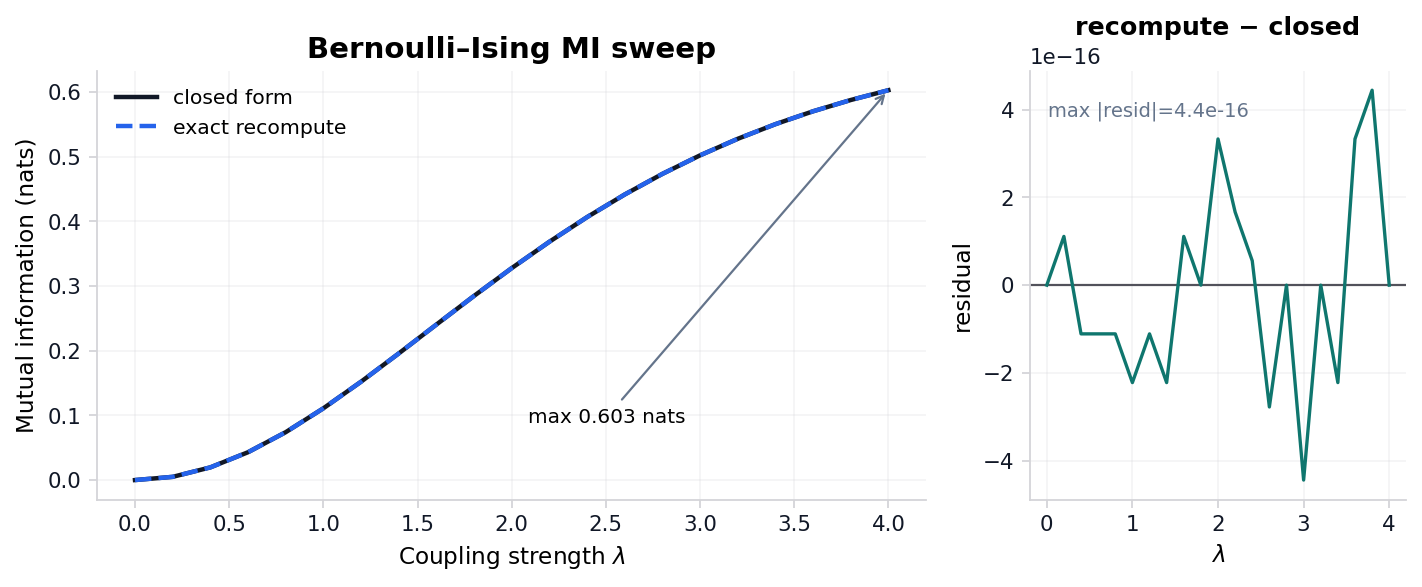
\includegraphics[width=0.9\linewidth,height=0.5\textheight,keepaspectratio]{../figures/ising_mi_curve.png}

\emph{Reproduced from fig.~\ref{fig:ising_mi_curve}. Closed-form
\(I(\lambda)\) and an independent exact recomputation via total
correlation for the symmetric Bernoulli-Ising toy across 21 grid points
up to \(\lambda_{\max}\) = 4; grid maximum 0.6031 nats. Both estimators
are deterministic (no sampling), so the right panel is a
cross-implementation agreement check (max residual 0 nats), not a
sampling residual.}

\newpage

\section{Free-energy decomposition}\label{sec:results_free_energy}

Free energy against the entangled prior is evaluated along the same
\(\lambda\) grid used for the MI sweep
(fig.~\ref{fig:free_energy_curve}). Against the \emph{entangled} prior
the entangled posterior is the exact variational minimizer, so its free
energy is identically zero; the Theorem-5.1 decomposition then splits
that zero into per-stream marginal free energies, a coupling-cost term,
a coupling-prior term, and a total-correlation gain. For the symmetric
toy with uniform marginals the coupling-prior term equals
\(-I(\lambda)\) and exactly cancels the total-correlation gain
\(+I(\lambda)\) --- an exact cancellation the merged invariant suite
checks (12/12 pass). The curve in fig.~\ref{fig:free_energy_curve}
instead reports free energy against the \emph{mean-field} prior: its
minimum at \(\lambda=0\) is where the entangled posterior coincides with
the factorized mean-field product, and any \(\lambda>0\) raises the free
energy as coupling pulls the posterior away from that independent prior.

Saturation MI (grid maximum on the measured \(\lambda\) sweep): 0.6031
nats.

\begin{figure}
\centering
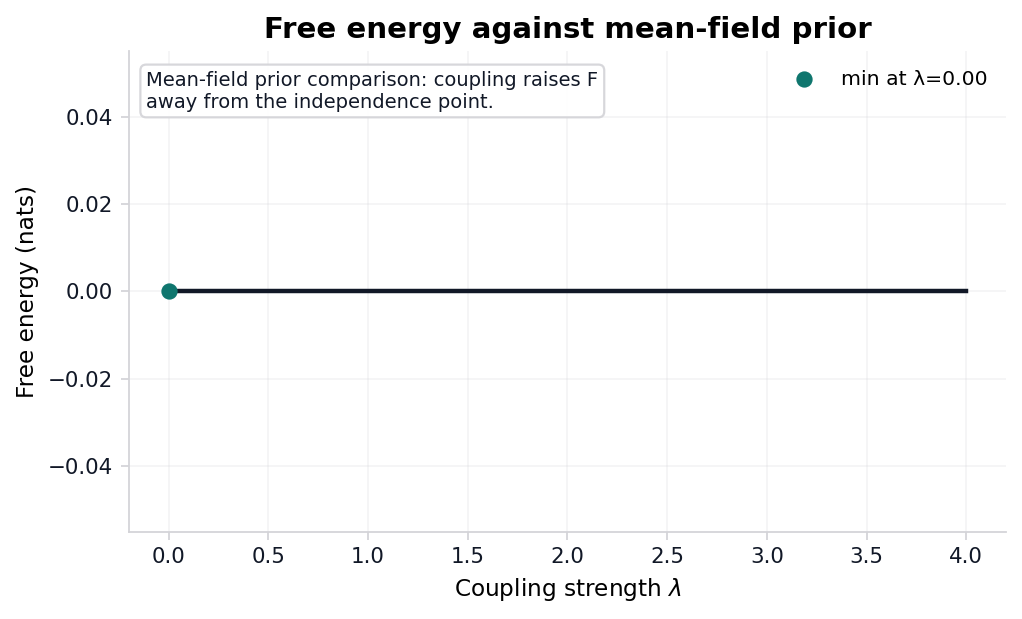
\includegraphics[width=0.9\linewidth,height=0.5\textheight,keepaspectratio,alt={Free energy of the entangled posterior relative to the mean-field prior across the hyperparameter sweep (grid points 21); relative to the entangled prior, the same posterior has identically zero free energy.}]{../figures/free_energy_curve.png}
\caption{Free energy of the entangled posterior relative to the
mean-field prior across the hyperparameter sweep (grid points 21);
relative to the entangled prior, the same posterior has identically zero
free energy.}\label{fig:free_energy_curve}
\end{figure}

\newpage

\section{T-maze active-inference rollout}\label{sec:results_si_tmaze}

The pymdp harness rolls out a T-maze active-inference agent in
\texttt{state\_inference} mode with planning horizon 2. The default
\texttt{state\_inference} mode is belief filtering with a goal-seeking
action rule; sophisticated policy inference (an expected-free-energy
policy posterior) is selectable via \breaktt{mode:\ policy\_inference}
(sec.~\ref{sec:methods_pymdp}). Summary metrics land in
\breaktt{output/data/si\_tmaze\_summary.json}.

Steps recorded: 2. Mean belief entropy: 0.3251. Belief entropy over the
rollout is traced in fig.~\ref{fig:si_belief_entropy_curve}; the paired
observation and action indices are in
fig.~\ref{fig:si_obs_action_trace}.
\breaktt{output/data/analysis\_statistics.json} now records the trace as
a small statistical object rather than a caption-only trace: action
switches 1 times (rate 1.000 over adjacent steps), observation diversity
is 1, entropy drop is 0.0000 nats from first to terminal step, and the
saved trace/summary step counts agree: \texttt{true} with finite entropy
values \texttt{true}. The default \texttt{state\_inference} mode runs
pymdp \texttt{infer\_states} and \textbf{reports} the resulting
posterior (belief entropy and the state-1 marginal), but the action is
chosen by an open-loop scripted rule on the observation index --- not by
the posterior --- so the inferred belief here is observed, not acted on.
Under the toy transition model, expected-free-energy policy inference
reaches the goal in 1 of its rows versus 2 for the scripted
state-inference rule: no behavioral advantage on this two-state,
horizon-2 maze, which is the measured content of the
deliberately-too-small claim.

Policy-comparison rows: 4 across state-inference and policy-inference
modes; goal-reaching rows: 3. These rows are internal toy consistency
checks under finite-horizon discrete active-inference assumptions
\citep{friston2021sophisticated, dacosta2023reward}, not comparisons
against external behavioral datasets. Graph-world extension rows: 4 over
4 nodes, with goal-reached flag 1.

The expected free energy that scores those policies decomposes in closed
form (fig.~\ref{fig:efe_decomposition}). Across the 4 length-2 policies
on the T-maze generative model, the expected-free-energy-minimising
policy is \texttt{00} with \(G\) = 2.2539 nats, splitting into risk
1.6037 (the pragmatic deviation of predicted outcomes from preferences)
and ambiguity 0.6502 (the expected likelihood entropy) nats. The same
\(G\) splits equivalently into pragmatic value -2.2539 (expected
log-preference) and epistemic value 0.0000 (state-outcome mutual
information) nats --- the term that drives information-seeking. The two
forms are exactly equal: risk + ambiguity + pragmatic + epistemic
vanishes to within 0.0e+00 across every policy, the action-selection
twin of the analytical free-energy decomposition identity
(sec.~\ref{sec:results_free_energy}).

Precision controls how sharply that expected free energy is acted on:
the policy posterior is the softmax-weighted
\(q(\pi) \propto \exp(-\gamma\,G(\pi))\), and sweeping the inverse
temperature \(\gamma\) across 33 grid points up to 16 sharpens it
monotonically (fig.~\ref{fig:precision_sweep}). Posterior entropy falls
from \(\ln 4\) at \(\gamma\)=0 to 1.1458 nats at \(\gamma\)=1, then
saturates at the floor 0.6931 nats rather than reaching zero: the
absorbing goal makes the second action irrelevant once reached, so 2
policies tie at the expected-free-energy minimum and precision
concentrates mass on that optimal \emph{set}, not a single policy. By
that honest criterion selection becomes effectively deterministic ---
optimal-set mass exceeding 0.99 --- at \(\gamma\)=3.

The minimal two-state maze above is, by construction, too small for
information-seeking to matter: the reward location is observable from
the start, so a greedy pragmatic rule and an expected-free-energy rule
reach the goal equally often. The cue-then-reward variant
(fig.~\ref{fig:cue_tmaze_advantage}) removes that degeneracy. Across 8
joint position-by-context states the reward location is an uninformative
latent (50/50 at the start) that is hidden until the agent visits a CUE
location, at which point a single sample resolves it: the cue carries
0.6931 nats of information (\(= \ln 2\), the entropy of the unknown
context). An agent that samples the cue and then takes the contingent
arm reaches reward with expected log-preference -0.0538 nats, against
-4.0538 nats for a greedy agent that commits to an arm before sampling
--- a measured behavioural advantage of 4.0000 nats that vanishes only
if epistemic value is removed from the objective. The advantage is
sophisticated, not flat: the closed-form flat decomposition of
sec.~\ref{sec:results_si_tmaze} scores the cue-first and greedy policies
as identical because it propagates beliefs through the transition model
without conditioning them on the cue observation. Resolving the latent
therefore requires an observation-conditioned (sophisticated-inference)
evaluation, and under that evaluation cue-sampling is strictly necessary
rather than merely available.

Planning is only half of the generative loop: the agent must also
\emph{learn} its likelihood. Placing a Dirichlet prior over each column
of \(A\) and accumulating observation-state counts \(c\) gives the
conjugate update \(pA \leftarrow pA + c\) with expected likelihood
\(E[A] = pA / \sum_o pA\) (fig.~\ref{fig:dirichlet_convergence}). Driven
by a fixed, sampling-free expected-count stream,
\(\mathrm{KL}(A_{\text{true}} \,\|\, A_{\text{learned}})\) falls
monotonically from 0.7361 nats at the uniform prior to 1.29e-03 nats,
reaching the convergence tolerance at update step 3. The learned
likelihood converges to the true generative model in closed form, the
inference-side twin of the EFE planning decomposition above.

Rollout trace: \breaktt{output/data/si\_tmaze\_trace.json}. JSONL run
log: \breaktt{output/logs/pymdp\_runs.jsonl}.

\begin{figure}
\centering
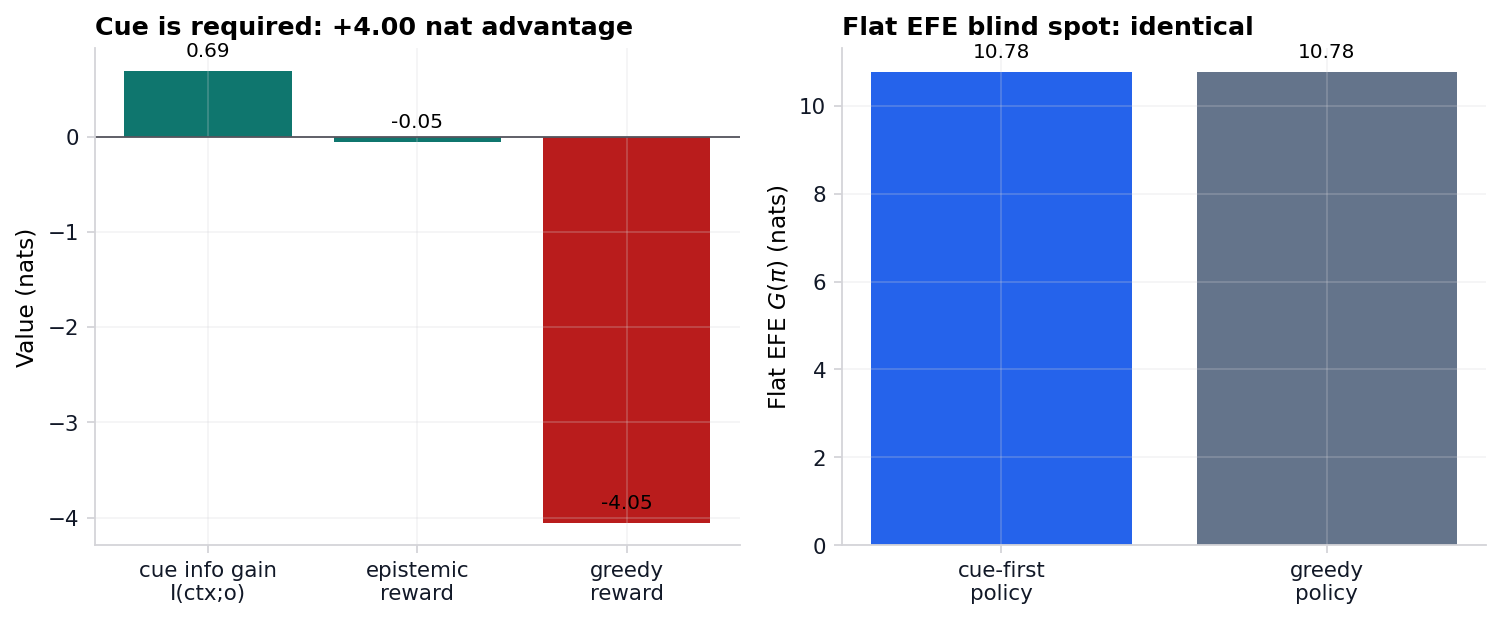
\includegraphics[width=0.95\linewidth,height=0.5\textheight,keepaspectratio,alt={Cue-then-reward T-maze where epistemic value is strictly necessary. Left: the cue carries 0.6931 nats of information and the cue-sampling agent reaches reward with a measured advantage of 4.0000 nats over a greedy agent. Right: flat Expected Free Energy scores the cue-first and greedy policies identically (identical), so the sophisticated observation- conditioned evaluator is what makes information-seeking required. Closed form (no sampling).}]{../figures/cue_tmaze_advantage.png}
\caption{Cue-then-reward T-maze where epistemic value is strictly
necessary. Left: the cue carries 0.6931 nats of information and the
cue-sampling agent reaches reward with a measured advantage of 4.0000
nats over a greedy agent. Right: flat Expected Free Energy scores the
cue-first and greedy policies identically (identical), so the
sophisticated observation- conditioned evaluator is what makes
information-seeking required. Closed form (no
sampling).}\label{fig:cue_tmaze_advantage}
\end{figure}

\begin{figure}
\centering
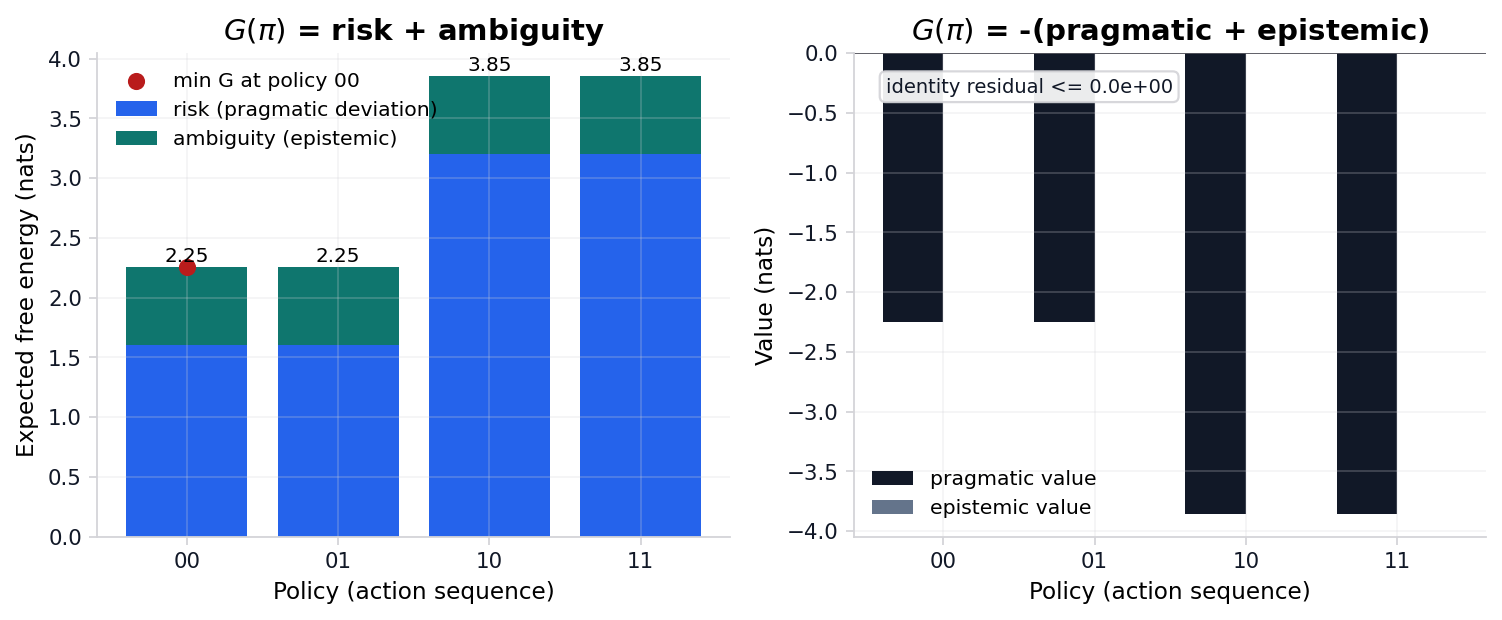
\includegraphics[width=0.95\linewidth,height=0.5\textheight,keepaspectratio,alt={Closed-form Expected Free Energy decomposition over the finite T-maze policies. Left: G(\textbackslash pi) = risk + ambiguity (stacked), with the goal-seeking minimiser marked. Right: the pragmatic and epistemic values, which sum to -G(\textbackslash pi). Both forms are computed in closed form (no sampling) and satisfy risk + ambiguity + pragmatic + epistemic = 0 to machine precision.}]{../figures/efe_decomposition.png}
\caption{Closed-form Expected Free Energy decomposition over the finite
T-maze policies. Left: \(G(\pi)\) = risk + ambiguity (stacked), with the
goal-seeking minimiser marked. Right: the pragmatic and epistemic
values, which sum to \(-G(\pi)\). Both forms are computed in closed form
(no sampling) and satisfy risk + ambiguity + pragmatic + epistemic = 0
to machine precision.}\label{fig:efe_decomposition}
\end{figure}

\begin{figure}
\centering
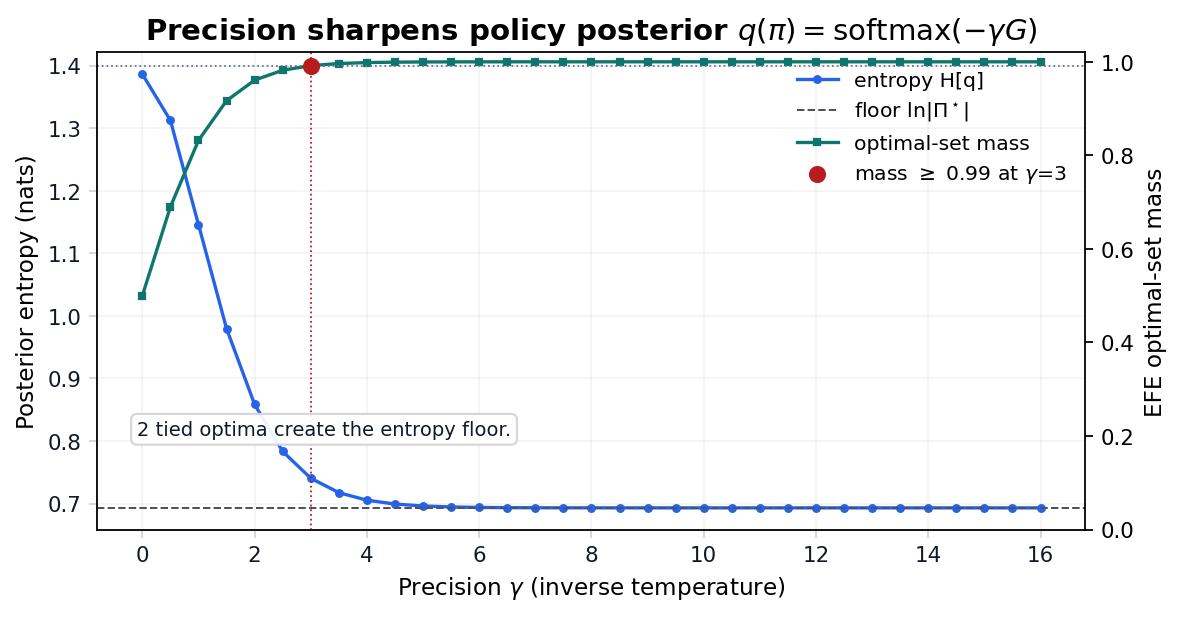
\includegraphics[width=0.9\linewidth,height=0.5\textheight,keepaspectratio,alt={Precision sweep over the closed-form T-maze policy posterior q(\textbackslash pi)\textbackslash propto\textbackslash exp(-\textbackslash gamma G) across 33 grid points up to \textbackslash gamma=16. Entropy falls from \textbackslash ln 4 to the \textbackslash ln|\textbackslash Pi\^{}\textbackslash star|{} floor (2 tied optima, second action irrelevant under the absorbing goal); the optimal-set mass crosses 0.99 at \textbackslash gamma=3. Entropy at \textbackslash gamma=1 is 1.1458 nats. Computed in closed form (no sampling).}]{../figures/precision_sweep.png}
\caption{Precision sweep over the closed-form T-maze policy posterior
\(q(\pi)\propto\exp(-\gamma G)\) across 33 grid points up to
\(\gamma\)=16. Entropy falls from \(\ln 4\) to the \(\ln|\Pi^\star|\)
floor (2 tied optima, second action irrelevant under the absorbing
goal); the optimal-set mass crosses 0.99 at \(\gamma\)=3. Entropy at
\(\gamma\)=1 is 1.1458 nats. Computed in closed form (no
sampling).}\label{fig:precision_sweep}
\end{figure}

\begin{figure}
\centering
\includegraphics[width=0.85\linewidth,height=0.5\textheight,keepaspectratio,alt={Dirichlet model learning: KL(A\_\{\textbackslash text\{true\}\} \textbackslash,\textbackslash|\textbackslash, A\_\{\textbackslash text\{learned\}\}) versus concentration-update step. The expected likelihood E{[}A{]} = pA / \textbackslash sum\_o pA converges monotonically to the true generative likelihood; the run reaches the convergence tolerance at step 3 with final KL 1.29e-03 nats. Deterministic (no sampling), so the curve is byte-reproducible.}]{../figures/dirichlet_convergence.png}
\caption{Dirichlet model learning:
KL\((A_{\text{true}} \,\|\, A_{\text{learned}})\) versus
concentration-update step. The expected likelihood
\(E[A] = pA / \sum_o pA\) converges monotonically to the true generative
likelihood; the run reaches the convergence tolerance at step 3 with
final KL 1.29e-03 nats. Deterministic (no sampling), so the curve is
byte-reproducible.}\label{fig:dirichlet_convergence}
\end{figure}

\begin{figure}
\centering
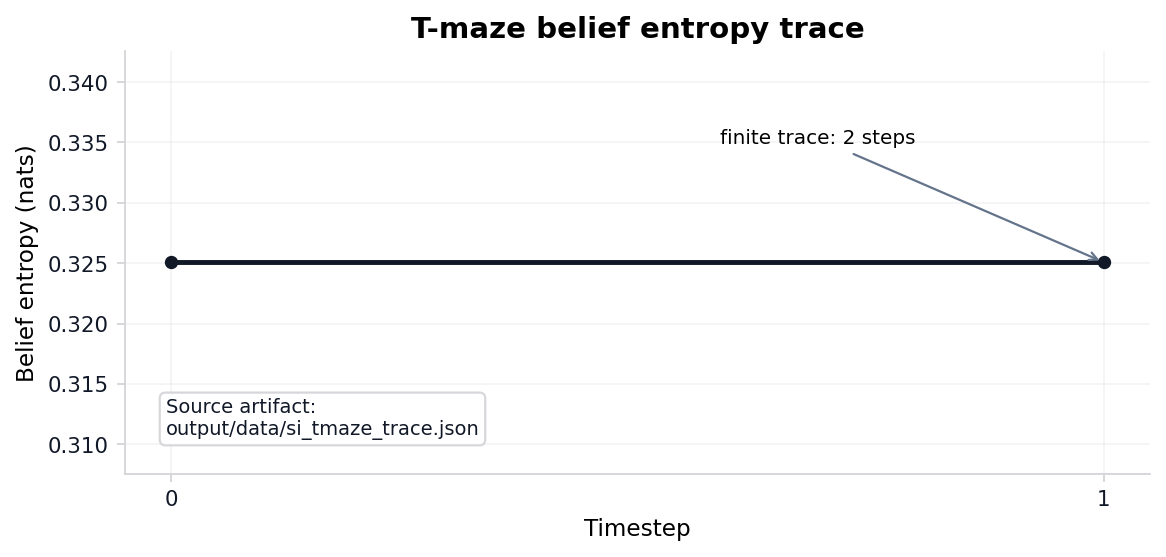
\includegraphics[width=0.9\linewidth,height=0.5\textheight,keepaspectratio,alt={Belief entropy over time for the T-maze rollout (mean 0.3251 nats).}]{../figures/si_belief_entropy_curve.png}
\caption{Belief entropy over time for the T-maze rollout (mean 0.3251
nats).}\label{fig:si_belief_entropy_curve}
\end{figure}

\begin{figure}
\centering
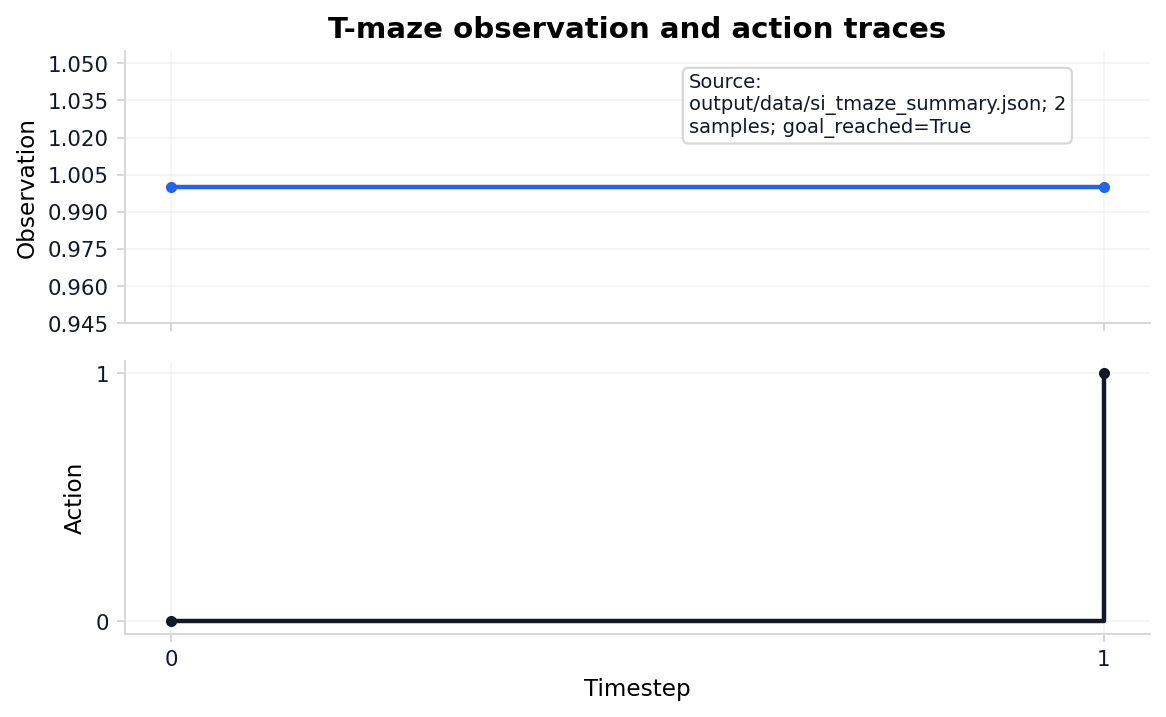
\includegraphics[width=0.9\linewidth,height=0.5\textheight,keepaspectratio,alt={Observation and action traces for the T-maze rollout (action diversity 2).}]{../figures/si_obs_action_trace.png}
\caption{Observation and action traces for the T-maze rollout (action
diversity 2).}\label{fig:si_obs_action_trace}
\end{figure}

\begin{figure}
\centering
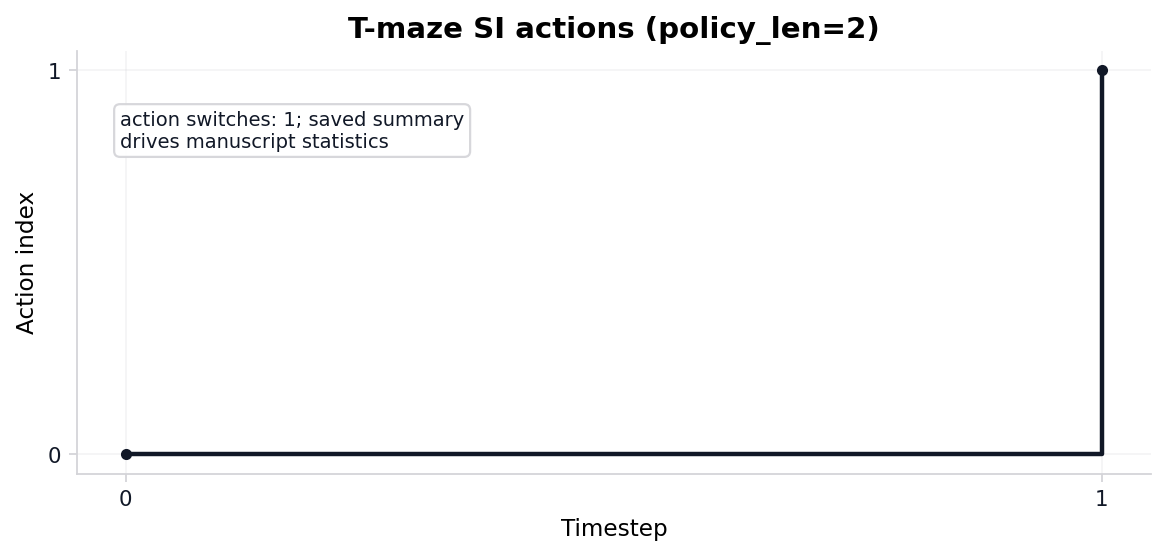
\includegraphics[width=0.9\linewidth,height=0.5\textheight,keepaspectratio,alt={Discrete action index over time for the pymdp T-maze rollout (policy length 2).}]{../figures/si_tmaze_actions.png}
\caption{Discrete action index over time for the pymdp T-maze rollout
(policy length 2).}\label{fig:si_tmaze_actions}
\end{figure}

\newpage

\section{Validation invariants}\label{sec:results_invariants}

The analytical invariant registry runs before PDF rendering
(sec.~\ref{sec:methods_analytical}). On a clean checkout \textbf{12 /
12} checks pass in the merged validation report, which records
simulation invariants when the pymdp harness ran
(sec.~\ref{sec:results_si_tmaze}).

fig.~\ref{fig:invariant_dashboard} lists each analytical and simulation
gate; failures block publication artifacts. See
sec.~\ref{sec:methods_sheaf} for how invariant counts hydrate manuscript
tokens.

Simulation invariants merge into the analytical report after the pymdp
harness runs (sec.~\ref{sec:results_si_tmaze}).
fig.~\ref{fig:invariant_dashboard} summarizes pass/fail status for both
domains on the clean tree.

The replay matrix exposes deterministic rerun comparison as table data
rather than prose. It contains 13 producer rows, uses explicit
replay-or-fingerprint methods, and every row must match its saved
artifact hash (\texttt{true}).

The \texttt{sensitivity} fragment binds the deterministic toy sweep to
the canonical sheaf track. \breaktt{output/data/sensitivity\_sweep.json}
contains 96 cells across toy parameters, policy modes, seeds, horizons,
and graph topologies; the hydrated flag \texttt{true} is the only
manuscript claim about coverage.

The companion \breaktt{output/data/si\_policy\_grid.json} records
measured policy-mode rows derived from
\breaktt{si\_policy\_comparison.json}, not a synthetic grid. Missing
cells fail the artifact schema before they can become prose; the
topology trace artifact contributes 4 deterministic topology traces.

The \texttt{uncertainty} fragment reports only normalized toy summaries.
\breaktt{output/data/uncertainty\_summary.json} contains 12 belief and
policy-posterior rows plus 3 finite entropy bins, and \texttt{true} is
false if any posterior row fails to sum to one within the deterministic
tolerance.

Policy uncertainty is recorded in generated policy artifacts rather than
hand-entered into the manuscript. The posterior grid contributes 5
available posterior rows; the EFE values artifact reports
availability-or-measured-fallback flag 1. The fragment is therefore a
validation surface, not an empirical uncertainty claim.

The \texttt{benchmark} fragment adds a compact toy matrix over the
Bernoulli, T-maze, and graph-world artifacts.
\breaktt{output/data/toy\_benchmark\_matrix.json} reports 3 model rows
and \texttt{true} only when each row names an artifact, metric, and
passing gate.

The matrix is scoped to deterministic exemplar models. It is useful as a
cross-track smoke test, not as a performance benchmark for biological or
deployed systems.

\begin{figure}
\centering
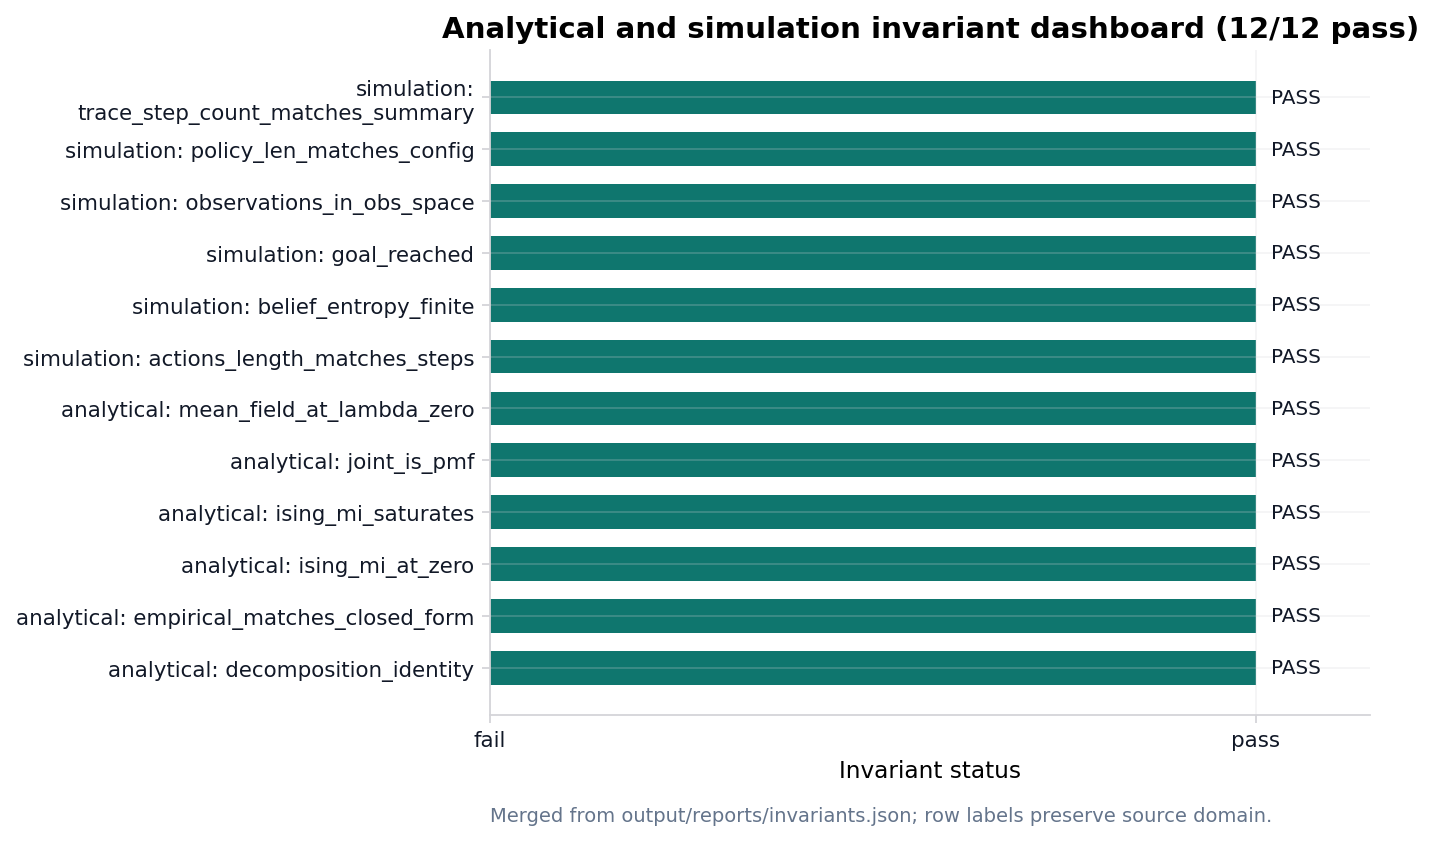
\includegraphics[width=0.9\linewidth,height=0.5\textheight,keepaspectratio,alt={Invariant dashboard: 12 / 12 merged analytical and simulation checks from the validation registry.}]{../figures/invariant_dashboard.png}
\caption{Invariant dashboard: 12 / 12 merged analytical and simulation
checks from the validation registry.}\label{fig:invariant_dashboard}
\end{figure}

\subsubsection{State-space catalog
track}\label{state-space-catalog-track}

The \breaktt{state\_space\_catalog} track enumerates finite state spaces,
action spaces, and policy counts for the deterministic toy models. The
catalog artifact is \breaktt{output/data/state\_space\_catalog.json}: it
currently records 6 rows, with finite-space status \texttt{true}.

\subsubsection{Causal ablation track}\label{causal-ablation-track}

The \texttt{causal\_ablation} track records deterministic toy ablations
over finite preferences, likelihood-noise settings, and graph-topology
perturbations. The matrix artifact is
\breaktt{output/data/causal\_ablation\_matrix.json}: it currently records
36 cells, with complete-grid status \texttt{true}.

\newpage

\phantomsection
\addcontentsline{toc}{section}{Discussion}
\section*{Discussion}

\section{Limitations and outlook}\label{sec:discussion_outlook}

\subsection{What this demonstrates}\label{what-this-demonstrates}

The result of this manuscript is a \emph{discipline}, not a domain
claim: across three toy models every reported number is hydrated from a
generated artifact, 6 sheaf axioms are machine-checked before
composition, and 25 negative controls keep each failure path live. That
posture follows the caution that FEP and active-inference formalisms
need explicit methodological scope before they become empirical brain
claims \citep{gershman2019fepbrain}. No statistic, figure, or
cross-track claim here can drift from its artifact without failing a
gate before the PDF is built.

\subsection{Limitations}\label{limitations}

The Bernoulli--Ising toy, T-maze harness, and sheaf composition model
are pedagogical. They validate analytical consistency, artifact wiring,
renderer dispatch, and manuscript hydration, not empirical claims about
biological agents. Default pymdp mode is \texttt{state\_inference} with
planning horizon 2; the policy-comparison artifact exposes
policy-inference rows without changing the default rollout
(sec.~\ref{sec:methods_pymdp}).

\subsection{Sheaf audit and outlook}\label{sheaf-audit-and-outlook}

sec.~\ref{sec:sheaf_coverage} and sec.~\ref{sec:appendix_full_sheaf}
make binding state auditable under strict compose validation
(sec.~\ref{sec:methods_sheaf}). Pipeline extensions in
\texttt{tracks.yaml} \breaktt{extension\_tracks} now write deterministic
artifacts: a belief GIF via \breaktt{render\_animation.py} and
graph-world SI summary/trace via \breaktt{simulate\_si\_graph\_world.py}.
The appendix row already binds an \texttt{animation} sheaf fragment
without new manifest rows.

Sweep RMSE 0 nats and SI goal reached 1 summarize measured agreement on
the declared grids and rollout. Future work includes full
expected-free-energy policy selection, richer graph-world rollouts, and
expanded Lean proofs beyond the boundary witnesses in
sec.~\ref{sec:methods_lean}.

The discussion ontology binds \breaktt{coverage\_semantics} to the audit
matrix in sec.~\ref{sec:sheaf_coverage}, \breaktt{pedagogical\_scope} to
the non-empirical scope of the toy models, and
\breaktt{state\_inference\_mode} to the pymdp harness contract in
sec.~\ref{sec:methods_pymdp}.

Measured pymdp rollout (\texttt{state\_inference}, config hash
\breaktt{81eb061f43b7bfd7}): mean belief entropy 0.3251 nats over 2
steps; goal reached flag 1; action diversity 2.

Analytical sweep residual RMSE 0 nats (max residual 0). Coverage audit:
95 present / 95 bound / 0 missing cells on the IMRAD matrix.

The scholarship matrix is also a scope-control device. It separates
conceptual lineage from measured evidence: cited sources explain why the
toy models are relevant, while generated artifacts decide every
numerical, figure, and gate claim. That split keeps the paper from
converting background authority into an unsupported empirical result.

Sophisticated Learning is therefore cited as a future-only
parameter-learning direction \citep{hodson2023sophisticatedlearning}. It
does not change the current T-maze state-inference default, does not
promote an active-learning adapter, and does not alter the blocked
major-scope ladder for empirical or non-toy claims.

\subsubsection{Ontology bindings}\label{ontology-bindings-3}

\begin{itemize}
\tightlist
\item
  \breaktt{coverage\_semantics} \texorpdfstring{\ensuremath{\to}}{->} \textbf{Coverage matrix semantics}
\item
  \breaktt{pedagogical\_scope} \texorpdfstring{\ensuremath{\to}}{->} \textbf{Pedagogical scope}
\item
  \breaktt{state\_inference\_mode} \texorpdfstring{\ensuremath{\to}}{->} \textbf{State inference harness}
\end{itemize}

\subsubsection{Release notes evidence
track}\label{release-notes-evidence-track}

The \texttt{release\_notes} track keeps release-language claims
source-backed by validation, semantic, and bundle artifacts. Its
evidence artifact is
\breaktt{output/reports/release\_notes\_evidence.json}: it currently
records 3 rows, with source-backed status \texttt{true}.

\newpage

\phantomsection
\addcontentsline{toc}{section}{Appendix}
\section*{Appendix}

\section{Appendix: full track coverage}\label{sec:appendix_full_sheaf}

This section is the \textbf{composability proof} for the
manifest-indexed sheaf model: all 33 appendix-bound fragment tracks
render into one flat manuscript section without section-specific compose
branches. The registry defines 34 composable types; optional
\texttt{layers} is methods-only and excluded from this row. The
\texttt{animation} fragment is bound here as an optional registry type
alongside the live proof, simulation, formal, notation,
validation-spine, integration, audit, finite-catalog, ablation, license,
release-evidence, scholarship, assumption-index, delta, and staleness
tracks.

The proof is a publication-systems check
(eq.~\ref{eq:appendix_track_count}). It demonstrates that heterogeneous
fragments share one registry, manifest, renderer dispatch path, coverage
matrix, and hydration boundary; it does not assert that every track
carries equal scientific weight.

For each track \(t \in \mathcal{T}_{\mathrm{Full}}\), the appendix row
binds a fragment path \(f(t)\) and the composer emits
\texttt{\textless{}!-\/-\ sheaf-track:t\ -\/-\textgreater{}} before the
rendered body. Generated renderers such as \texttt{section\_figures} and
markdown renderers pass through the same \breaktt{resolve\_track\_body()}
dispatch, so the appendix exercises the common compose interface rather
than a bespoke appendix path.

\begin{equation}\protect\phantomsection\label{eq:appendix_track_count}{
|\mathcal{T}_{\mathrm{Full}}| = 33
}\end{equation}

The fragment registry defines 34 composable track types; optional
\texttt{layers} is bound on the methods sheaf section only. Optional
\texttt{animation} is bound in this appendix proof; the deterministic
GIF artifact in \texttt{tracks.yaml} \breaktt{extension\_tracks} is
produced by the core analysis DAG and remains separate from this
fragment slot.

Because this appendix binds every non-optional appendix track plus
optional \texttt{animation}, it is the maximal publication stalk of the
coverage presheaf and exercises every publication renderer through the
common \breaktt{resolve\_track\_body()} dispatch. The same compose path
is gated by the 6 sheaf laws verified in sec.~\ref{sec:methods_sheaf}
(6/6 satisfied): the appendix section glues to a unique output
(separation), occupies the terminal position of the linear extension
under its own \texttt{appendix} group row (poset and gluing), binds only
well-typed fragments (typing), and owns every fragment path it
references (compositionality). No count in this appendix is
hand-written; all are injected from the registry-backed oracle.

Analytical sweep artifacts feed sec.~\ref{sec:results_mi_sweep} and
sec.~\ref{sec:results_invariants}; simulation invariants merge after
sec.~\ref{sec:results_si_tmaze}. No additional path listing is required
beyond those Results sections.

The appendix \breaktt{assumption\_index} row points to
\breaktt{output/data/analytical\_assumption\_index.json}. It binds 7
finite Bernoulli-Ising assumption rows to 7 equation identifiers and
generated artifacts, with indexed status \texttt{true}.

The point is to make analytical signposting mechanical. If an equation
is added without an assumption row, or if a row loses its evidence
artifact, the index gate fails and the manuscript cannot present the
equation as part of the validated finite toy proof surface.

pymdp harness summary: \breaktt{output/data/si\_tmaze\_summary.json}
(mean belief entropy, action trace). Runtime diagnostics:
\breaktt{output/reports/pymdp\_runtime\_diagnostics.json} (known warnings
4, unexpected warnings 0). Policy posterior grid:
\breaktt{output/data/pymdp\_policy\_posterior\_grid.json} (10 rows). Full
log: \breaktt{output/logs/pymdp\_runs.jsonl}.

\breaktt{sheaf-track:interop} binds
\breaktt{output/data/interop\_roundtrip\_report.json},
\breaktt{output/data/gnn\_roundtrip\_report.json},
\breaktt{output/reports/gnn\_lint\_report.json}, and ontology profile
artifacts into the appendix proof row. The appendix claim is exactly 2
checks with lossless status \texttt{true}.

The appendix provenance fragment points to
\breaktt{output/data/artifact\_provenance.json}, the canonical artifact
that records required toy artifact hashes, producer scripts, source
commit, deterministic seeds, config digests, and 5 bundle rows.

\breaktt{replay\_matrix.json} provides the appendix proof for
deterministic replay: 13 producer replay/fingerprint rows with matched
status \texttt{true}.

The appendix counterexample fragment points to
\breaktt{output/reports/counterexample\_matrix.json}, the
expected-failure matrix that keeps promoted validation gates
falsifiable. It currently records 25 known-bad fixtures, and the
hydrated pass flag is \texttt{1}, meaning those fixtures are expected to
fail rather than sneak through a positive-control gate.

This row is the negative-control ledger for the sheaf. Each
counterexample names a promoted track, target validation gate, mutation,
and observed expected-failure status. A new live track without a
counterexample row is therefore visibly incomplete in the
track-improvement scope.

\breaktt{sheaf-track:adversarial\_audit} binds
\breaktt{output/reports/adversarial\_audit.json},
\breaktt{output/reports/scope\_boundary\_audit.json}, and claim-audit
outputs. The appendix claim is exactly 25 expected-failure rows with
documented status \texttt{true} and known-bad-passing count 0.

\breaktt{evidence\_field\_index.json} provides the appendix proof for
field-level claim evidence: 97 mapped fields with status \texttt{true}.

\breaktt{release\_bundle\_manifest.json} provides the appendix proof for
required deliverables: 38 artifacts with source-present status
\texttt{true}.

\breaktt{artifact\_contract\_index.json} is the appendix-level
cross-artifact concordance proof. It rederives 85 rows from the live
semantic producer map and release-bundle parity rows, with row-complete
flag \texttt{true} and copied-parity flag \texttt{true}.

\breaktt{validation\_gate\_index.json} provides the appendix proof for
gate ergonomics: 26 indexed gates. \breaktt{track\_lane\_matrix.json}
adds 32 pipeline-to-sheaf rows with completion flag \texttt{true}.

\subsubsection{Appendix track: artifact
diffoscope}\label{appendix-track-artifact-diffoscope}

\breaktt{artifact\_diffoscope} binds
\breaktt{output/reports/artifact\_diffoscope.json} into the full sheaf
appendix. Rows: 41. All equal: \texttt{true}.

This diffoscope is deliberately narrow and reproducibility-facing. For
each non-cyclic generated artifact, it compares the saved provenance
digest to the live file digest at validation time. The validator
re-derives equality from the rows, so a stale \breaktt{all\_equal:\ true}
summary cannot hide one changed artifact.

The row count is not a decoration; it is the number of artifact
fingerprints that survived cycle exclusion and therefore can be compared
directly. This keeps the release bundle honest about mutable files while
avoiding self-referential hashes for artifacts that necessarily include
their own provenance.

\subsubsection{Appendix track: artifact
license}\label{appendix-track-artifact-license}

\breaktt{artifact\_license} binds
\breaktt{output/reports/artifact\_license\_audit.json} into the full
sheaf appendix. Rows: 85. All safe: \texttt{true}.

The license audit classifies each generated or source-backed artifact
under the public exemplar's configured license boundary. It is
intentionally conservative: generated local outputs and project-owned
source files pass, while an artifact outside those public source kinds
would need an explicit provenance and license row before it could
support a manuscript claim.

This is also where the blocked empirical-adapter boundary matters.
Private, restricted, or network-derived data are not smuggled in as
evidence; they remain blocked until privacy, licensing, typed-claim,
semantic, and negative-control gates are implemented in the same
artifact path.

\breaktt{sheaf-track:scholarship} binds
\breaktt{output/data/scholarship\_source\_matrix.json} into the appendix
proof row. The appendix claim is exactly 21 connected source rows with
connected status \texttt{true}; each row names a bibliography key,
locator, manuscript citation status, declared consumer sections, method
role, registered track set, evidence artifact, and claim-boundary
statement. The row set includes 3 quantitative/statistical or
visualization-quality method roles, including 7 statistically backed
figures with bridge status \texttt{true}. The explicit crosswalk has 7
rows and 9 statistical source links; every row is referenced in the
manuscript (\texttt{true}), and every such reference section is
manifest-bound to sheaf tracks (\texttt{true}) with a visualization
track present (\texttt{true}). This binds statistics and figure-quality
claims to generated artifacts rather than bibliography authority. The
scholarship matrix itself also records manuscript citation presence
(\texttt{true}), declared-section citation overlap count (19),
scope-guarded boundaries (\texttt{true}), and live row re-derivation
(\texttt{true}), which makes forged aggregate source-connectivity flags
fail at the validation boundary.

The visualization registry is also now a paper-integration object: role
metadata complete \texttt{true}, paper claims complete \texttt{true},
and section bindings complete \texttt{true}. Those flags are read from
the saved visualization-quality audit and then rechecked through the
semantic sheaf restrictions.

The appendix includes the security posture as a release-boundary proof
object. Each row in
\breaktt{output/reports/security\_posture\_audit.json} has evidence
artifacts, validators, a scoped boundary statement, and a
negative-control identifier. The negative controls target the verifier
failure modes a well-resourced adversary would prefer: aggregate
forgery, untracked credentials, network-derived evidence, private-data
leakage, unsigned production-release claims, and production zero-trust
claims without a runtime identity plane.

The posture is therefore defensive and local: it hardens this public
template against evidence laundering, artifact drift, secret exposure,
and false release claims while keeping production-only controls deferred
until a real deployment adds signed provenance, SBOMs, identity-aware
access, telemetry, and incident response evidence.

\breaktt{sheaf-track:sensitivity} binds
\breaktt{output/data/sensitivity\_sweep.json}, measured
\breaktt{output/data/si\_policy\_grid.json}, compatibility-named EFE
values artifact \breaktt{output/data/si\_efe\_terms.json},
\breaktt{output/data/analytical\_observable\_sweep.json}, and graph-world
topology artifacts including
\breaktt{output/data/si\_graph\_world\_topology\_traces.json}. The
appendix claim is exactly 96 complete canonical grid cells.

\breaktt{sheaf-track:uncertainty} binds
\breaktt{output/data/uncertainty\_summary.json}. The appendix claim is
exactly 12 normalized rows across 3 entropy bins with status
\texttt{true}.

\breaktt{sheaf-track:benchmark} binds
\breaktt{output/data/toy\_benchmark\_matrix.json}. The appendix claim is
exactly 3 complete toy-model rows with status \texttt{true}.

The appendix \breaktt{manuscript\_staleness} row points to
\breaktt{output/reports/manuscript\_staleness\_report.json}. It checks
322 token bindings after hydration, including late audit variables, and
the pass flag is \texttt{true}.

This is the rendered-output side of the sheaf contract. Source fragments
may contain hydration placeholders, but the public manuscript must not;
the staleness report compares each token's generated value against the
resolved markdown so stale counts are caught after composition, not only
during source-file linting.

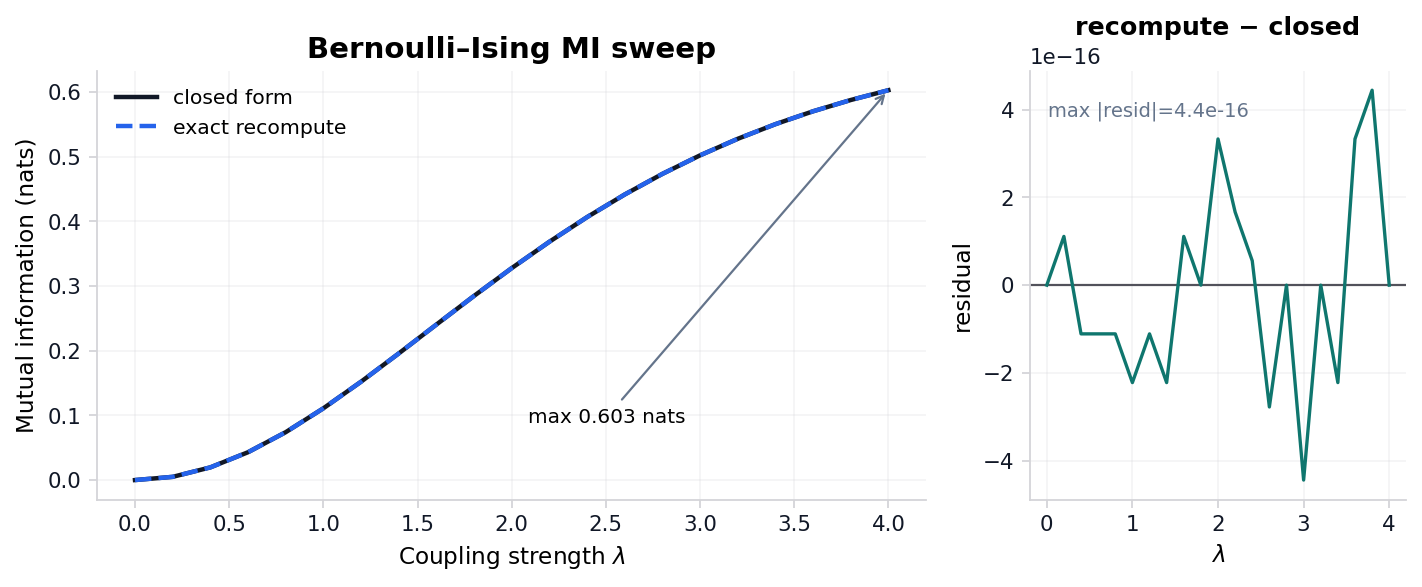
\includegraphics[width=0.9\linewidth,height=0.5\textheight,keepaspectratio]{../figures/ising_mi_curve.png}

\emph{Reproduced from fig.~\ref{fig:ising_mi_curve}. Closed-form
\(I(\lambda)\) and an independent exact recomputation via total
correlation for the symmetric Bernoulli-Ising toy across 21 grid points
up to \(\lambda_{\max}\) = 4; grid maximum 0.6031 nats. Both estimators
are deterministic (no sampling), so the right panel is a
cross-implementation agreement check (max residual 0 nats), not a
sampling residual.}

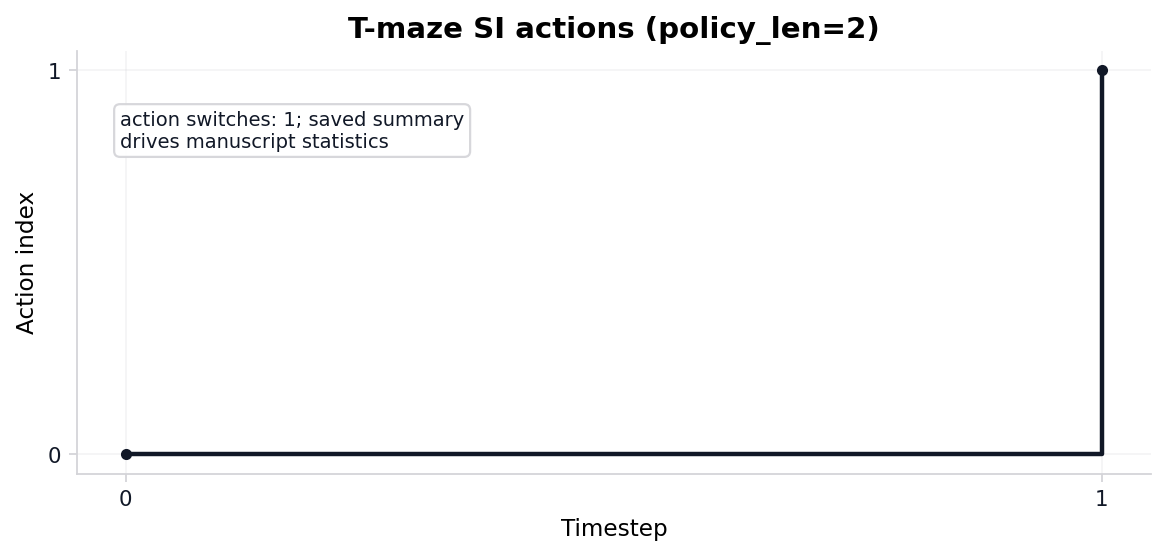
\includegraphics[width=0.9\linewidth,height=0.5\textheight,keepaspectratio]{../figures/si_tmaze_actions.png}

\emph{Reproduced from fig.~\ref{fig:si_tmaze_actions}. Discrete action
index over time for the pymdp T-maze rollout (policy length 2).}

\begin{figure}
\centering
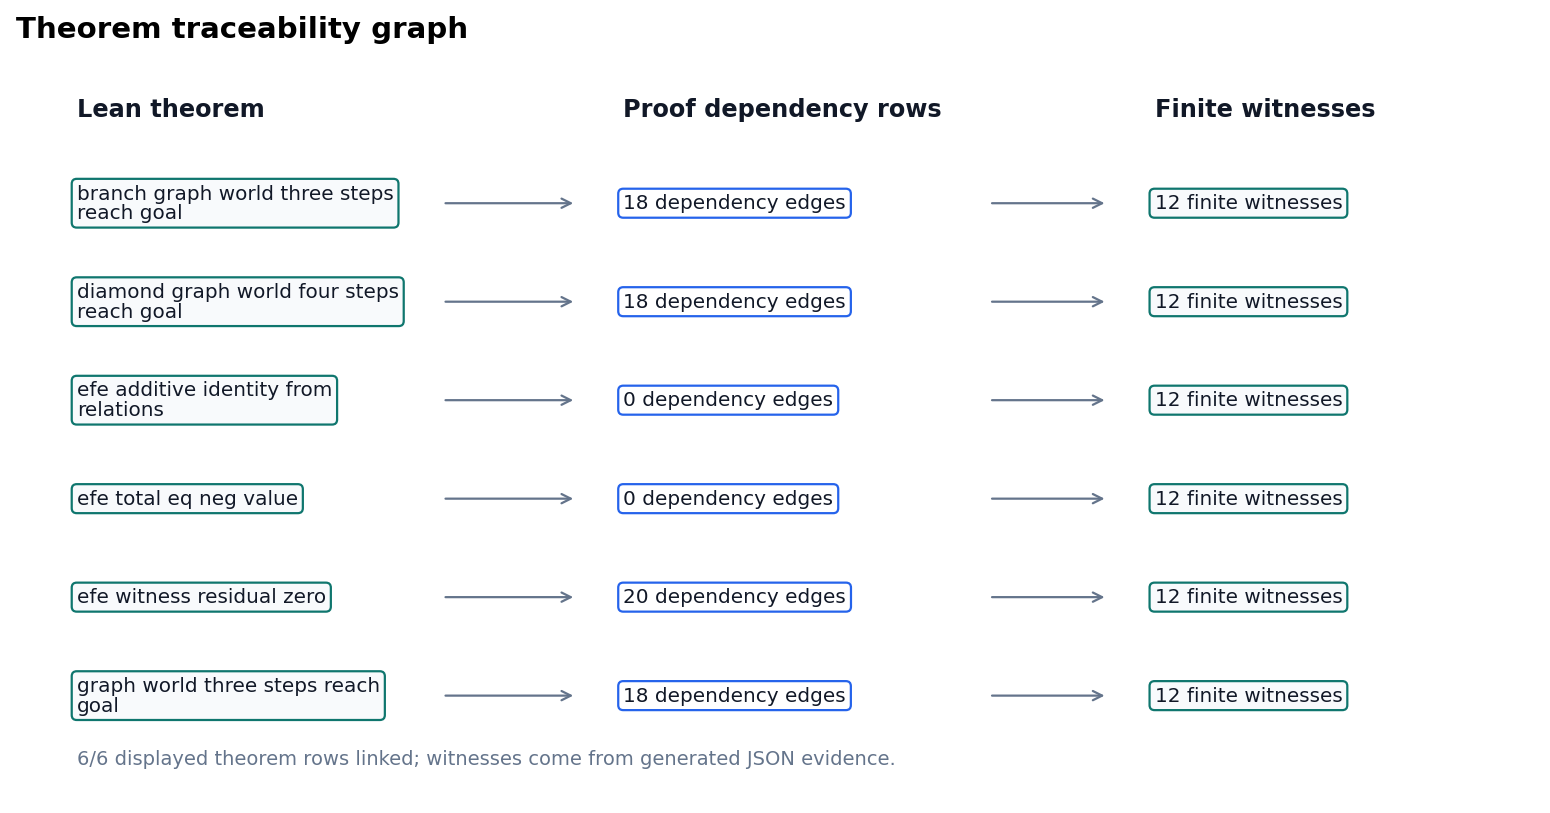
\includegraphics[width=0.95\linewidth,height=0.5\textheight,keepaspectratio,alt={Theorem traceability graph generated from 17 linked theorem rows and 207 proof-dependency edges.}]{../figures/theorem_traceability_graph.png}
\caption{Theorem traceability graph generated from 17 linked theorem
rows and 207 proof-dependency
edges.}\label{fig:theorem_traceability_graph}
\end{figure}

\begin{figure}
\centering
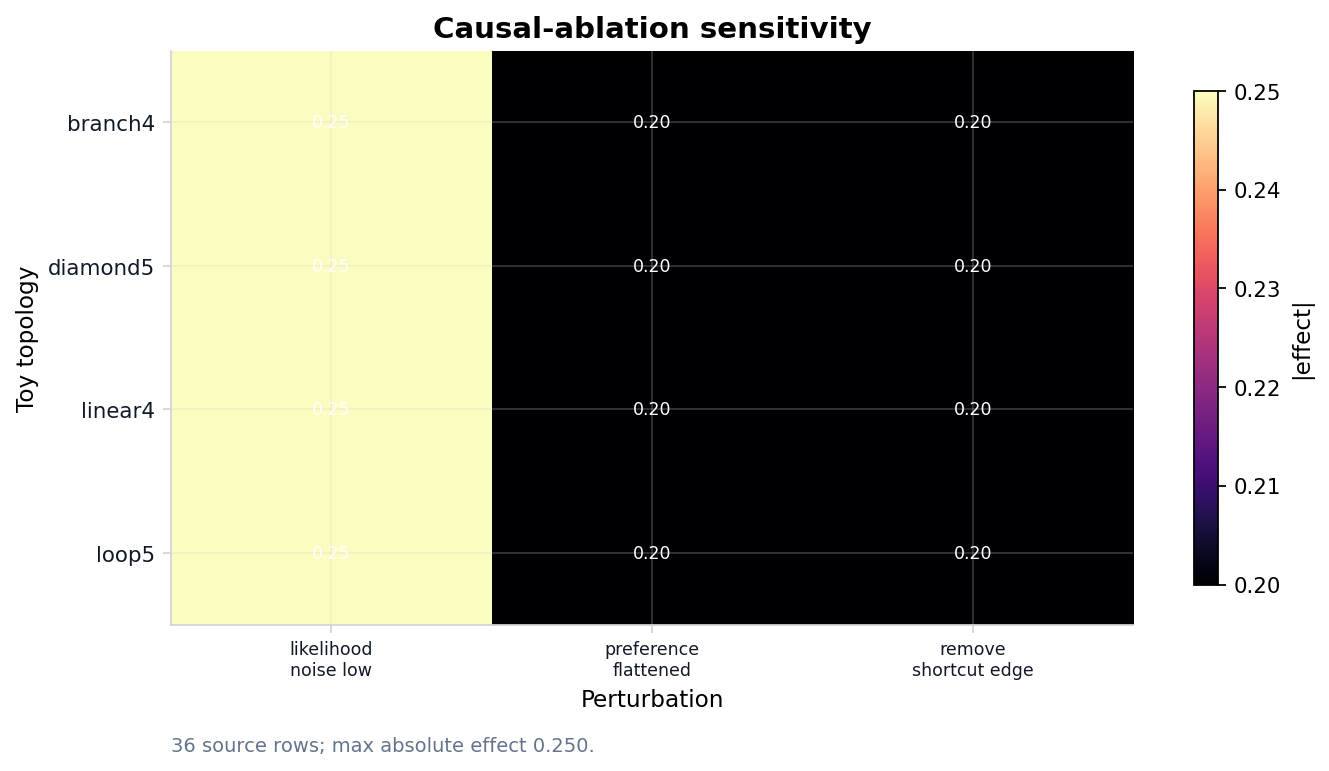
\includegraphics[width=0.92\linewidth,height=0.5\textheight,keepaspectratio,alt={Causal-ablation heatmap: 36 source-backed rows joined to sensitivity and uncertainty artifacts; all effects source-backed: true.}]{../figures/causal_ablation_heatmap.png}
\caption{Causal-ablation heatmap: 36 source-backed rows joined to
sensitivity and uncertainty artifacts; all effects source-backed:
true.}\label{fig:causal_ablation_heatmap}
\end{figure}

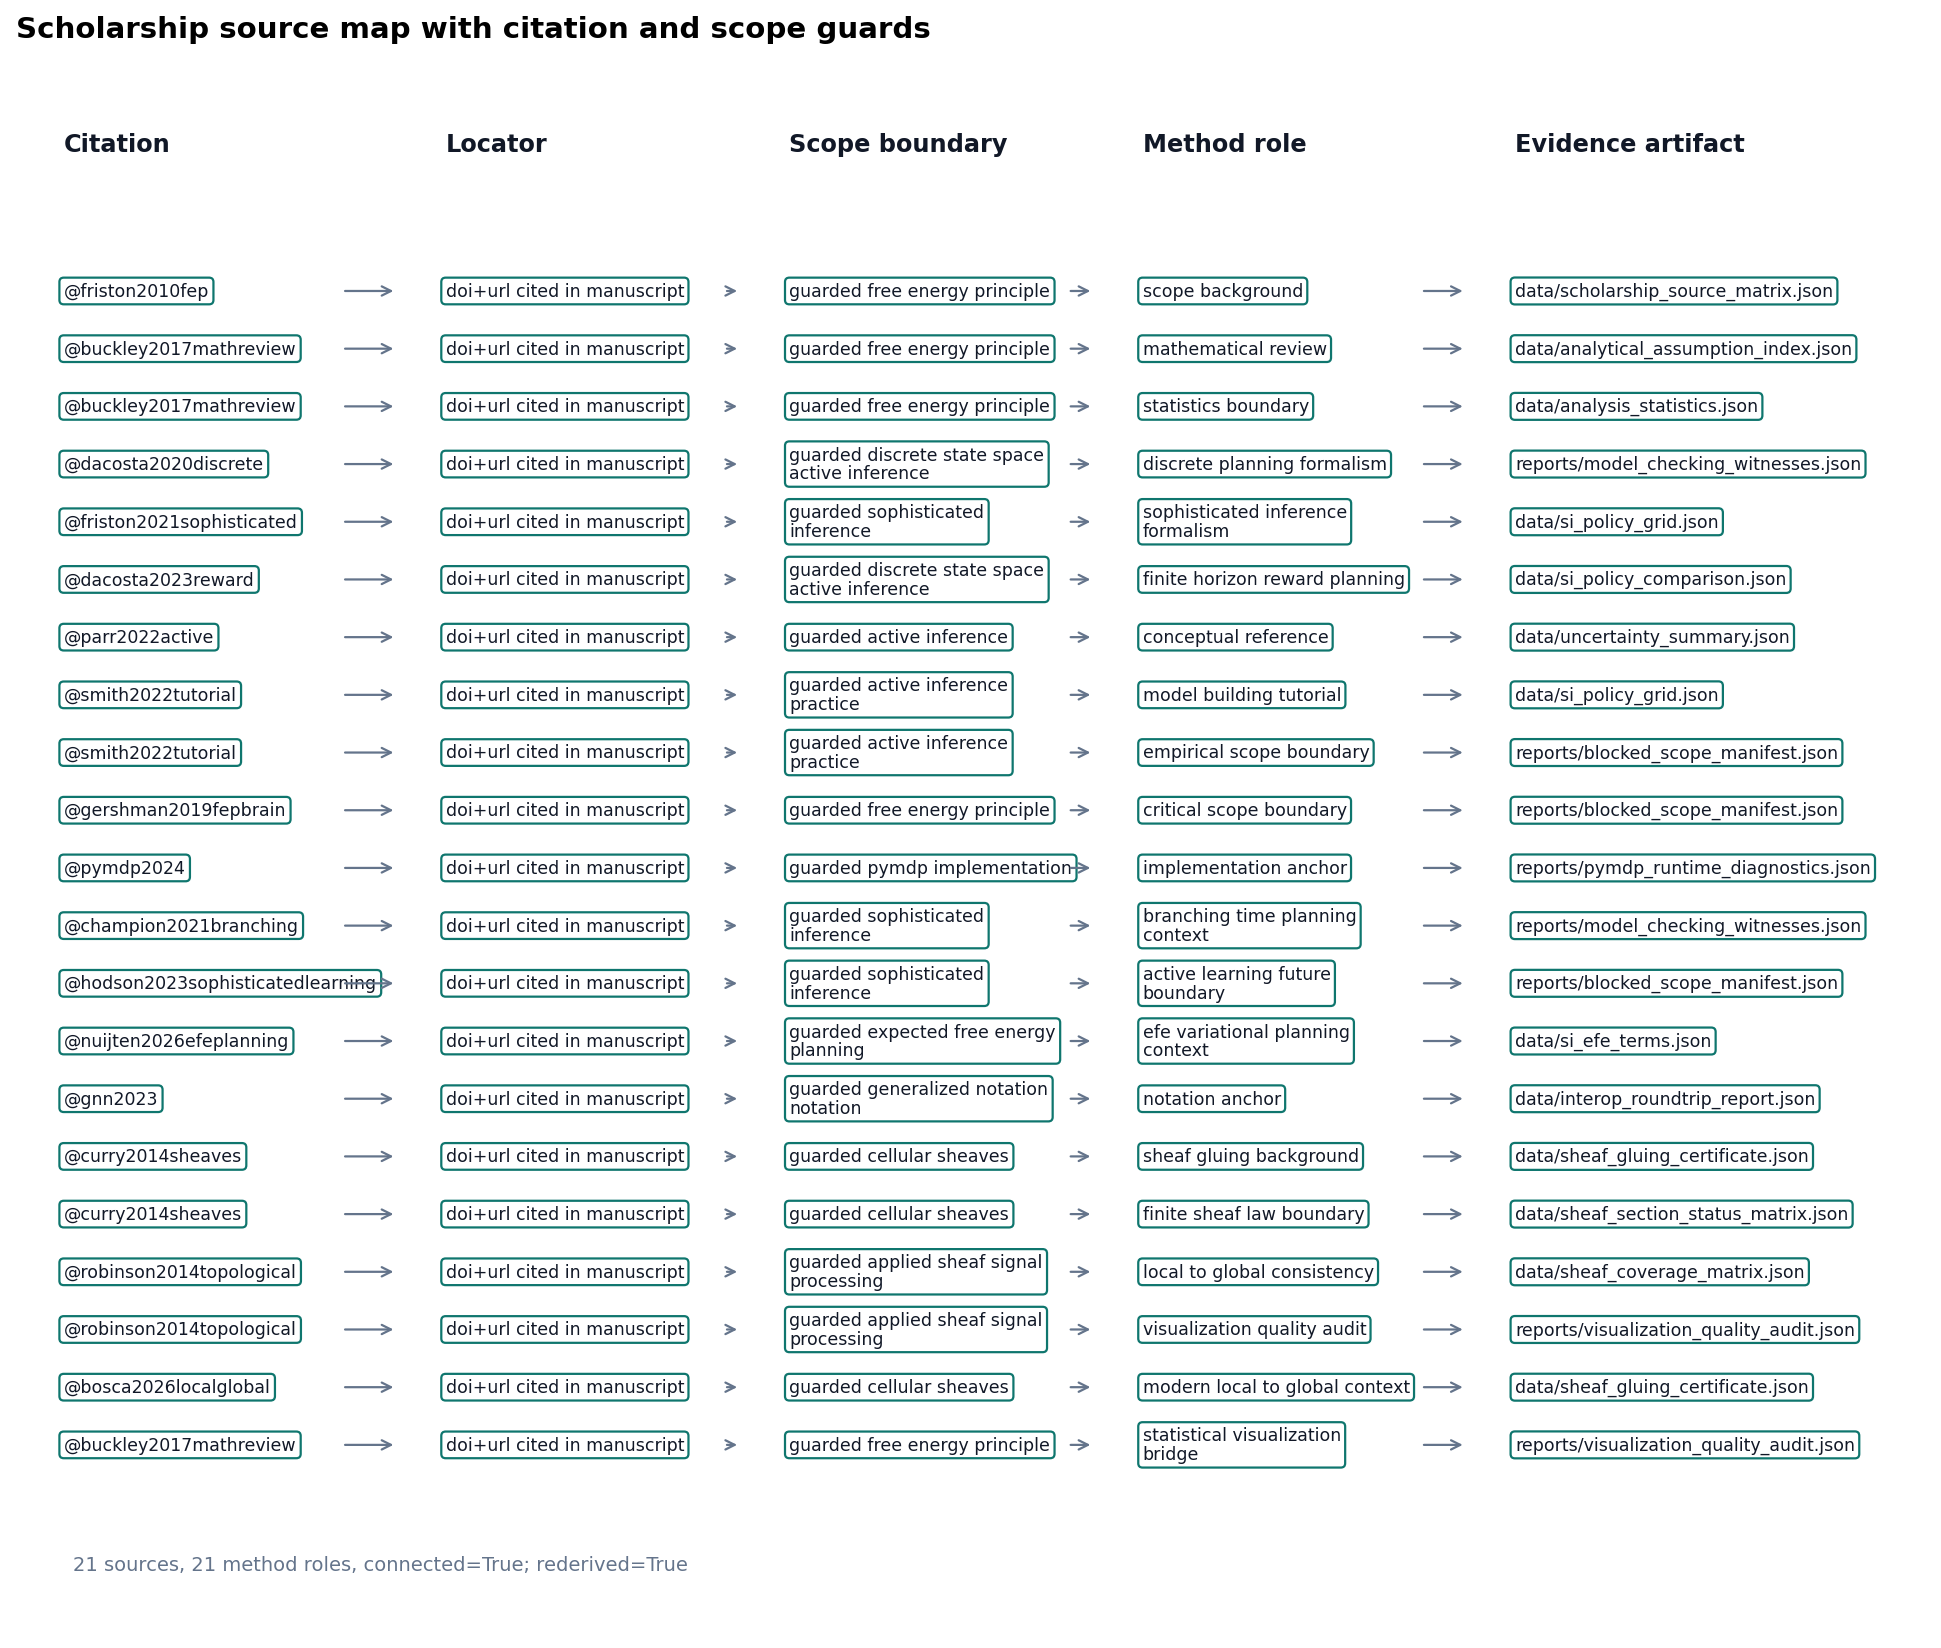
\includegraphics[width=0.95\linewidth,height=0.5\textheight,keepaspectratio]{../figures/scholarship_source_map.png}

\emph{Reproduced from fig.~\ref{fig:scholarship_source_map}. Scholarship
source map: 21 source rows across 21 method roles and 10 source
families. Connected status: true; row evidence rederived: true.}

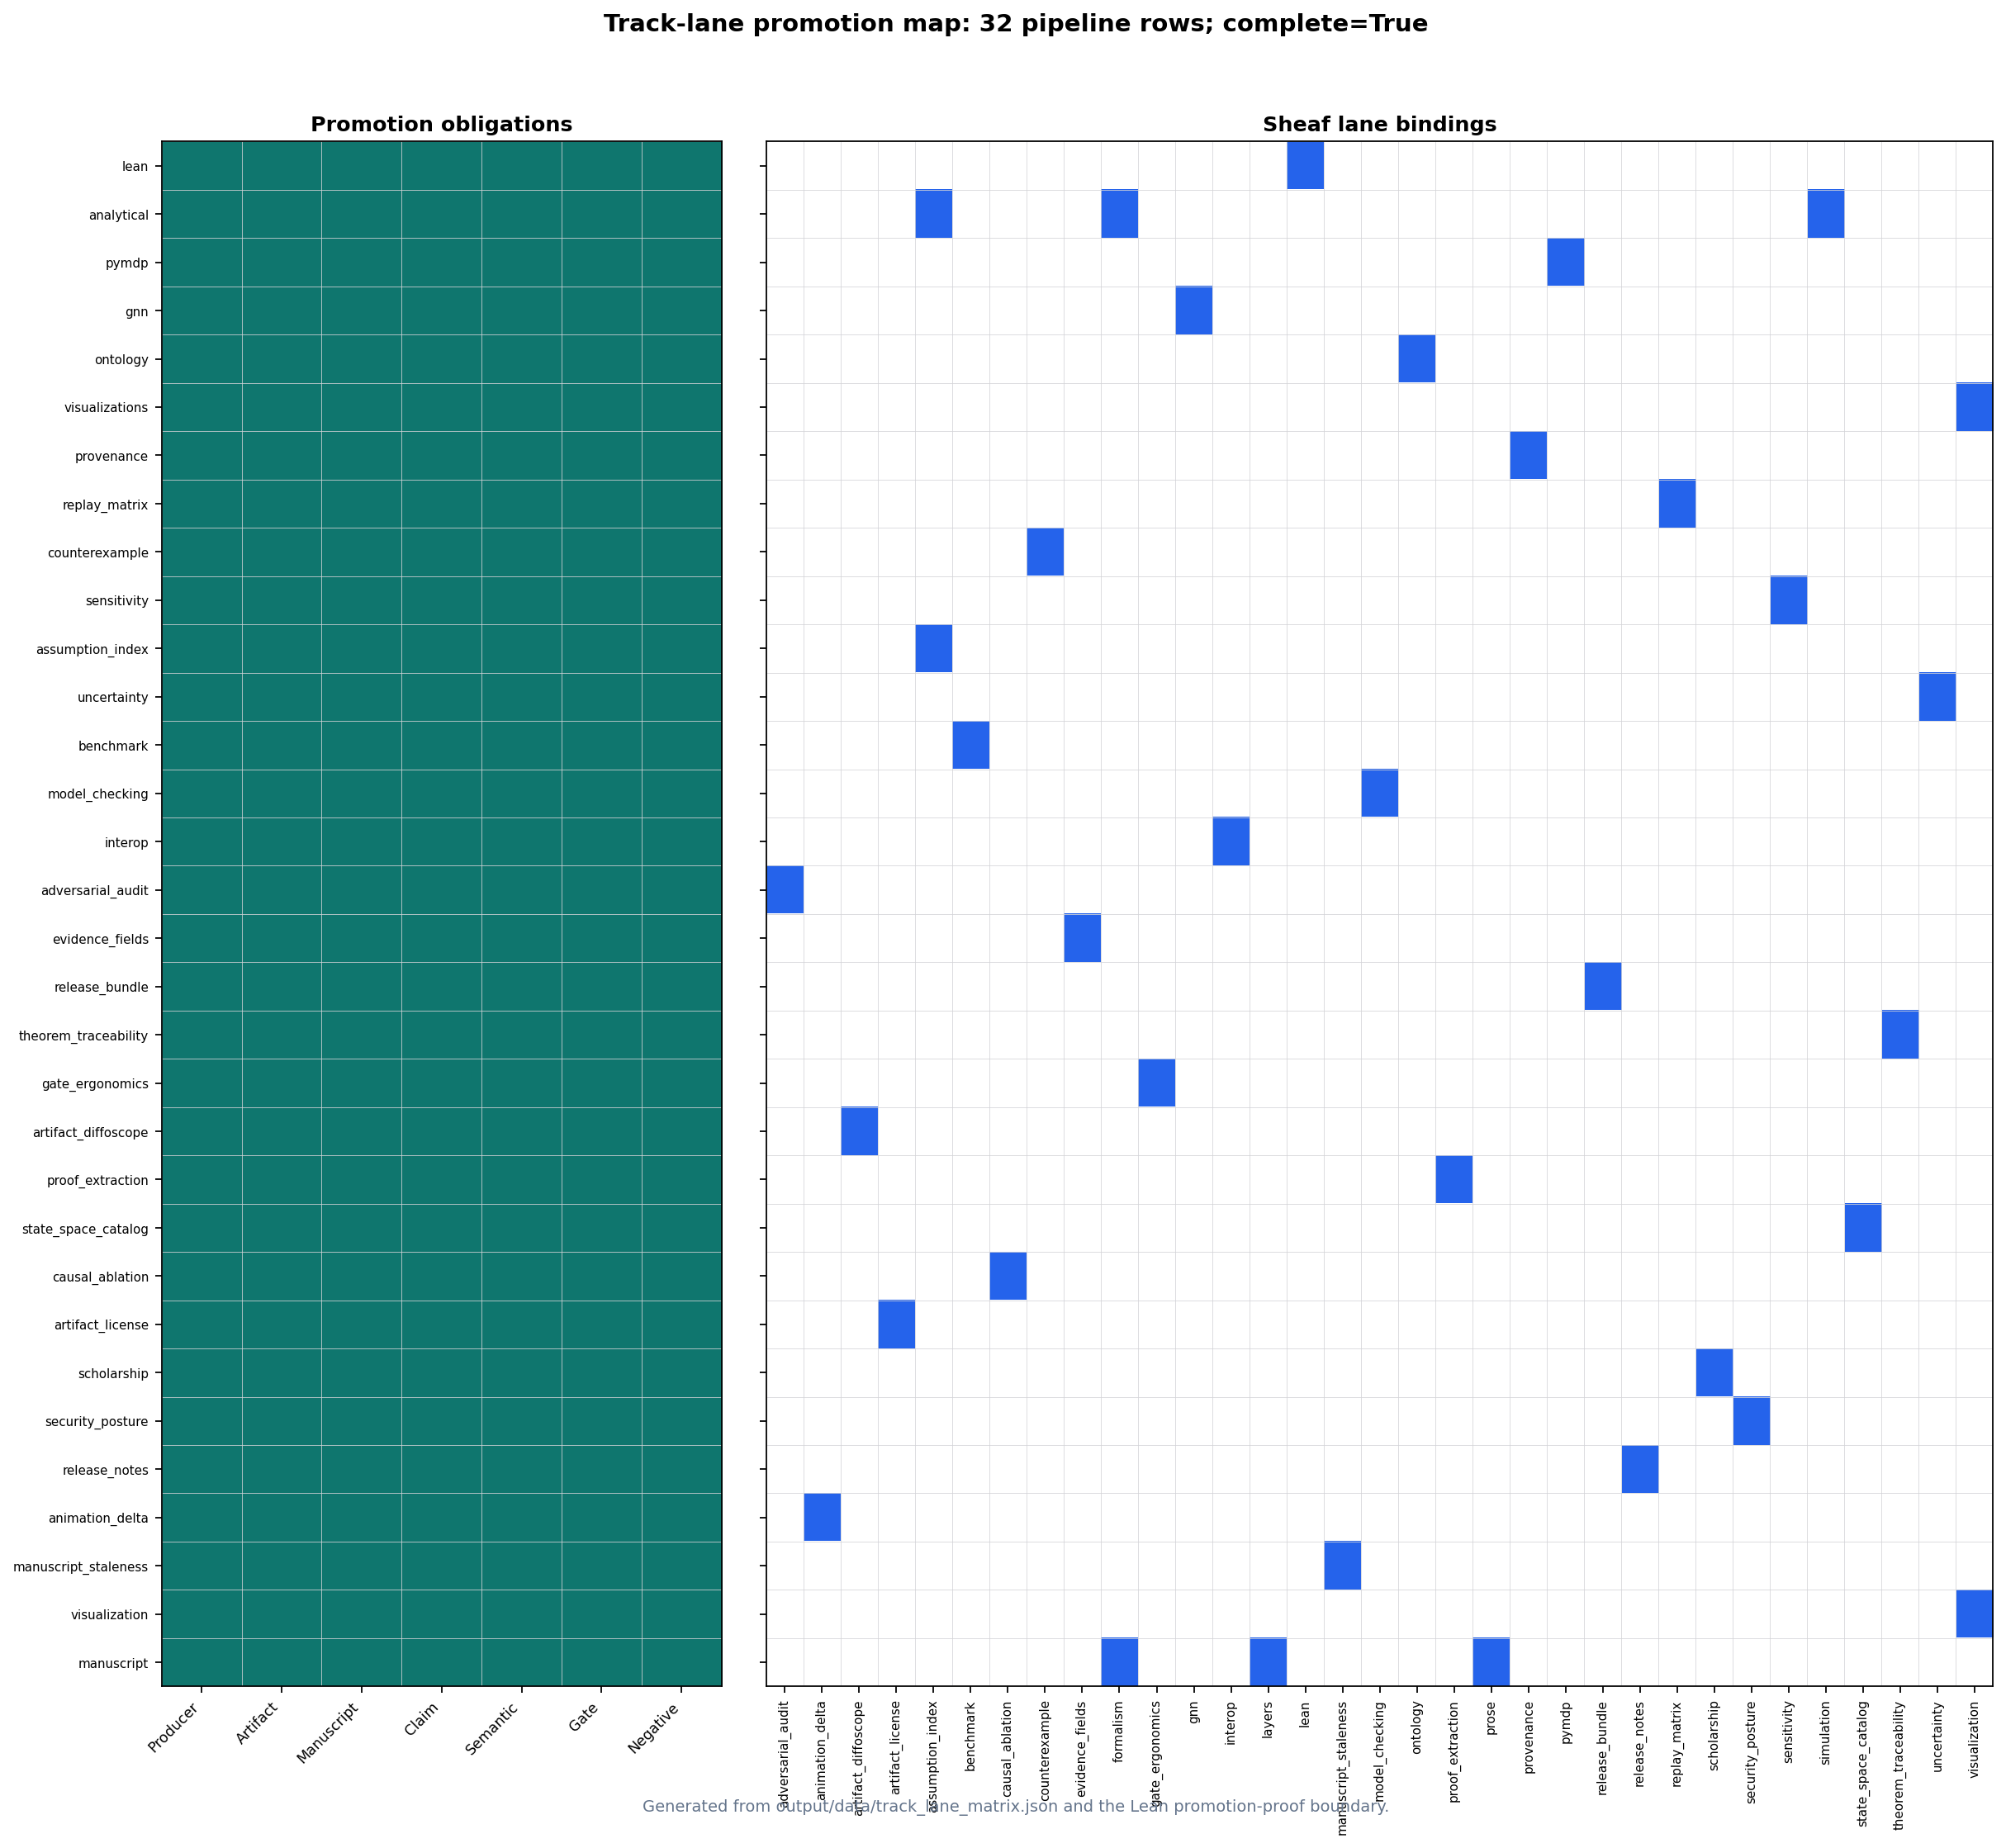
\includegraphics[width=0.98\linewidth,height=0.5\textheight,keepaspectratio]{../figures/track_lane_promotion_map.png}

\emph{Reproduced from fig.~\ref{fig:track_lane_promotion_map}.
Track-lane promotion map: 32 pipeline-to-sheaf rows with complete
promotion status true. Left: seven promotion-rule obligations; right:
sheaf fragment bindings.}

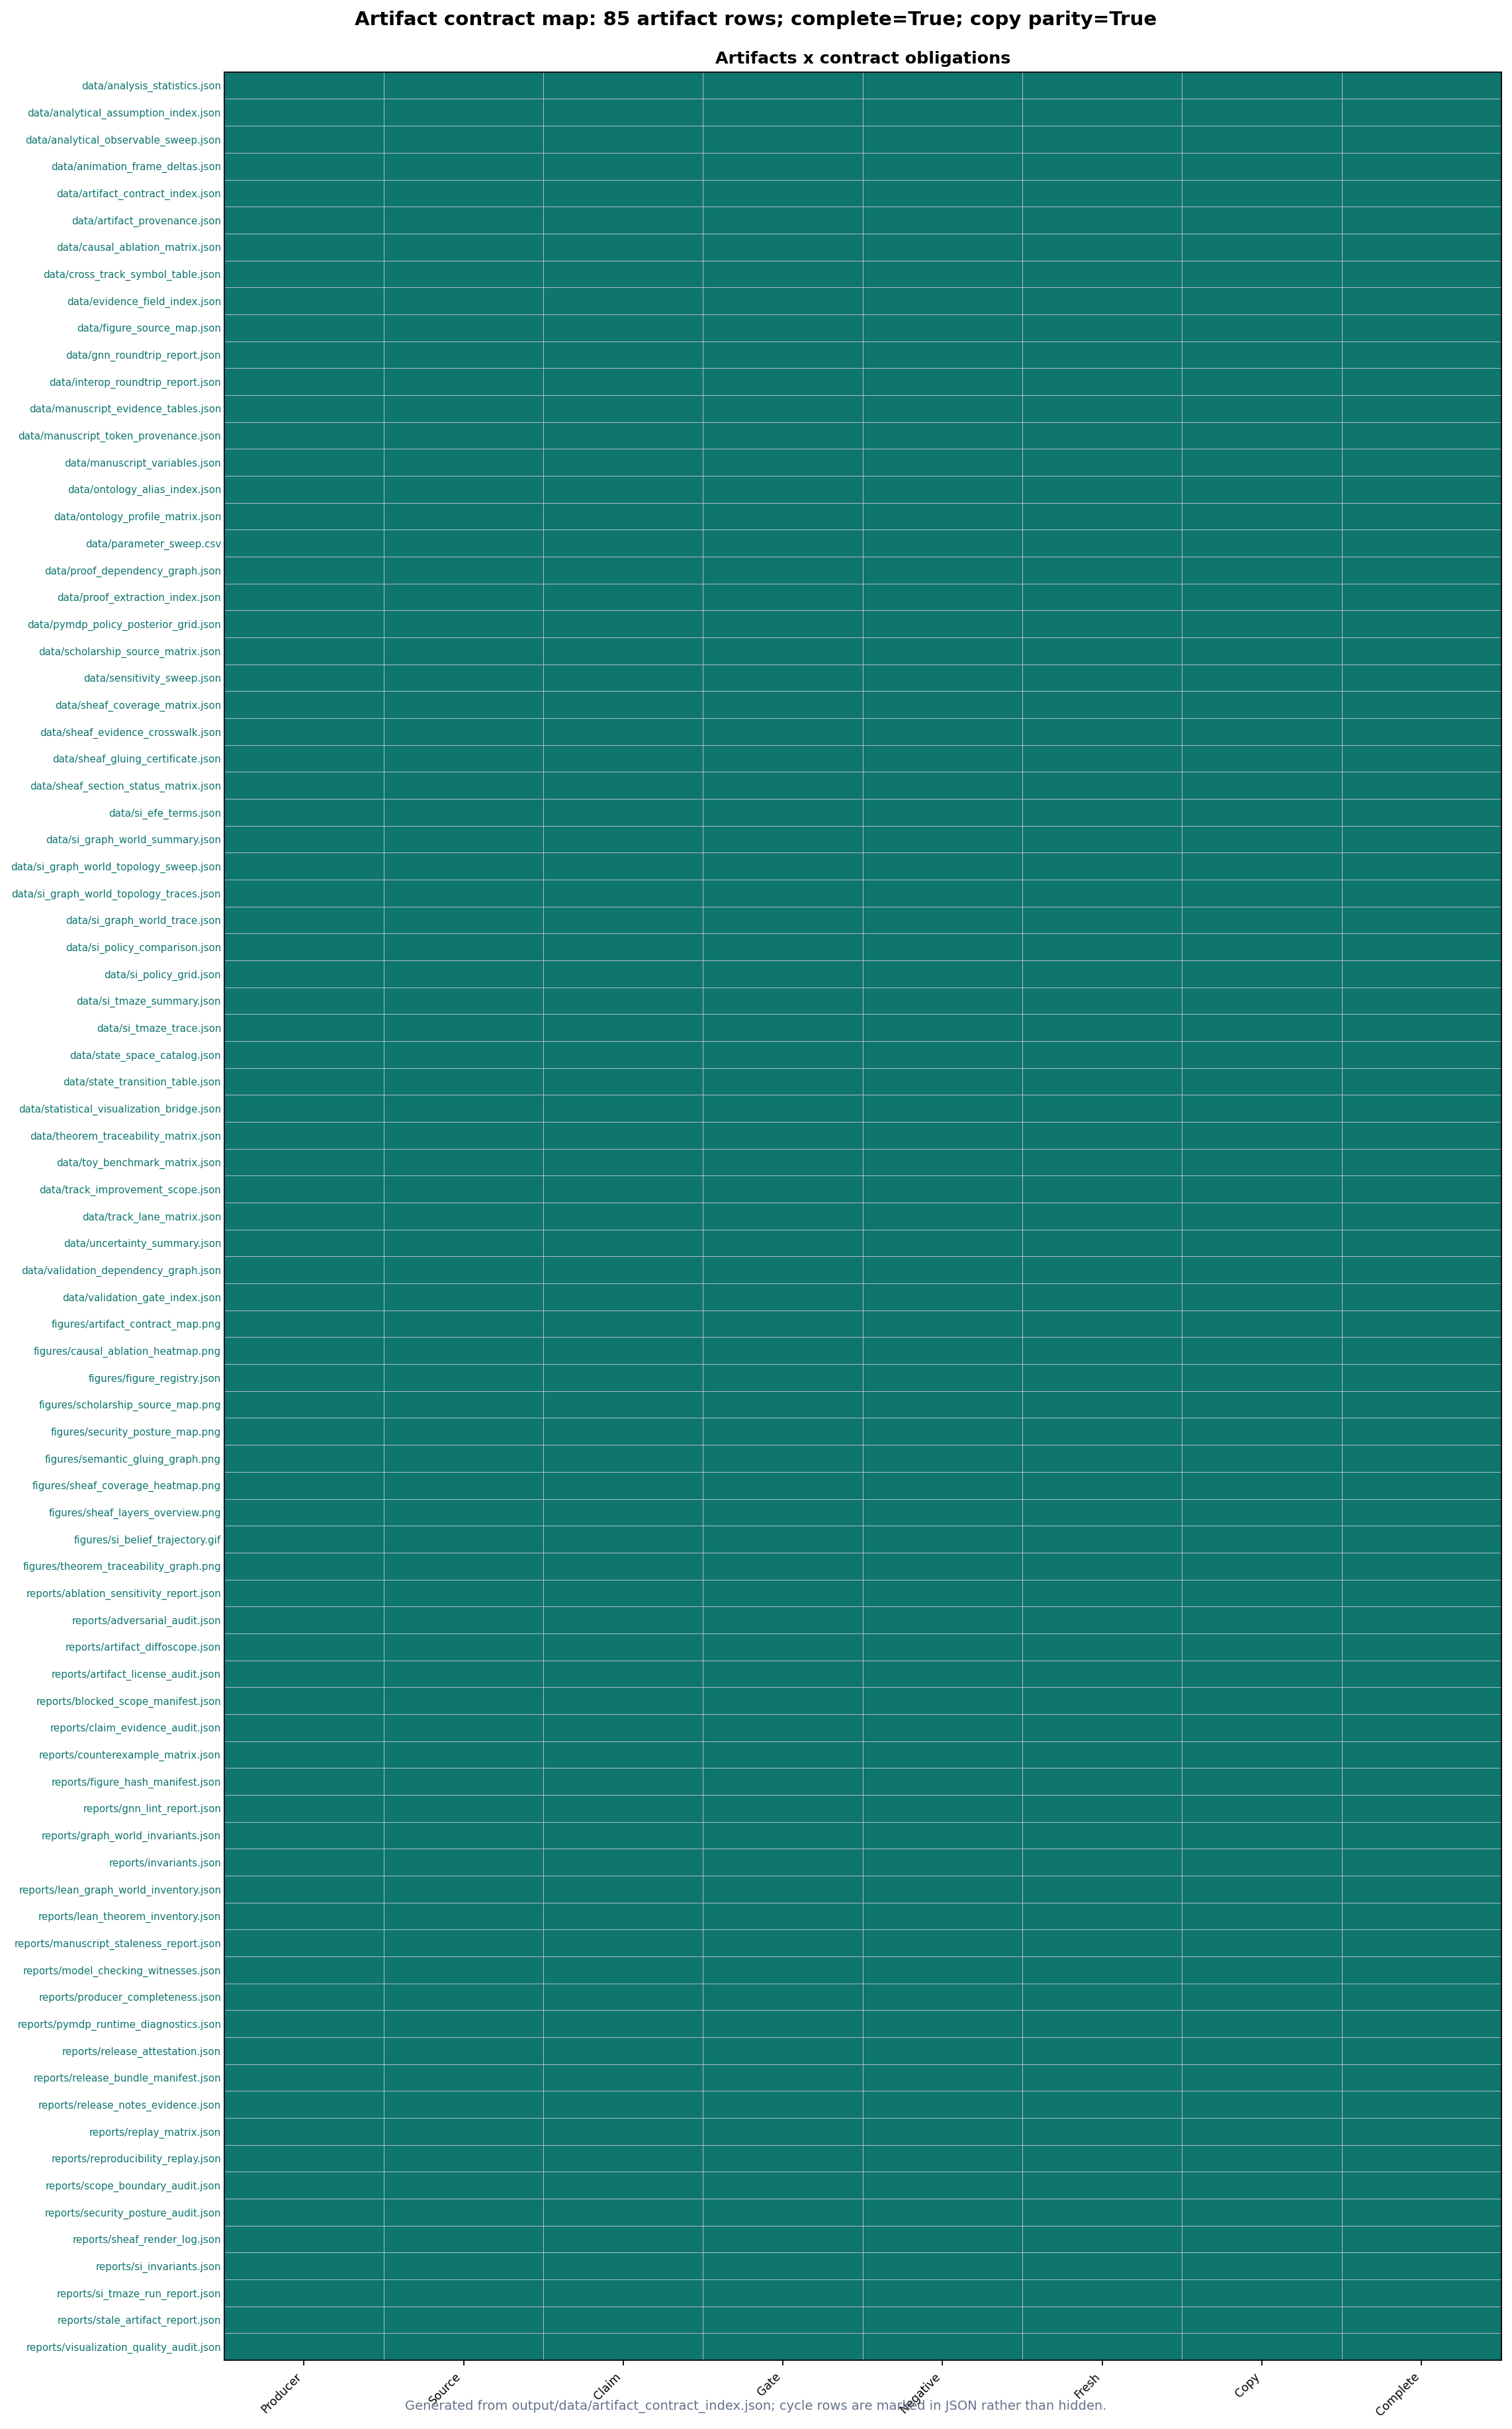
\includegraphics[width=0.98\linewidth,height=0.5\textheight,keepaspectratio]{../figures/artifact_contract_map.png}

\emph{Reproduced from fig.~\ref{fig:artifact_contract_map}. Artifact
contract map: 85 generated artifact rows with complete contract status
true and copied-output parity complete true. Cycle rows are explicit in
\breaktt{output/data/artifact\_contract\_index.json}.}

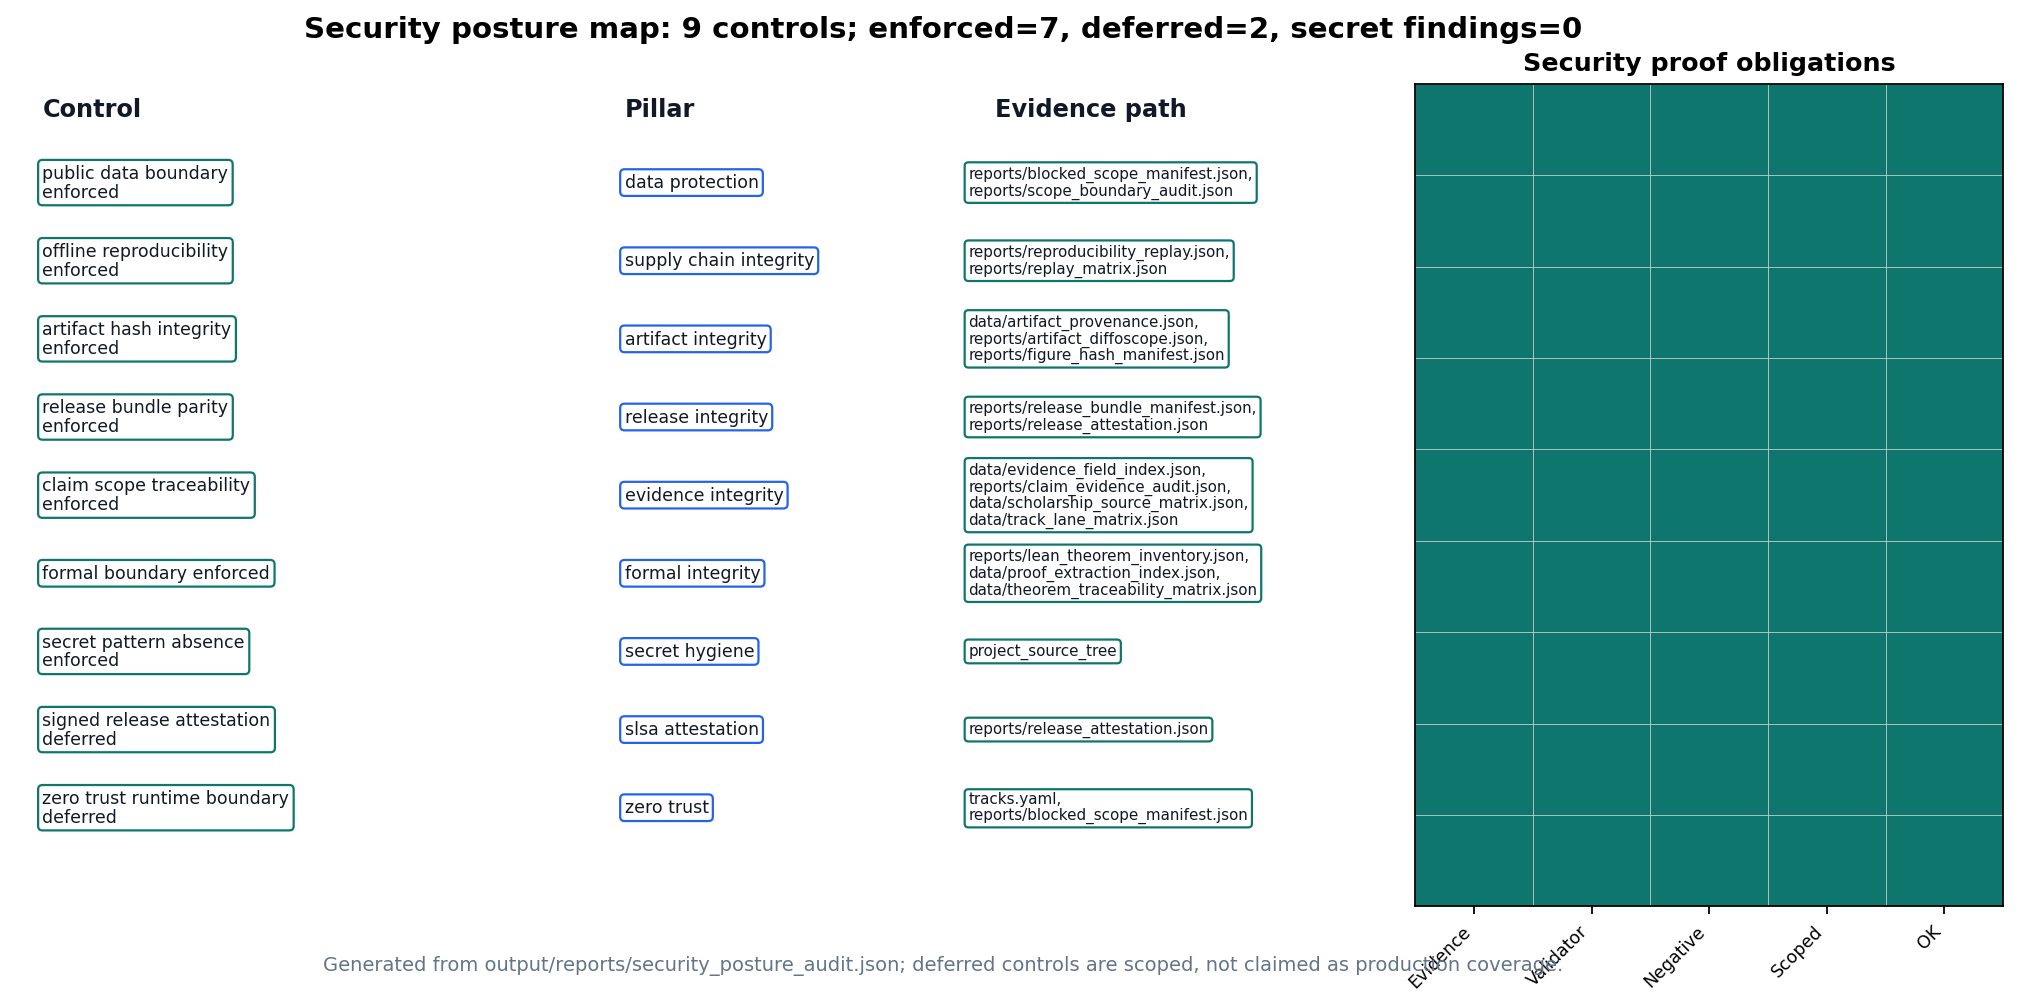
\includegraphics[width=0.96\linewidth,height=0.5\textheight,keepaspectratio]{../figures/security_posture_map.png}

\emph{Reproduced from fig.~\ref{fig:security_posture_map}. Security
posture map: 9 controls, 7 enforced and 2 scoped as deferred; secret
findings: 0; high-risk gaps: 0.}

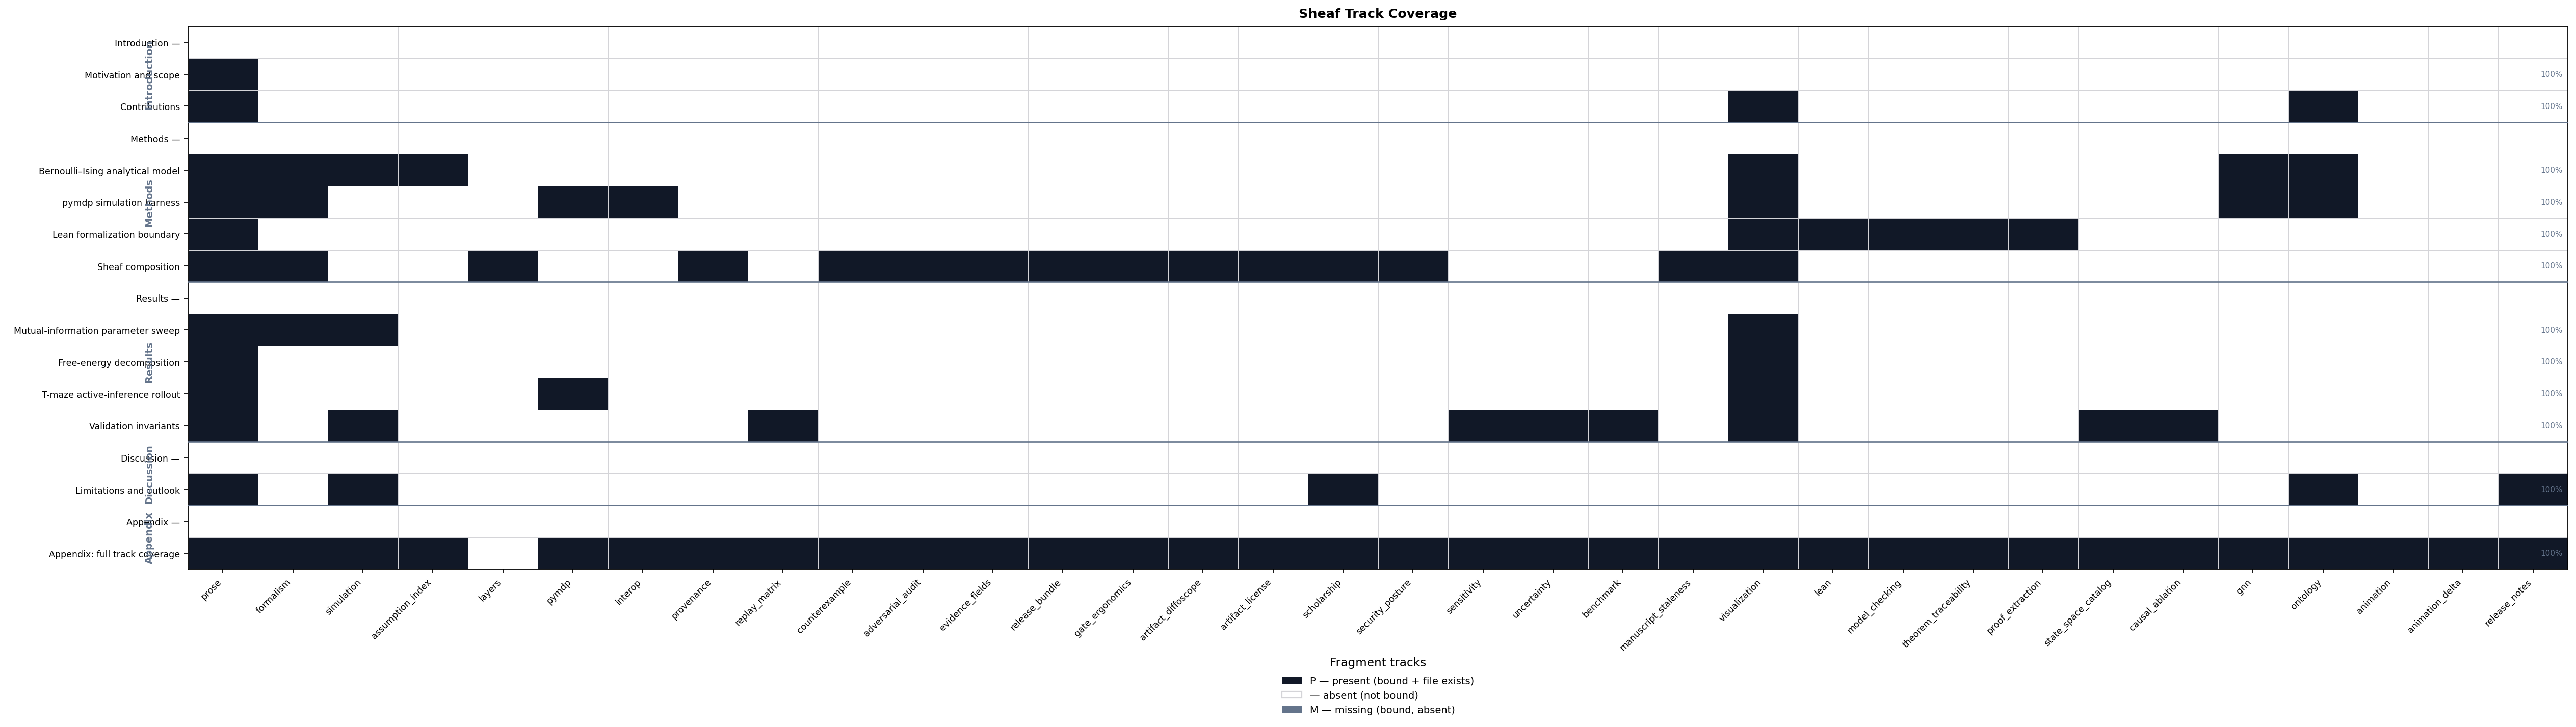
\includegraphics[width=0.95\linewidth,height=0.5\textheight,keepaspectratio]{../figures/sheaf_coverage_heatmap.png}

\emph{Reproduced from fig.~\ref{fig:sheaf_coverage_heatmap}. Sheaf track
coverage matrix: 17 IMRAD rows \texorpdfstring{\ensuremath{\times}}{x} 34 fragment columns. Black = present
(P), white = absent (---), gray = missing (M). Counts: 95 present / 95
bound / 0 missing. Generated from
\breaktt{output/data/sheaf\_coverage\_matrix.json}.}

Lean modules under \breaktt{lean/TemplateActiveInference/} declare
horizon and coupling witnesses. Build with \texttt{lake\ build} in
\texttt{lean/}; fig.~\ref{fig:lean_boundary_status} summarizes proved
versus deferred statements for this boundary fragment.

\breaktt{sheaf-track:model\_checking} binds
\breaktt{output/reports/model\_checking\_witnesses.json} and the Lean
theorem inventories. The appendix claim is exactly 12 finite exhaustive
witnesses with pass status \texttt{true}; Lean graph-world topology
coverage is 4 generated topology ids with all-witnessed flag
\texttt{true}.

\breaktt{theorem\_traceability\_matrix.json} provides the appendix proof
for theorem traceability: 17 linked rows with status \texttt{true}.

\subsubsection{Appendix track: proof
extraction}\label{appendix-track-proof-extraction}

\breaktt{proof\_extraction} binds
\breaktt{output/data/proof\_extraction\_index.json} into the full sheaf
appendix. Extracted theorems: 12. Constructive status: \texttt{true}.

The extraction index is intentionally modest: it records theorem names,
statements, source files, leading tactics, and forbidden proof-token
checks. That makes the Lean boundary inspectable without pretending that
every proof term has been translated into a proof object. A row with a
missing statement or forbidden token fails the formal interop gate and
the canonical sheaf gate.

\breaktt{output/data/proof\_dependency\_graph.json} adds the dependency
view used by the appendix figure. It contributes 207 theorem-source,
theorem-tactic, theorem-definition, and theorem-witness edges, with
resolved edge status \texttt{true}; this is the artifact that keeps the
theorem-traceability graph tied to generated Lean and model-checking
rows.

\subsubsection{Appendix track: state-space
catalog}\label{appendix-track-state-space-catalog}

\breaktt{state\_space\_catalog} binds
\breaktt{output/data/state\_space\_catalog.json} into the full sheaf
appendix. Rows: 6. All finite: \texttt{true}.

The catalog is the finite-scope boundary for every toy claim in the
exemplar. Each row records a model id, state count, action count, policy
count, source artifact, and finite flag; the validator recomputes that
counts are positive and that every row remains finite. This prevents a
manuscript sentence about exhaustive checking from silently drifting
into an unbounded or empirical setting.

\breaktt{output/data/state\_transition\_table.json} makes the boundary
operational. It contains 24 deterministic transition rows and covers all
reachable finite models with status \texttt{true}. Readers can therefore
audit not just the number of states, but the actual
state/action/next-state relation used by the model-checking witnesses.

\subsubsection{Appendix track: causal
ablation}\label{appendix-track-causal-ablation}

\texttt{causal\_ablation} binds
\breaktt{output/data/causal\_ablation\_matrix.json} into the full sheaf
appendix. Cells: 36. Complete grid: \texttt{true}.

The matrix is a finite teaching device: every row names a topology, a
coupling value, a perturbation, a scalar effect, and the generated
source row that made the effect admissible. It is not a claim about
empirical interventions. It shows how an intervention-shaped table can
be made falsifiable inside the sheaf: delete one perturbation cell or
clear one deterministic flag and the grid gate fails before the
manuscript can reuse the result.

\breaktt{output/reports/ablation\_sensitivity\_report.json} then joins
those ablation effects to the sensitivity and uncertainty artifacts. The
report contributes 36 source-backed rows, with source-backed status
\texttt{true}, so the appendix heatmap is a rendered view of validated
JSON rather than a decorative restatement.

GNN declarations: \breaktt{gnn/bernoulli\_toy.gnn.md} and
\breaktt{gnn/si\_tmaze.gnn.md} \citep{gnn2023}.
fig.~\ref{fig:gnn_ontology_concordance} and
sec.~\ref{sec:methods_analytical} document ontology concordance for the
Bernoulli toy; SI notation extends the same pattern under
sec.~\ref{sec:methods_pymdp}.

\subsubsection{Ontology bindings}\label{ontology-bindings-4}

\begin{itemize}
\tightlist
\item
  \texttt{belief\_entropy} \texorpdfstring{\ensuremath{\to}}{->} \textbf{BeliefEntropy}
\item
  \breaktt{expected\_free\_energy} \texorpdfstring{\ensuremath{\to}}{->} \textbf{ExpectedFreeEnergy}
\item
  \texttt{location} \texorpdfstring{\ensuremath{\to}}{->} \textbf{HiddenState}
\item
  \texttt{observation} \texorpdfstring{\ensuremath{\to}}{->} \textbf{ObservationLikelihood}
\item
  \texttt{policy} \texorpdfstring{\ensuremath{\to}}{->} \textbf{PolicyPosterior}
\item
  \texttt{sheaf\_track} \texorpdfstring{\ensuremath{\to}}{->} \textbf{SheafFragment}
\end{itemize}

Animation is an \textbf{extension} sheaf track backed by a deterministic
GIF from \breaktt{scripts/render\_animation.py}. This appendix row
documents the track binding only; default publication still uses static
SI figures (sec.~\ref{sec:results_si_tmaze},
fig.~\ref{fig:si_tmaze_actions}) while the GIF remains an auditable
generated artifact.

The appendix \texttt{animation\_delta} row points to
\breaktt{output/data/animation\_frame\_deltas.json}. The manifest records
3 adjacent-frame deltas, with \texttt{true} as the hydrated evidence
that the GIF is trace-derived rather than a duplicated static frame.

\subsubsection{Appendix track: release notes
evidence}\label{appendix-track-release-notes-evidence}

\texttt{release\_notes} binds
\breaktt{output/reports/release\_notes\_evidence.json} into the full
sheaf appendix. Rows: 3. Source-backed: \texttt{true}.

Release notes are treated as claims, not as informal changelog prose.
Each row names a source artifact and a pass/deferred status, so the
release note can say only what validation, bundle, or semantic artifacts
support. The validator re-derives support from rows; flipping the
summary bit without fixing a failed row still fails.

\breaktt{output/reports/release\_attestation.json} is the compact final
view over the same boundary. It records 7 attestation rows for
validation, release bundle hash, license audit, semantic certificate,
and blocked-scope status, with all-attested flag \texttt{true}.

\newpage

\section{Conclusion}\label{sec:conclusion}

Analytical oracles (sec.~\ref{sec:methods_analytical}), pymdp rollouts
(sec.~\ref{sec:results_si_tmaze}), and sheaf composition
(sec.~\ref{sec:methods_sheaf}) share one auditable manuscript contract:
measured artifacts hydrate 12 composed sections,
sec.~\ref{sec:sheaf_coverage} reports binding state, and strict compose
validation blocks gray matrix cells before PDF rendering.

The T-maze harness runs in \texttt{state\_inference} mode with config
hash \breaktt{81eb061f43b7bfd7}; sweep RMSE 0 nats summarizes
analytical-empirical agreement on the toy coupling grid.
sec.~\ref{sec:results_invariants} merges analytical and simulation
gates; sec.~\ref{sec:discussion_outlook} states scope and extensions.
Scientific claims remain confined to declared models, not empirical
statements about biological agents \citep{gershman2019fepbrain}.

The exemplar therefore sits at a narrow intersection: finite discrete
active inference on POMDP-like toy models
\citep{dacosta2020discrete, friston2021sophisticated, dacosta2023reward},
sheaf-style local-to-global checks for publication artifacts
\citep{curry2014sheaves, robinson2014topological}, and GNN notation as
an interop layer \citep{gnn2023}.

\newpage

\section{References}\label{references}

See \breaktt{manuscript/references.bib} for bibliography entries cited in
the composed sections.

\newpage



\clearpage

\bibliography{references}
% transmission-end-bookend
\clearpage
\thispagestyle{empty}
\setlength{\parskip}{0pt}
\setlength{\itemsep}{0pt}
\begin{samepage}
\scriptsize

\section*{END OF TRANSMISSION}\label{end-of-transmission}

\textbf{Release:} v0.3.2 \texorpdfstring{\ensuremath{\cdot}}{.} DOI \breaktt{10.5281/zenodo.20417021} \texorpdfstring{\ensuremath{\cdot}}{.}
SHA-256 \texttt{f191b48f9439…} \texorpdfstring{\ensuremath{\cdot}}{.} pairing complete

\begin{figure}
\centering
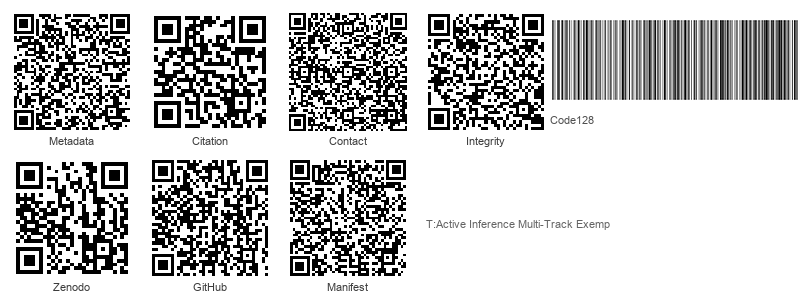
\includegraphics[width=0.88\linewidth,height=0.5\textheight,keepaspectratio,alt={Integrity QR strip}]{../figures/transmission_integrity_strip.png}
\caption{Integrity QR strip}
\end{figure}

\textbf{Prior:} \emph{No prior releases.}

\end{samepage}

\end{document}
